\documentclass[letterpaper,10pt]{book}
% Change to 10 pt
\usepackage{pdfpages}
\usepackage{morewrites}			% to counteract the no write space problem
\setcounter{tocdepth}{6}

\usepackage[framemethod=TikZ]{mdframed}

\usepackage{fancyhdr}

\usepackage{paralist}
\usepackage{amsmath}
\usepackage{amsfonts}
\usepackage{amssymb}
\usepackage{graphicx}

\usepackage{datetime}
%\usepackage{ulem}

%\usepackage[nottoc]{toobibind}

\usepackage[inline]{enumitem}

% Outer margin at 2.50 is exacty correct to fit the ``corruption alert'' tables
\usepackage[inner=1.0in, outer=2.50in, top=2.54cm,bottom=2.54cm, marginparwidth=2.25in]{geometry}

\usepackage{marginnote}
\usepackage{longtable}
\usepackage{booktabs}
\usepackage{xcolor}

\usepackage{soul}

%%%%%%%%%%%%
\definecolor{ForestGreen}{rgb}{0.00,0.29,0.098}
%%%%%%%%%%%%

\usepackage{marginnote}

\usepackage{imakeidx} 
\usepackage[
	backref=true,
	style=numeric,
%	citestyle=numeric,
	backend=bibtex
	]{biblatex}
\usepackage[driverfallback=hypertex,colorlinks=True]{hyperref}
\usepackage{cleveref}

\makeindex[name=scripture,columnsep=20pt, columnseprule=True,columns=3, title=Scripture References]
\makeindex[name=speaker,columnsep=20pt, columnseprule=True,,columns=2, title=Sermon Creator]
\makeindex[name=series,columnsep=20pt, columnseprule=True,,columns=2, title=Sermon Series]
\makeindex[name=date,columnsep=20pt, columnseprule=True,columns=2, title=Sermon Date]
\makeindex[name=event,columnsep=20pt, columnseprule=True,columns=2, title=Event]
\makeindex[name=topic,columnsep=20pt, columnseprule=True,columns=2, title=Topic]
\makeindex[name=AWIP,columnsep=20pt, columnseprule=True,columns=3, title=All Words in Passage]
\makeindex[name=NWIV,columnsep=20pt, columnseprule=True,columns=3, title=Number of Words in Verse]
\makeindex[name=PNIP,columnsep=20pt, columnseprule=True,columns=3, title=Proper Names in Passage]
\makeindex[name=PEIP,columnsep=20pt, columnseprule=True,columns=2, title=Prophetic Events in Passage]
\makeindex[name=TWPAQ,columnsep=20pt, columnseprule=True,columns=1, title=13-Word Phrases and Quotes]
\makeindex[name=PFTTIS,columnsep=20pt, columnseprule=False,columns=3, title=Phrases found 13 times in scripture]
\makeindex[name=WFTTIS,columnsep=20pt, columnseprule=False,columns=3, title=Words found 13 times in scripture]
\makeindex[name=WFITV,columnsep=20pt, columnseprule=False,columns=3, title=Words found in exactly 13 verses]
\makeindex[name=EVENTS,columnsep=20pt, columnseprule=False,columns=2, title=Sermon Log by Place]
\makeindex[name=QUESTIONS,columnsep=20pt, columnseprule=False,columns=2, title=Bible Questions]
\makeindex[name=DOCTRINES,columnsep=20pt, columnseprule=False,columns=2, title=Doctrines]
\makeindex[name=SONGS,columnsep=20pt, columnseprule=False,columns=1, title=Songs]
\makeindex[name=LOCATION,columnsep=20pt, columnseprule=False,columns= 2, title=Location]
\makeindex[name=FACEBOOK,columnsep=20pt, columnseprule=False,columns=2, title=Facebook]
\makeindex[name=DEVOTIONAL,columnsep=20pt, columnseprule=False,columns=2, title=Devotional Items]
%%%%%%%%%%%%%%%%% EXTRA COLORS
\definecolor{champagne}{rgb}{0.97,0.91,0.81}
\definecolor{bone}{rgb}{0.89,0.85,0.79}
\pagestyle{fancy}
\fancyhf{}
\fancyhead[LE,RO]{\today}
\fancyhead[RE,LO]{Daily Bible Reading}
\fancyhead[CE,CO]{-page \thepage  - }

\fancyfoot[CO,CE]{\leftmark}
%\fancyfoot[LE,RO]{CSCE 692, HW1}

\title{DBR\\
Daily \\ Reads}
\author{Keith Anthony \\
\today }
%+/ffffff +   \pagenumbering{gobble}
\bibliography{Bibliographies/All20220122}

\setlength{\fboxsep}{1.0pt}

\usepackage[utf8]{inputenc}
\usepackage{tikz}

\begin{document}
%%%%%%%%%%%% Tile Page

\begin{titlepage}

\begin{flushright}
\rightskip=-2.5cm
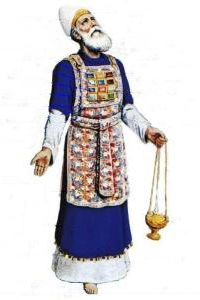
\includegraphics[width=50mm,scale=1.5]{Extras/Melchisedec.jpg}
\vspace{0.4in}  % Create a title for the document and write it in bold font
\LARGE{\textbf{\date}} % Again, do a line break
\linebreak 
% Create a subtitle \large{with Outlines, Statistics, Cross References, and Notes}
\vspace{0.5in}
\begin{flushleft}
\LARGE{Day \#79: Sunday, 20  March 2022 LITE  \\}\vspace{0.25in}
\LARGE{Judges 19-21 Psalm 79 Proverb 20}
\end{flushleft}
\vspace{0.6in}
\bigskip

\normalsize{Xenia, Oh.\\}
\normalsize{created: \today}
\vspace{1.3in}

\end{flushright}
\end{titlepage}

\newpage 
\tableofcontents\hypertarget{TOC}{}
\listoffigures
\listoftables

\hyphenation{A-bim-e-lech bre-thren E-phra-im  Gib-e-o-nites Jer-u-sa-lem through-out Phil-i-stines The-o-phil-us Am-a-le-kites ven-geance Mesh-el-e-mi-ah onan-ism Phar-a-oh thoughts grev-ous-ness Hach-a-liah adul-ter-er Shad-rach}

%%%%%%%%%%%%%%%%% EXTRA COLORS
%%%%%%%%%%%%%%%%% EXTRA COLORS
%%%%%%%%%%%%%%%%% EXTRA COLORS
\definecolor{champagne}{rgb}{0.97,0.91,0.81}
\definecolor{bone}{rgb}{0.89,0.85,0.79}

\definecolor{ForestGreen}{rgb}{0.00,0.29,0.098}
\definecolor{GIVING}{cmyk}{1,0.0,0.72,.1}

\definecolor{MLPE}{cmyk}{1,1,0,.45}
\definecolor{SOCCER}{cmyk}{.77, 0, .42, .49}
\definecolor{PAYBILL}{cmyk}{0,0.83,0.76,0.07}
\definecolor{SERMON}{cmyk}{.14,.9,0,.30} % aka seance \href{http://www.flatuicolorpicker.com/purple-cmyk-color-model/}{seance}
\definecolor{BIBLE}{cmyk}{0,.17,.74,.17}
\definecolor{WORKBLUE}{cmyk}{1, .5, 0, .6}
\definecolor{myOrange}{cmyk}{0, .4, .98, .03}
\definecolor{myTan}{cmyk}{0.0,.07,.17,.10}
\definecolor{myRed}{cmyk}{0,1,1,0}
\definecolor{myWhite}{cmyk}{0,0,0,0}
\definecolor{BLUESoD}{cmyk}{.97,.84,0,.04}
\definecolor{WHITE}{cmyk}{0,0,0,0}
\definecolor{OLDGOLD}{cmyk}{0.05,0.3,1.00,0}
\definecolor{CASTLETON}{cmyk}{1,0,0.31,0.66}
\definecolor{cadmiumgreen}{rgb}{0.0, 0.42, 0.24}
\definecolor{jungle}{rgb}{0.203,0.4882,0.1718}
\definecolor{MYGOLD}{rgb}{1,.84,0}

\definecolor{MYLIGHTGRAY}{rgb}{.85,.85,.85}

\definecolor{codegreen}{rgb}{0,0.6,0}
\definecolor{codegray}{rgb}{0.5,0.5,0.5}
\definecolor{codepurple}{rgb}{0.58,0,0.82}
\definecolor{backcolour}{rgb}{0.95,0.95,0.92}


\mdfdefinestyle{MyFrame}{%
    linecolor=blue,
    outerlinewidth=2pt,
    roundcorner=5pt,
    innertopmargin=\baselineskip,
    innerbottommargin=\baselineskip,
    innerrightmargin=10pt,
    innerleftmargin=10pt,
    backgroundcolor=gray!25!white}


\mdfdefinestyle{MyFrame2}{%
    linecolor=black,
    outerlinewidth=2pt,
    roundcorner=5pt,
    innertopmargin=\baselineskip,
    innerbottommargin=\baselineskip,
    innerrightmargin=10pt,
    innerleftmargin=10pt,
    backgroundcolor=yellow!25!white}


%%%%%
%% for PFTTIS list
%%%%%

%%% And Joseph said unto
\index[PFTTIS]{And Joseph said unto!Genesis!Gen 40:008}
\index[PFTTIS]{And Joseph said unto!Genesis!Gen 40:012}
\index[PFTTIS]{And Joseph said unto!Genesis!Gen 41:025}
\index[PFTTIS]{And Joseph said unto!Genesis!Gen 42:014}
\index[PFTTIS]{And Joseph said unto!Genesis!Gen 42:018}
\index[PFTTIS]{And Joseph said unto!Genesis!Gen 44:015}
\index[PFTTIS]{And Joseph said unto!Genesis!Gen 45:003}
\index[PFTTIS]{And Joseph said unto!Genesis!Gen 45:004}
\index[PFTTIS]{And Joseph said unto!Genesis!Gen 46:031}
\index[PFTTIS]{And Joseph said unto!Genesis!Gen 48:009}
\index[PFTTIS]{And Joseph said unto!Genesis!Gen 48:018}
\index[PFTTIS]{And Joseph said unto!Genesis!Gen 50:019}
\index[PFTTIS]{And Joseph said unto!Genesis!Gen 50:024}


%%% a shadow
\index[PFTTIS]{a shadow!1Chronicles!1Chr 029:15}
\index[PFTTIS]{a shadow!Job!Job 008:09}
\index[PFTTIS]{a shadow!Job!Job 014:02}
\index[PFTTIS]{a shadow!Job!Job 017:07}
\index[PFTTIS]{a shadow!Psalm!Psa 102:011}
\index[PFTTIS]{a shadow!Psalm!Psa 144:004}
\index[PFTTIS]{a shadow!Ecclesiastes!Eccl 006:012}
\index[PFTTIS]{a shadow!Ecclesiastes!Eccl 008:013}
\index[PFTTIS]{a shadow!Isaiah!Isa 04:006}
\index[PFTTIS]{a shadow!Isaiah!Isa 25:004}
\index[PFTTIS]{a shadow!Jonah!Jnh 04:06}
\index[PFTTIS]{a shadow!Colossians!Col 02:017}
\index[PFTTIS]{a shadow!Hebews!Heb 10:001}

%%% blessed is the man
\index[PFTTIS]{blessed is the man!Psalm!Psa 001:001}
\index[PFTTIS]{blessed is the man!Psalm!Psa 032:002}
\index[PFTTIS]{blessed is the man!Psalm!Psa 034:008}
\index[PFTTIS]{blessed is the man!Psalm!Psa 065:004}
\index[PFTTIS]{blessed is the man!Psalm!Psa 084:005}
\index[PFTTIS]{blessed is the man!Psalm!Psa 084:012}
\index[PFTTIS]{blessed is the man!Psalm!Psa 094:012}
\index[PFTTIS]{blessed is the man!Psalm!Psa 112:001}
\index[PFTTIS]{blessed is the man!Proverbs!Pro 008:034}
\index[PFTTIS]{blessed is the man!Isaiah!Isa 056:002}
\index[PFTTIS]{blessed is the man!Jeremiah!Jer 017:007}
\index[PFTTIS]{blessed is the man!Romans!Rom 004:008}
\index[PFTTIS]{blessed is the man!James!Jam 001:012}


%%% carry them
\index[PFTTIS]{carry them!Leviticus!Lev 14:045}
\index[PFTTIS]{carry them!Numbers!Num 11:012}
\index[PFTTIS]{carry them!Joshua!Jsh 04:003}
\index[PFTTIS]{carry them!1Samuel!1Sam 20:040}
\index[PFTTIS]{carry them!1Kings!1Kng 08:046}
\index[PFTTIS]{carry them!2Chronicles!2Chr 06:036}
\index[PFTTIS]{carry them!Ezra!Ezra 05:015}
\index[PFTTIS]{carry them!Isaiah!Isa 40:011}
\index[PFTTIS]{carry them!Isaiah!Isa 41:016}
\index[PFTTIS]{carry them!Isaiah!Isa 57:013}
\index[PFTTIS]{carry them!Jeremiah!Jer 20:004}
\index[PFTTIS]{carry them!Jeremiah!Jer 20:005}
\index[PFTTIS]{carry them!Jeremiah!Jer 43:012}


\index[PFTTIS]{good tidings!2Samuel!2Sam 18:027}
\index[PFTTIS]{good tidings!1Kings!1Ki 01:042}
\index[PFTTIS]{good tidings!2Kings!2Ki 07:009 (2x)}
\index[PFTTIS]{good tidings!Isaiah!Isa 40:009 (2x)}
\index[PFTTIS]{good tidings!Isaiah!Isa 41:007}
\index[PFTTIS]{good tidings!Isaiah!Isa 52:007}
\index[PFTTIS]{good tidings!Isaiah!Isa 61:001}
\index[PFTTIS]{good tidings!Nahum!Nah 01:005}
\index[PFTTIS]{good tidings!Luke!Lk 02:010}
\index[PFTTIS]{good tidings!1Thessalonians!1Thess 03:006}


%%% dead body
\index[PFTTIS]{dead body!Leviticus!Lev 21:011}
\index[PFTTIS]{dead body!Numbers!Num 06:006}
\index[PFTTIS]{dead body!Numbers!Num 09:006}
\index[PFTTIS]{dead body!Numbers!Num 09:007}
\index[PFTTIS]{dead body!Numbers!Num 09:010}
\index[PFTTIS]{dead body!Numbers!Num 09:011}
\index[PFTTIS]{dead body!Numbers!Num 09:013}
\index[PFTTIS]{dead body!Numbers!Num 09:016}
\index[PFTTIS]{dead body!2Kings!2Ki 08:005}
\index[PFTTIS]{dead body!Isaiah!Isa 26:019}
\index[PFTTIS]{dead body!Jeremiah!Jer 26:023}
\index[PFTTIS]{dead body!Jeremiah!Jer 36:030}
\index[PFTTIS]{dead body!Haggai!Hag 02:013}

%%% great sea
\index[PFTTIS]{great sea!Numbers!Num 34:006}
\index[PFTTIS]{great sea!Numbers!Num 34:007}
\index[PFTTIS]{great sea!Joshua!Jos 01:004}
\index[PFTTIS]{great sea!Joshua!Jos 09:001}
\index[PFTTIS]{great sea!Joshua!Jos 15:012}
\index[PFTTIS]{great sea!Joshua!Jos 15:047}
\index[PFTTIS]{great sea!Joshua!Jos 23:004}
\index[PFTTIS]{great sea!Ezekiel!Eze 47:010}
\index[PFTTIS]{great sea!Ezekiel!Eze 47:015}
\index[PFTTIS]{great sea!Ezekiel!Eze 47:019}
\index[PFTTIS]{great sea!Ezekiel!Eze 47:020}
\index[PFTTIS]{great sea!Ezekiel!Eze 48:028}
\index[PFTTIS]{great sea!Daniel!Dan 07:002}


%%% have forsaken me
\index[PFTTIS]{have forsaken me!Judges!Jdg 10:013}
\index[PFTTIS]{have forsaken me!1Samuel!1Sam 08:008}
\index[PFTTIS]{have forsaken me!1Kings!1Ki 11:033}
\index[PFTTIS]{have forsaken me!2Kings!2Ki 22:017}
\index[PFTTIS]{have forsaken me!2Chronicles!2Chr 12:005}
\index[PFTTIS]{have forsaken me!2Chronicles!2Chr 34:025}
\index[PFTTIS]{have forsaken me!Jeremiah!Jer 01:016}
\index[PFTTIS]{have forsaken me!Jeremiah!Jer 02:013}
\index[PFTTIS]{have forsaken me!Jeremiah!Jer 05:007}
\index[PFTTIS]{have forsaken me!Jeremiah!Jer 05:019}
\index[PFTTIS]{have forsaken me!Jeremiah!Jer 16:011 (2x)}
\index[PFTTIS]{have forsaken me!Jeremiah!Jer 19:004}

%%% no king
\index[PFTTIS]{no king!Judges!Jdg 17:06}
\index[PFTTIS]{no king!Judges!Jdg 18:01}
\index[PFTTIS]{no king!Judges!Jdg 19:01}
\index[PFTTIS]{no king!Judges!Jdg 21:25}
\index[PFTTIS]{no king!1Kings!1Ki 22:47}
\index[PFTTIS]{no king!2Kings!2Ki 23:25}
\index[PFTTIS]{no king!Nehemiah!Neh 13:26}
\index[PFTTIS]{no king!Psalms!Psa 033:016}
\index[PFTTIS]{no king!Proverbs!Pro 30:27}
\index[PFTTIS]{no king!Daniel!Dan 02:10}
\index[PFTTIS]{no king!Hosea!Hos 10:03}
\index[PFTTIS]{no king!Micah!Mic 04:09}
\index[PFTTIS]{no king!John!Jhn 19:15}


%%% rebellious house
\index[PFTTIS]{rebellious house!Exodus!Exo 02:005}
\index[PFTTIS]{rebellious house!Exodus!Exo 02:006}
\index[PFTTIS]{rebellious house!Exodus!Exo 02:008}
\index[PFTTIS]{rebellious house!Exodus!Exo 03:009}
\index[PFTTIS]{rebellious house!Exodus!Exo 03:026}
\index[PFTTIS]{rebellious house!Exodus!Exo 03:027}
\index[PFTTIS]{rebellious house!Exodus!Exo 12:002 (2x)}
\index[PFTTIS]{rebellious house!Exodus!Exo 12:003}
\index[PFTTIS]{rebellious house!Exodus!Exo 12:009}
\index[PFTTIS]{rebellious house!Exodus!Exo 12:025}
\index[PFTTIS]{rebellious house!Exodus!Exo 17:012}
\index[PFTTIS]{rebellious house!Exodus!Exo 24:003}

%%% seek him
\index[PFTTIS]{seek him!Deuteronomy!Deu 04:029}\index[PFTTIS]{seek him!1Samuel!1Sam 23:025}
\index[PFTTIS]{seek him!1Chronicles!1Chr 28:009}
\index[PFTTIS]{seek him!2Chronicles!1Chr 15:002}
\index[PFTTIS]{seek him!Ezra!Ezr 08:022}
\index[PFTTIS]{seek him!Psalms!Psa 022:026}
\index[PFTTIS]{seek him!Psalms!Psa 024:006}
\index[PFTTIS]{seek him!Psalms!Psa 119:002}
\index[PFTTIS]{seek him!SoS!SoS 03:002}
\index[PFTTIS]{seek him!SoS!SoS 06:001}
\index[PFTTIS]{seek him!Hosea!Hos 07:010}
\index[PFTTIS]{seek him!Amos!Amo 05:008}
\index[PFTTIS]{seek him!Hebrews!Heb 11:0063}


%%% seek ye
\index[PFTTIS]{seek ye!Isaiah!Isa 34:016}
\index[PFTTIS]{seek ye!Isaiah!Isa 45:019}
\index[PFTTIS]{seek ye!Isaiah!Isa 55:006}
\index[PFTTIS]{seek ye!Amos!Amos 5:004}
\index[PFTTIS]{seek ye!John!John 1:38}
\index[PFTTIS]{seek ye!John!John 18:4}
\index[PFTTIS]{seek ye!John!John 18:7}
\index[PFTTIS]{seek ye!Matthew!Matt 6:33}
\index[PFTTIS]{seek ye!Numbers!Num 16:10}
\index[PFTTIS]{seek ye!Luke!Luke 12:31}
\index[PFTTIS]{seek ye!Luke!Luke 24:5}
\index[PFTTIS]{seek ye!Psalm!Psa 27:8}
\index[PFTTIS]{seek ye!Zephaniah!Zeph 2:3}

%%% the uncircumcised
\index[PFTTIS]{the uncircumcised!Genesis!Gen 17:014}
\index[PFTTIS]{the uncircumcised!Judges!Jdg 14:003}
\index[PFTTIS]{the uncircumcised!Judges!Jdg 15:018}
\index[PFTTIS]{the uncircumcised!2Samuel!2Sam 01:020}
\index[PFTTIS]{the uncircumcised!Isaiah!Isa 02:001}
\index[PFTTIS]{the uncircumcised!Jeremiah!Jer 09:025}
\index[PFTTIS]{the uncircumcised!Ezekiel!Eze 28:010}
\index[PFTTIS]{the uncircumcised!Ezekiel!Eze 31:018}
\index[PFTTIS]{the uncircumcised!Ezekiel!Eze 32:019}
\index[PFTTIS]{the uncircumcised!Ezekiel!Eze 32:027}
\index[PFTTIS]{the uncircumcised!Ezekiel!Eze 32:028}
\index[PFTTIS]{the uncircumcised!Ezekiel!Eze 32:029}
\index[PFTTIS]{the uncircumcised!Ezekiel!Eze 32:032}

%%% worship him
\index[PFTTIS]{worship him!Psalms!Psa 97:007}
\index[PFTTIS]{worship him!Zephaniah!Zeph 02:011}
\index[PFTTIS]{worship him!Matthew!Matt 02:002}
\index[PFTTIS]{worship him!Matthew!Matt 02:008}
\index[PFTTIS]{worship him!John!John 04:023}
\index[PFTTIS]{worship him!John!John 04:024 (2x)} 
\index[PFTTIS]{worship him!Acts!Acts 17:023}
\index[PFTTIS]{worship him!Hebrews!Heb 01:006}
\index[PFTTIS]{worship him!Revelation!Rev 04:010}
\index[PFTTIS]{worship him!Revelation!Rev 13:008}
\index[PFTTIS]{worship him!Revelation!Rev 14:007}
\index[PFTTIS]{worship him!Revelation!Rev 19:010}


%%%%%
%% for PFTTIS list
%%%%%

%%% afflictions
\index[WFTTIS]{afflictions!Psalms!Psa 34:019}
\index[WFTTIS]{afflictions!Psalms!Psa 132:001}
\index[WFTTIS]{afflictions!Acts!Acts 07:010}
\index[WFTTIS]{afflictions!Acts!Acts 20:023}
\index[WFTTIS]{afflictions!2Corinthians!2Cor 06:004}
\index[WFTTIS]{afflictions!Colossians!Col 01:024}
\index[WFTTIS]{afflictions!1Thessalonians!1Thess 03:003}
\index[WFTTIS]{afflictions!2Timothy!2Tim 01:008}
\index[WFTTIS]{afflictions!2Timothy!2Tim 03:011}
\index[WFTTIS]{afflictions!2Timothy!2Tim 04:005}
\index[WFTTIS]{afflictions!Hebrews!Heb 10:032}
\index[WFTTIS]{afflictions!Hebrews!Heb 10:033}
\index[WFTTIS]{afflictions!1Peter!1Pet 05:009}

%%% acsend
\index[WFTTIS]{acsend!Joshua!Jos 06:05}
\index[WFTTIS]{acsend!Psalm!Psa 024:003}
\index[WFTTIS]{acsend!Psalm!Psa 135:007}
\index[WFTTIS]{acsend!Psalm!Psa 139:008}
\index[WFTTIS]{acsend!Isaiah!Isa 14:013}
\index[WFTTIS]{acsend!Isaiah!Isa 14:014}
\index[WFTTIS]{acsend!Jeremiah!Jer 10:013}
\index[WFTTIS]{acsend!Jeremiah!Jer 51:016}
\index[WFTTIS]{acsend!Ezekiel!Eze 38:009}
\index[WFTTIS]{acsend!John!John 06:062}
\index[WFTTIS]{acsend!John!John 20:017}
\index[WFTTIS]{acsend!Romans!Rom 10:006}
\index[WFTTIS]{acsend!Revelation!Rev 17:008}

%%% Assyrian
\index[WFTTIS]{Assyrian!Isaiah!Isa 10:005}
\index[WFTTIS]{Assyrian!Isaiah!Isa 10:024}
\index[WFTTIS]{Assyrian!Isaiah!Isa 14:025}
\index[WFTTIS]{Assyrian!Isaiah!Isa 19:023}
\index[WFTTIS]{Assyrian!Isaiah!Isa 23:013}
\index[WFTTIS]{Assyrian!Isaiah!Isa 30:031}
\index[WFTTIS]{Assyrian!Isaiah!Isa 31:008}
\index[WFTTIS]{Assyrian!Isaiah!Isa 52:004}
\index[WFTTIS]{Assyrian!Ezekiel!Eze 31:003}
\index[WFTTIS]{Assyrian!Hosea!Hos 05:013}
\index[WFTTIS]{Assyrian!Hosea!Hos 11:005}
\index[WFTTIS]{Assyrian!Micah!Hos 05:005}
\index[WFTTIS]{Assyrian!Micah!Hos 05:006}

%%% blot
\index[WFTTIS]{blot!Exodus!Exo 32:032}
\index[WFTTIS]{blot!Exodus!Exo 32:033}
\index[WFTTIS]{blot!Numbers!Num 05:026}
\index[WFTTIS]{blot!Deuteronomy!Deut 09:014}
\index[WFTTIS]{blot!Deuteronomy!Deut 25:019}
\index[WFTTIS]{blot!Deuteronomy!Deut 29:020}
\index[WFTTIS]{blot!2Kings!2Ki 14:027}
\index[WFTTIS]{blot!Job!Job 31:007}
\index[WFTTIS]{blot!Psalms!Psa 51:001}
\index[WFTTIS]{blot!Psalms!Psa 51:009}
\index[WFTTIS]{blot!Proverbs!Pro 09:007}
\index[WFTTIS]{blot!Jeremiah!Jer 18:023}
\index[WFTTIS]{blot!Revelation!Rev 03:005}


%%% chain
\index[WFTTIS]{chain!Genesis!Gen 41:042}
\index[WFTTIS]{chain!1Kings!1Ki 07:017}
\index[WFTTIS]{chain!Psalms!Psa 73:006}
\index[WFTTIS]{chain!SoS!Sos 04:009}
\index[WFTTIS]{chain!Lamentations!Lam 03:007}
\index[WFTTIS]{chain!Ezekiel!Eze 07:023}
\index[WFTTIS]{chain!Ezekiel!Eze 16:011}
\index[WFTTIS]{chain!Daniel!Dan 05:007}
\index[WFTTIS]{chain!Daniel!Dan 05:016}
\index[WFTTIS]{chain!Daniel!Dan 05:029}
\index[WFTTIS]{chain!Acts!Acts 28:020}
\index[WFTTIS]{chain!2Timothy!2Tim 01:016}
\index[WFTTIS]{chain!Revelation!Rev 20:001}


%%% controversy
\index[WFTTIS]{controversy!Deuteronomy!Deu 17:008}
\index[WFTTIS]{controversy!Deuteronomy!Deu 19:017}
\index[WFTTIS]{controversy!Deuteronomy!Deu 21:005}
\index[WFTTIS]{controversy!Deuteronomy!Deu 25:001}
\index[WFTTIS]{controversy!2Samuel!2Sam 15:002}
\index[WFTTIS]{controversy!Isaiah!Isa 34:008}
\index[WFTTIS]{controversy!Jeremiah!Jer 25:031}
\index[WFTTIS]{controversy!Ezekiel!Eze 44:024}
\index[WFTTIS]{controversy!Hosea!Hos 04:001}
\index[WFTTIS]{controversy!Hosea!Hos 12:002}
\index[WFTTIS]{controversy!Micah!Mic 06:002 (2x)}
\index[WFTTIS]{controversy!1Timothy!1Tim 03:016}


%%% Dagon/Dagon's
\index[WFTTIS]{Dagon!Judges!Jdg 16:023}
\index[WFTTIS]{Dagon!1Samuel!1Sam 05:002 (2x)}
\index[WFTTIS]{Dagon!1Samuel!1Sam 05:003 (2x)}
\index[WFTTIS]{Dagon!1Samuel!1Sam 05:004 (3x)}
\index[WFTTIS]{Dagon!1Samuel!1Sam 05:005 (3x)}
\index[WFTTIS]{Dagon!1Samuel!1Sam 05:007}
\index[WFTTIS]{Dagon!1Chronicles!1Chr 10:010}

%%% disobedient
\index[WFTTIS]{disobedient!1Kings!1Ki 13:026}
\index[WFTTIS]{disobedient!Nehemiah!Neh 09:026}
\index[WFTTIS]{disobedient!Luke!Luke 01:017}
\index[WFTTIS]{disobedient!Acts!Acts 26:019}
\index[WFTTIS]{disobedient!Romans!Rom 01:030}
\index[WFTTIS]{disobedient!Romans!Rom 10:021}
\index[WFTTIS]{disobedient!1Timothy!1Tim 01:009}
\index[WFTTIS]{disobedient!2Timothy!2Tim 03:002}
\index[WFTTIS]{disobedient!Titus!Titus 01:016}
\index[WFTTIS]{disobedient!Titus!Titus 03:003}
\index[WFTTIS]{disobedient!1Peter!1Pet 02:007}
\index[WFTTIS]{disobedient!1Peter!1Pet 02:008}
\index[WFTTIS]{disobedient!1Peter!1Pet 03:020}


%%% doubt
\index[WFTTIS]{doubt!Genesis!Gen 37:033}
\index[WFTTIS]{doubt!Deuteronomy!Deu 28:066}
\index[WFTTIS]{doubt!Job!Job 12:002}
\index[WFTTIS]{doubt!Matthew!Matt 14:031}
\index[WFTTIS]{doubt!Matthew!Matt 21:021}
\index[WFTTIS]{doubt!Mark!Mk 11:023}
\index[WFTTIS]{doubt!Luke!Lk 11:020}
\index[WFTTIS]{doubt!John!Jhn 10:024}
\index[WFTTIS]{doubt!Acts!Acts 02:012}
\index[WFTTIS]{doubt!Acts!Acts 28:004}
\index[WFTTIS]{doubt!1Corinthians!1Cor 09:010}
\index[WFTTIS]{doubt!Galatians!Gal 04:020}
\index[WFTTIS]{doubt!1John!1Jhn 02:019}


%%% dungeon
\index[WFTTIS]{dungeon!Genesis!Gen 40:015}
\index[WFTTIS]{dungeon!Genesis!Gen 41:014}
\index[WFTTIS]{dungeon!Exodus!Exo 12:029}
\index[WFTTIS]{dungeon!Jeremiah!Jer 37:016}
\index[WFTTIS]{dungeon!Jeremiah!Jer 38:006 (2x)}
\index[WFTTIS]{dungeon!Jeremiah!Jer 38:007}
\index[WFTTIS]{dungeon!Jeremiah!Jer 38:009}
\index[WFTTIS]{dungeon!Jeremiah!Jer 38:010}
\index[WFTTIS]{dungeon!Jeremiah!Jer 38:011}
\index[WFTTIS]{dungeon!Jeremiah!Jer 38:013}
\index[WFTTIS]{dungeon!Lamentations!Lam 03:053}
\index[WFTTIS]{dungeon!Lamentations!Lam 03:055}


%%% error
\index[WFTTIS]{error!2Samuel!2Sam 06:007}
\index[WFTTIS]{error!Job!Job 19:004}
\index[WFTTIS]{error!Ecclesiastes!Ecc 05:006}
\index[WFTTIS]{error!Ecclesiastes!Ecc 10:005}
\index[WFTTIS]{error!Isaiah!Isa 32:006}
\index[WFTTIS]{error!Daniel!Dan 06:004}
\index[WFTTIS]{error!Matthew!Matt 27:064}
\index[WFTTIS]{error!Romans!Rom 01:027}
\index[WFTTIS]{error!James!Jam 05:020}
\index[WFTTIS]{error!2Peter!2Pet 02:018}
\index[WFTTIS]{error!2Peter!2Pet 03:017}
\index[WFTTIS]{error!1John!1Jn 04:006}
\index[WFTTIS]{error!Jude!Jude 01:011}

%%% fourish
\index[WFTTIS]{fourish!Psalms!Psa 072:007}
\index[WFTTIS]{fourish!Psalms!Psa 072:016}
\index[WFTTIS]{fourish!Psalms!Psa 092:007}
\index[WFTTIS]{fourish!Psalms!Psa 092:012}
\index[WFTTIS]{fourish!Psalms!Psa 092:013}
\index[WFTTIS]{fourish!Psalms!Psa 132:018}
\index[WFTTIS]{fourish!Proverbs!Pro 11:28}
\index[WFTTIS]{fourish!Proverbs!Pro 14:11}
\index[WFTTIS]{fourish!Ecclesiastes!Ecc 12:05}
\index[WFTTIS]{fourish!SongOfSolomon!SOS 07:12}
\index[WFTTIS]{fourish!Isaiah!Isa 17:11}
\index[WFTTIS]{fourish!Isaiah!Isa 66:14}
\index[WFTTIS]{fourish!Ezekiel!Eze 17:24}




%%% giants
\index[WFTTIS]{giants!Genesis!Gen 06:004}
\index[WFTTIS]{giants!Numbers!Num 13:033}
\index[WFTTIS]{giants!Deuteronomy!Deut 02:011}
\index[WFTTIS]{giants!Deuteronomy!Deut 02:021}
\index[WFTTIS]{giants!Deuteronomy!Deut 03:011}
\index[WFTTIS]{giants!Deuteronomy!Deut 03:013}
\index[WFTTIS]{giants!Joshua!Josh 12:004}
\index[WFTTIS]{giants!Joshua!Josh 13:012}
\index[WFTTIS]{giants!Joshua!Josh 15:008}
\index[WFTTIS]{giants!Joshua!Josh 17:015}
\index[WFTTIS]{giants!Joshua!Josh 16:016}

%%% good man
\index[WFTTIS]{good man!2 Samuel!2Sa 18:27}
%(1) Psalms 37:23 [5]
%(1) Psalms 112:5 [2]
%(1) Proverbs 12:2 [2]
%(1) Proverbs 13:22 [2]
%(1) Proverbs 14:14 [14]
%(1) Micah 7:2 [2]
%(1) Matthew 12:35 [2]
%(1) Luke 6:45 [2]
%(1) Luke 23:50 [15]
%(1) John 7:12 [17]
%(1) Acts 11:24 [5]
%(1) Romans 5:7 [14]

%%% Hinnom
\index[WFTTIS]{Hinnom!Joshua!Jsh 15:008}
\index[WFTTIS]{Hinnom!Joshua!Jsh 18:016}
\index[WFTTIS]{Hinnom!2Kings!2Ki 23:010}
\index[WFTTIS]{Hinnom!2Chronicles!2Chr 28:003}
\index[WFTTIS]{Hinnom!2Chronicles!2Chr 33:006}
\index[WFTTIS]{Hinnom!Nehemiah!Neh 11:030}
\index[WFTTIS]{Hinnom!Jeremiah!Jer 07:031}
\index[WFTTIS]{Hinnom!Jeremiah!Jer 07:032}
\index[WFTTIS]{Hinnom!Jeremiah!Jer 19:002}
\index[WFTTIS]{Hinnom!Jeremiah!Jer 19:006}
\index[WFTTIS]{Hinnom!Jeremiah!Jer 32:035}

%%% inclined
\index[WFTTIS]{inclined!Judges!Jdg 09:003}
\index[WFTTIS]{inclined!Psalms!Psa 040:001}
\index[WFTTIS]{inclined!Psalms!Psa 116:002}
\index[WFTTIS]{inclined!Psalms!Psa 119:112}
\index[WFTTIS]{inclined!Proverbs!Pro 05:13}
\index[WFTTIS]{inclined!Jeremiah!Jer 07:24}
\index[WFTTIS]{inclined!Jeremiah!Jer 07:26}
\index[WFTTIS]{inclined!Jeremiah!Jer 11:08}
\index[WFTTIS]{inclined!Jeremiah!Jer 17:23}
\index[WFTTIS]{inclined!Jeremiah!Jer 25:04}
\index[WFTTIS]{inclined!Jeremiah!Jer 34:14}
\index[WFTTIS]{inclined!Jeremiah!Jer 35:15}
\index[WFTTIS]{inclined!Jeremiah!Jer 44:05}


%%% laughed
\index[WFTTIS]{laughed!Genesis!Gen 17:017}
\index[WFTTIS]{laughed!Genesis!Gen 18:012}
\index[WFTTIS]{laughed!Genesis!Gen 18:015}
\index[WFTTIS]{laughed!2Kings!2Ki 19:021}
\index[WFTTIS]{laughed!2Chronicles!2Chr 30:010}
\index[WFTTIS]{laughed!Nehemiah!Neh 02:019}
\index[WFTTIS]{laughed!Job!Job 12:004}
\index[WFTTIS]{laughed!Job!Job 29:024}
\index[WFTTIS]{laughed!Isaiah!Isa 37:022}
\index[WFTTIS]{laughed!Ezekiel!Ezek 23:032}
\index[WFTTIS]{laughed!Matthew!Matt 09:024}
\index[WFTTIS]{laughed!Mark!Mk 05:040}
\index[WFTTIS]{laughed!Luke!Lk 08:053}

%%% liar
\index[WFTTIS]{liar!Job!Job 24:025}
\index[WFTTIS]{liar!Proverbs!Pro 17:004}
\index[WFTTIS]{liar!Proverbs!Pro 19:022}
\index[WFTTIS]{liar!Proverbs!Pro 30:006}
\index[WFTTIS]{liar!Jeremiah!Jer 15:018}
\index[WFTTIS]{liar!John!Jhn 08:044}
\index[WFTTIS]{liar!John!Jhn 08:055}
\index[WFTTIS]{liar!Romans!Rom 03:004}
\index[WFTTIS]{liar!1John!1Jhn 01:010}
\index[WFTTIS]{liar!1John!1Jhn 02:004}
\index[WFTTIS]{liar!1John!1Jhn 02:022}
\index[WFTTIS]{liar!1John!1Jhn 04:020}
\index[WFTTIS]{liar!1John!1Jhn 05:010}

%%% palsy
\index[WFTTIS]{palsy!Matthew!Matt 04:024}
\index[WFTTIS]{palsy!Matthew!Matt 08:006}
\index[WFTTIS]{palsy!Matthew!Matt 09:002}
\index[WFTTIS]{palsy!Matthew!Matt 09:006}
\index[WFTTIS]{palsy!Mark!Mk 02:003}
\index[WFTTIS]{palsy!Mark!Mk 02:004}
\index[WFTTIS]{palsy!Mark!Mk 02:005}
\index[WFTTIS]{palsy!Mark!Mk 02:009}
\index[WFTTIS]{palsy!Mark!Mk 02:010}
\index[WFTTIS]{palsy!Luke!Lk 05:018}
\index[WFTTIS]{palsy!Luke!Lk 05:024}
\index[WFTTIS]{palsy!Acts!Acts 09:033}

%%% Profitable
\index[WFTTIS]{profitable!Job!Job 22:002 (2x)}
\index[WFTTIS]{profitable!Ecclesiastes!Ecc 10:010}
\index[WFTTIS]{profitable!Isaiah!Isa 44:010}
\index[WFTTIS]{profitable!Jeremiah!Jer 13:007}
\index[WFTTIS]{profitable!Matthew!Matt 05:029}
\index[WFTTIS]{profitable!Matthew!Matt 05:030}
\index[WFTTIS]{profitable!Acts!Acts 20:020}
\index[WFTTIS]{profitable!1Timothy!1Tim 04:008}
\index[WFTTIS]{profitable!2Timothy!2Tim 03:016}
\index[WFTTIS]{profitable!2Timothy!2Tim 04:011}
\index[WFTTIS]{profitable!Titus!Titus 03:008}
\index[WFTTIS]{profitable!Philemon!Phlm 01:011}

%%% Rechab
\index[WFTTIS]{Rechab!2Samuel!2Sam 04:002}
\index[WFTTIS]{Rechab!2Samuel!2Sam 04:005}
\index[WFTTIS]{Rechab!2Samuel!2Sam 04:006}
\index[WFTTIS]{Rechab!2Samuel!2Sam 04:009}
\index[WFTTIS]{Rechab!2KIngs!2Ki 10:015}
\index[WFTTIS]{Rechab!2KIngs!2Ki 10:023}
\index[WFTTIS]{Rechab!1Chronicles!1Chr 02:055}
\index[WFTTIS]{Rechab!Nehemiah!Neh 03:014}
\index[WFTTIS]{Rechab!Jeremiah!Jer 35:006}
\index[WFTTIS]{Rechab!Jeremiah!Jer 35:008}
\index[WFTTIS]{Rechab!Jeremiah!Jer 35:014}
\index[WFTTIS]{Rechab!Jeremiah!Jer 35:016}
\index[WFTTIS]{Rechab!Jeremiah!Jer 35:019}

%%% serpents
\index[WFTTIS]{serpents!Exodus!Exo 07:012}
\index[WFTTIS]{serpents!Numbers!Num 21:006}
\index[WFTTIS]{serpents!Numbers!Num 21:007}
\index[WFTTIS]{serpents!Deuteronomy!Deu 08:015}
\index[WFTTIS]{serpents!Deuteronomy!Deu 32:024}
\index[WFTTIS]{serpents!Jeremiah!Jer 08:017}
\index[WFTTIS]{serpents!Matthew!Matt 10:016}
\index[WFTTIS]{serpents!Matthew!Matt 23:033}
\index[WFTTIS]{serpents!Mark!Mk 16:018}
\index[WFTTIS]{serpents!Luke!Lk 10:019}
\index[WFTTIS]{serpents!1Corinthians!1Cor 10:009}
\index[WFTTIS]{serpents!James!Jas 03:007}
\index[WFTTIS]{serpents!Revelation!Rev 09:019}

%%% short
\index[WFTTIS]{short!Numbers!Num 11:023}
\index[WFTTIS]{short!2Kings!2Ki 10:032}
\index[WFTTIS]{short!Job!Job 17:012}
\index[WFTTIS]{short!Job!Job 20:005}
\index[WFTTIS]{short!Psalms!Psa 89:047}
\index[WFTTIS]{short!Romans!Rom 03:023}
\index[WFTTIS]{short!Romans!Rom 09:028  (2x)}
\index[WFTTIS]{short!1Corinthians!1Cor 07:029}
\index[WFTTIS]{short!1Thessalonians!1Thess 02:017}
\index[WFTTIS]{short!Hebrews!Heb 04:001}
\index[WFTTIS]{short!Revelation!Rev 12:012}
\index[WFTTIS]{short!Revelation!Rev 17:010}

%%% smiteth
\index[WFTTIS]{smiteth!Exodus!Exo 21:012}
\index[WFTTIS]{smiteth!Exodus!Exo 21:15}
\index[WFTTIS]{smiteth!Deuteronomy!Dt 25:11}
\index[WFTTIS]{smiteth!Deuteronomy!Dt 27:24}
\index[WFTTIS]{smiteth!Joshua!Jsh 15:16}
\index[WFTTIS]{smiteth!Judges!Jdg 15:16}
\index[WFTTIS]{smiteth!2 Samuel!2Sa 05:08}
\index[WFTTIS]{smiteth!1Chronicles!1Chr 11:06}
\index[WFTTIS]{smiteth!Job!1Chr 26:12}
\index[WFTTIS]{smiteth!Isaiah!Isa 09:13}
\index[WFTTIS]{smiteth!Lamentations!Lam 03:30}
\index[WFTTIS]{smiteth!Ezekiel!Eze 07:09}
\index[WFTTIS]{smiteth!Luke!Lk 06:29}



%%% vanities
\index[WFTTIS]{vanities!Deuteronomy!Deut 21:021}
\index[WFTTIS]{vanities!1Kings!1Ki 16:013}
\index[WFTTIS]{vanities!1Kings!1Ki 16:026}
\index[WFTTIS]{vanities!Psalms!Psa 031:006}
\index[WFTTIS]{vanities!Ecclesiastes!Ecc 01:002 (2x)}
\index[WFTTIS]{vanities!Ecclesiastes!Ecc 05:007}
\index[WFTTIS]{vanities!Ecclesiastes!Ecc 12:008}
\index[WFTTIS]{vanities!Jeremiah!Jer 08:019}
\index[WFTTIS]{vanities!Jeremiah!Jer 10:008}
\index[WFTTIS]{vanities!Jeremiah!Jer 14:022}
\index[WFTTIS]{vanities!Jonah!Jnh 02:008}
\index[WFTTIS]{vanities!Acts!Acts 14:015}



%%%%%
%% for PFTTIS list
%%%%%

%%% worm
\index[WFITV]{worm!Exodus!Exo 16:024}
\index[WFITV]{worm!Job!Job 17:014}
\index[WFITV]{worm!Job!Job 24:029}
\index[WFITV]{worm!Job!Job 25:005 (2x)}
\index[WFITV]{worm!Psalms!Psa 022:006}
\index[WFITV]{worm!Isaiah!Isa 14:011}
\index[WFITV]{worm!Isaiah!Isa 41:014}
\index[WFITV]{worm!Isaiah!Isa 51:008}
\index[WFITV]{worm!Isaiah!Isa 66:024}
\index[WFITV]{worm!Jonah!Jnh 04:007}
\index[WFITV]{worm!Mark!Mk 09:044}
\index[WFITV]{worm!Mark!Mk 09:046}
\index[WFITV]{worm!Mark!Mk 09:048}


%\subsubsection{Title}
%\textbf{Introduction:} Isaiah 46 
%\index[speaker]{Speaker!Isaiah 49 (Title}
%\index[series]{Book (Speaker)!IPassage (Title)}
%\index[date]{2017/07/09!Isaiah 49 (Title)}
%\begin{compactenum}[I.]
%    \item  \textbf{Point} \index[scripture]{Isaiah!IPassage} (IPassage)
%\end{compactenum}




  

\chapter{Judges 19}
\marginpar{\scriptsize \centering \fcolorbox{bone}{lime}{\textbf{DARK DAYS IN ISRAEL}}\\ (Judges 19:1-30) \begin{compactenum}[I.][8]
    \item \textbf{Playing} the Harlot \index[scripture]{Judges!Jdg 19:02}(Jdg 19:2)
    \item \textbf{Problem}  Resolved  \index[scripture]{Judges!Jdg 19:10}(Jdg 19:10)
    \item \textbf{Provision}   \index[scripture]{Judges!Jdg 19:19}(Jdg 19:19)
    \item \textbf{Perversion}  Unrestrained \index[scripture]{Judges!Jdg 19:22}(Jdg 19:22)
    \item Gang \textbf{Rape}  \index[scripture]{Judges!Jdg 19:25}(Jdg 19:25)
    \item \textbf{Pieces}  Sent \index[scripture]{Judges!Jdg 19:29}(Jdg 19:29)
\end{compactenum}}





\footnote{\textcolor[cmyk]{0.99998,1,0,0}{\hyperlink{TOC}{Return to end of Table of Contents.}}}\footnote{\href{https://audiobible.com/bible/judges_19.html}{\textcolor[cmyk]{0.99998,1,0,0}{Judges 19 Audio}}}\textcolor[cmyk]{0.99998,1,0,0}{And it came to pass in those days, when \emph{there} \emph{was} no king in Israel, that there was a certain Levite sojourning on the side of mount Ephraim, who took to him a concubine out of Beth-lehem-judah.}
[2] \textcolor[cmyk]{0.99998,1,0,0}{And his concubine \fcolorbox{bone}{lime}{played the whore} against him, and went away from him unto her father's house to Beth-lehem-judah, and was there four whole months.}
[3] \textcolor[cmyk]{0.99998,1,0,0}{And her husband arose, and went after her, to speak friendly unto her, \emph{and} to bring her again, having his servant with him, and a couple of asses: and she brought him into her father's house: and when the father of the damsel saw him, he rejoiced to meet him.}
[4] \textcolor[cmyk]{0.99998,1,0,0}{And his father in law, the damsel's father, retained him; and he abode with him three days: so they did eat and drink, and lodged there.}\\
\\
\P \textcolor[cmyk]{0.99998,1,0,0}{And it came to pass on the fourth day, when they arose early in the morning, that he rose up to depart: and the damsel's father  \fcolorbox{bone}{bone}{said} unto his son in law, Comfort thine heart with a morsel of bread, and afterward go your way.}
[6] \textcolor[cmyk]{0.99998,1,0,0}{And they sat down, and did eat and drink both of them together: for the damsel's father had  \fcolorbox{bone}{bone}{said} unto the man, Be content, I pray thee, and tarry all night, and let thine heart be merry.}
[7] \textcolor[cmyk]{0.99998,1,0,0}{And when the man rose up to depart, his father in law urged him: therefore he lodged there again.}
[8] \textcolor[cmyk]{0.99998,1,0,0}{And he arose early in the morning on the fifth day to depart: and the damsel's father  \fcolorbox{bone}{bone}{said}, Comfort thine heart, I pray thee. And they tarried until afternoon, and they did eat both of them.}
[9] \textcolor[cmyk]{0.99998,1,0,0}{And when the man rose up to depart, he, and his concubine, and his servant, his father in law, the damsel's father,  \fcolorbox{bone}{bone}{said} unto him, Behold, now the day draweth toward evening, I pray you tarry all night: behold, the day groweth to an end, lodge here, that thine heart may be merry; and to morrow get you early on your way, that thou mayest go home.}
[10] \textcolor[cmyk]{0.99998,1,0,0}{But the man would not tarry that night, but he rose up and \fcolorbox{bone}{lime}{departed}, and came over against Jebus, which \emph{is} Jerusalem; and \emph{there} \emph{were} with him two asses saddled, his concubine also \emph{was} with him.}
[11] \textcolor[cmyk]{0.99998,1,0,0}{\emph{And} when they \emph{were} by Jebus, the day was far spent; and the servant  \fcolorbox{bone}{bone}{said} unto his master, Come, I pray thee, and let us turn in into this city of the Jebusites, and lodge in it.}
[12] \textcolor[cmyk]{0.99998,1,0,0}{And his master  \fcolorbox{bone}{bone}{said} unto him, We will not turn aside hither into the city of a stranger, that \emph{is} not of the children of Israel; we will pass over to Gibeah.}
[13] \textcolor[cmyk]{0.99998,1,0,0}{And he  \fcolorbox{bone}{bone}{said} unto his servant, Come, and let us draw near to one of these places to lodge all night, in Gibeah, or in Ramah.}
[14] \textcolor[cmyk]{0.99998,1,0,0}{And they passed on and went their way; and the sun went down upon them \emph{when} \emph{they} \emph{were} by Gibeah, which \emph{belongeth} to Benjamin.}
[15] \textcolor[cmyk]{0.99998,1,0,0}{And they turned aside thither, to go in \emph{and} to lodge in Gibeah: and when he went in, he sat him down in a street of the city: for \emph{there} \emph{was} no man that took them into his house to lodging.}\\
\\
\P \textcolor[cmyk]{0.99998,1,0,0}{And, behold, there came an old man from his work out of the field at even, which \emph{was} also of mount Ephraim; and he sojourned in Gibeah: but the men of the place \emph{were} Benjamites.}
[17] \textcolor[cmyk]{0.99998,1,0,0}{And when he had lifted up his eyes, he saw a wayfaring man in the street of the city: and the old man  \fcolorbox{bone}{bone}{said}, Whither goest thou? and whence comest thou?}
[18] \textcolor[cmyk]{0.99998,1,0,0}{And he  \fcolorbox{bone}{bone}{said} unto him, We \emph{are} passing from Beth-lehem-judah toward the side of mount Ephraim; from thence \emph{am} I: and I went to Beth-lehem-judah, but I \emph{am} \emph{now} going to the house of the LORD; and there \emph{is} no man that receiveth me to house.}
[19] \textcolor[cmyk]{0.99998,1,0,0}{Yet there is both straw and \fcolorbox{bone}{lime}{provender} for our asses; and there is bread and wine also for me, and for thy handmaid, and for the young man \emph{which} \emph{is} with thy servants: \emph{there} \emph{is} no want of any thing.}
[20] \textcolor[cmyk]{0.99998,1,0,0}{And the old man  \fcolorbox{bone}{bone}{said}, Peace \emph{be} with thee; howsoever \emph{let} all thy wants \emph{lie} upon me; only lodge not in the street.}\\
\\
\P \textcolor[cmyk]{0.99998,1,0,0}{So he brought him into his house, and gave provender unto the asses: and they washed their feet, and did eat and drink.}
[22] \textcolor[cmyk]{0.99998,1,0,0}{\emph{Now} as they were making their hearts merry, behold, the men of the city, certain sons of Belial, beset the house round about, \emph{and} beat at the door, and spake to the master of the house, the old man, saying, Bring forth the man that came into thine house, \fcolorbox{bone}{lime}{that we may know him}.}
[23] \textcolor[cmyk]{0.99998,1,0,0}{And the man, the master of the house, went out unto them, and  \fcolorbox{bone}{bone}{said} unto them, Nay, my brethren, \emph{nay}, I pray you, do not \emph{so} wickedly; seeing that this man is come into mine house, do not this folly.}
[24] \textcolor[cmyk]{0.99998,1,0,0}{Behold, \emph{here} \emph{is} my daughter a maiden, and his concubine; them I will bring out now, and humble ye them, and do with them what seemeth good unto you: but unto this man do not so vile a thing.}
[25] \textcolor[cmyk]{0.99998,1,0,0}{But the men would not hearken to him: so the man took his concubine, and brought her forth unto them; and \fcolorbox{bone}{lime}{they knew her}, and abused her all the night until the morning: and when the day began to spring, they let her go.}
[26] \textcolor[cmyk]{0.99998,1,0,0}{Then came the woman in the dawning of the day, and fell down at the door of the man's house where her lord \emph{was}, till it was light.}
[27] \textcolor[cmyk]{0.99998,1,0,0}{And her lord rose up in the morning, and opened the doors of the house, and went out to go his way: and, behold, the woman his concubine was fallen down \emph{at} the door of the house, and her hands \emph{were} upon the threshold.}
[28] \textcolor[cmyk]{0.99998,1,0,0}{And he  \fcolorbox{bone}{bone}{said} unto her, Up, and let us be going. But none answered. Then the man took her \emph{up} upon an ass, and the man rose up, and gat him unto his place.}\\
\\
\P \textcolor[cmyk]{0.99998,1,0,0}{And when he was come into his house, he took a knife, and laid hold on his concubine, and divided her, \emph{together} with her bones, into twelve \fcolorbox{bone}{lime}{pieces}, and sent her into all the coasts of Israel.}
[30] \textcolor[cmyk]{0.99998,1,0,0}{And it was so, that all that saw it  \fcolorbox{bone}{bone}{said}, There was no such deed done nor seen from the day that the children of Israel came up out of the land of Egypt unto this day: consider of it, take advice, and speak \emph{your} \emph{minds}.}

\index[NWIV]{37!Judges!Jud 19:1}\index[AWIP]{And!Judges!Jud 19:1}\index[AWIP]{it!Judges!Jud 19:1}\index[AWIP]{came!Judges!Jud 19:1}\index[AWIP]{to!Judges!Jud 19:1}\index[AWIP]{to!Judges!Jud 19:1 (2)}\index[AWIP]{pass!Judges!Jud 19:1}\index[AWIP]{in!Judges!Jud 19:1}\index[AWIP]{in!Judges!Jud 19:1 (2)}\index[AWIP]{those!Judges!Jud 19:1}\index[AWIP]{days!Judges!Jud 19:1}\index[AWIP]{when!Judges!Jud 19:1}\index[AWIP]{\emph{there}!Judges!Jud 19:1}\index[AWIP]{\emph{was}!Judges!Jud 19:1}\index[AWIP]{no!Judges!Jud 19:1}\index[AWIP]{king!Judges!Jud 19:1}\index[AWIP]{Israel!Judges!Jud 19:1}\index[AWIP]{that!Judges!Jud 19:1}\index[AWIP]{there!Judges!Jud 19:1}\index[AWIP]{was!Judges!Jud 19:1}\index[AWIP]{a!Judges!Jud 19:1}\index[AWIP]{a!Judges!Jud 19:1 (2)}\index[AWIP]{certain!Judges!Jud 19:1}\index[AWIP]{Levite!Judges!Jud 19:1}\index[AWIP]{sojourning!Judges!Jud 19:1}\index[AWIP]{on!Judges!Jud 19:1}\index[AWIP]{the!Judges!Jud 19:1}\index[AWIP]{side!Judges!Jud 19:1}\index[AWIP]{of!Judges!Jud 19:1}\index[AWIP]{of!Judges!Jud 19:1 (2)}\index[AWIP]{mount!Judges!Jud 19:1}\index[AWIP]{Ephraim!Judges!Jud 19:1}\index[AWIP]{who!Judges!Jud 19:1}\index[AWIP]{took!Judges!Jud 19:1}\index[AWIP]{him!Judges!Jud 19:1}\index[AWIP]{concubine!Judges!Jud 19:1}\index[AWIP]{out!Judges!Jud 19:1}\index[AWIP]{Beth-lehem-judah!Judges!Jud 19:1}\index[AWIP]{\emph{there}!Judges!Jud 19:1}\index[AWIP]{\emph{was}!Judges!Jud 19:1}

\index[NWIV]{25!Judges!Jud 19:2}\index[AWIP]{And!Judges!Jud 19:2}\index[AWIP]{his!Judges!Jud 19:2}\index[AWIP]{concubine!Judges!Jud 19:2}\index[AWIP]{played!Judges!Jud 19:2}\index[AWIP]{the!Judges!Jud 19:2}\index[AWIP]{whore!Judges!Jud 19:2}\index[AWIP]{against!Judges!Jud 19:2}\index[AWIP]{him!Judges!Jud 19:2}\index[AWIP]{him!Judges!Jud 19:2 (2)}\index[AWIP]{and!Judges!Jud 19:2}\index[AWIP]{and!Judges!Jud 19:2 (2)}\index[AWIP]{went!Judges!Jud 19:2}\index[AWIP]{away!Judges!Jud 19:2}\index[AWIP]{from!Judges!Jud 19:2}\index[AWIP]{unto!Judges!Jud 19:2}\index[AWIP]{her!Judges!Jud 19:2}\index[AWIP]{father's!Judges!Jud 19:2}\index[AWIP]{house!Judges!Jud 19:2}\index[AWIP]{to!Judges!Jud 19:2}\index[AWIP]{Beth-lehem-judah!Judges!Jud 19:2}\index[AWIP]{was!Judges!Jud 19:2}\index[AWIP]{there!Judges!Jud 19:2}\index[AWIP]{four!Judges!Jud 19:2}\index[AWIP]{whole!Judges!Jud 19:2}\index[AWIP]{months!Judges!Jud 19:2}

\index[NWIV]{50!Judges!Jud 19:3}\index[AWIP]{And!Judges!Jud 19:3}\index[AWIP]{her!Judges!Jud 19:3}\index[AWIP]{her!Judges!Jud 19:3 (2)}\index[AWIP]{her!Judges!Jud 19:3 (3)}\index[AWIP]{her!Judges!Jud 19:3 (4)}\index[AWIP]{her!Judges!Jud 19:3 (5)}\index[AWIP]{husband!Judges!Jud 19:3}\index[AWIP]{arose!Judges!Jud 19:3}\index[AWIP]{and!Judges!Jud 19:3}\index[AWIP]{and!Judges!Jud 19:3 (2)}\index[AWIP]{and!Judges!Jud 19:3 (3)}\index[AWIP]{and!Judges!Jud 19:3 (4)}\index[AWIP]{went!Judges!Jud 19:3}\index[AWIP]{after!Judges!Jud 19:3}\index[AWIP]{to!Judges!Jud 19:3}\index[AWIP]{to!Judges!Jud 19:3 (2)}\index[AWIP]{to!Judges!Jud 19:3 (3)}\index[AWIP]{speak!Judges!Jud 19:3}\index[AWIP]{friendly!Judges!Jud 19:3}\index[AWIP]{unto!Judges!Jud 19:3}\index[AWIP]{\emph{and}!Judges!Jud 19:3}\index[AWIP]{bring!Judges!Jud 19:3}\index[AWIP]{again!Judges!Jud 19:3}\index[AWIP]{having!Judges!Jud 19:3}\index[AWIP]{his!Judges!Jud 19:3}\index[AWIP]{servant!Judges!Jud 19:3}\index[AWIP]{with!Judges!Jud 19:3}\index[AWIP]{him!Judges!Jud 19:3}\index[AWIP]{him!Judges!Jud 19:3 (2)}\index[AWIP]{him!Judges!Jud 19:3 (3)}\index[AWIP]{him!Judges!Jud 19:3 (4)}\index[AWIP]{a!Judges!Jud 19:3}\index[AWIP]{couple!Judges!Jud 19:3}\index[AWIP]{of!Judges!Jud 19:3}\index[AWIP]{of!Judges!Jud 19:3 (2)}\index[AWIP]{asses!Judges!Jud 19:3}\index[AWIP]{she!Judges!Jud 19:3}\index[AWIP]{brought!Judges!Jud 19:3}\index[AWIP]{into!Judges!Jud 19:3}\index[AWIP]{father's!Judges!Jud 19:3}\index[AWIP]{house!Judges!Jud 19:3}\index[AWIP]{when!Judges!Jud 19:3}\index[AWIP]{the!Judges!Jud 19:3}\index[AWIP]{the!Judges!Jud 19:3 (2)}\index[AWIP]{father!Judges!Jud 19:3}\index[AWIP]{damsel!Judges!Jud 19:3}\index[AWIP]{saw!Judges!Jud 19:3}\index[AWIP]{he!Judges!Jud 19:3}\index[AWIP]{rejoiced!Judges!Jud 19:3}\index[AWIP]{meet!Judges!Jud 19:3}\index[AWIP]{\emph{and}!Judges!Jud 19:3}

\index[NWIV]{26!Judges!Jud 19:4}\index[AWIP]{And!Judges!Jud 19:4}\index[AWIP]{his!Judges!Jud 19:4}\index[AWIP]{father!Judges!Jud 19:4}\index[AWIP]{father!Judges!Jud 19:4 (2)}\index[AWIP]{in!Judges!Jud 19:4}\index[AWIP]{law!Judges!Jud 19:4}\index[AWIP]{the!Judges!Jud 19:4}\index[AWIP]{damsel's!Judges!Jud 19:4}\index[AWIP]{retained!Judges!Jud 19:4}\index[AWIP]{him!Judges!Jud 19:4}\index[AWIP]{him!Judges!Jud 19:4 (2)}\index[AWIP]{and!Judges!Jud 19:4}\index[AWIP]{and!Judges!Jud 19:4 (2)}\index[AWIP]{and!Judges!Jud 19:4 (3)}\index[AWIP]{he!Judges!Jud 19:4}\index[AWIP]{abode!Judges!Jud 19:4}\index[AWIP]{with!Judges!Jud 19:4}\index[AWIP]{three!Judges!Jud 19:4}\index[AWIP]{days!Judges!Jud 19:4}\index[AWIP]{so!Judges!Jud 19:4}\index[AWIP]{they!Judges!Jud 19:4}\index[AWIP]{did!Judges!Jud 19:4}\index[AWIP]{eat!Judges!Jud 19:4}\index[AWIP]{drink!Judges!Jud 19:4}\index[AWIP]{lodged!Judges!Jud 19:4}\index[AWIP]{there!Judges!Jud 19:4}

\index[NWIV]{45!Judges!Jud 19:5}\index[AWIP]{And!Judges!Jud 19:5}\index[AWIP]{it!Judges!Jud 19:5}\index[AWIP]{came!Judges!Jud 19:5}\index[AWIP]{to!Judges!Jud 19:5}\index[AWIP]{to!Judges!Jud 19:5 (2)}\index[AWIP]{pass!Judges!Jud 19:5}\index[AWIP]{on!Judges!Jud 19:5}\index[AWIP]{the!Judges!Jud 19:5}\index[AWIP]{the!Judges!Jud 19:5 (2)}\index[AWIP]{the!Judges!Jud 19:5 (3)}\index[AWIP]{fourth!Judges!Jud 19:5}\index[AWIP]{day!Judges!Jud 19:5}\index[AWIP]{when!Judges!Jud 19:5}\index[AWIP]{they!Judges!Jud 19:5}\index[AWIP]{arose!Judges!Jud 19:5}\index[AWIP]{early!Judges!Jud 19:5}\index[AWIP]{in!Judges!Jud 19:5}\index[AWIP]{in!Judges!Jud 19:5 (2)}\index[AWIP]{morning!Judges!Jud 19:5}\index[AWIP]{that!Judges!Jud 19:5}\index[AWIP]{he!Judges!Jud 19:5}\index[AWIP]{rose!Judges!Jud 19:5}\index[AWIP]{up!Judges!Jud 19:5}\index[AWIP]{depart!Judges!Jud 19:5}\index[AWIP]{and!Judges!Jud 19:5}\index[AWIP]{and!Judges!Jud 19:5 (2)}\index[AWIP]{damsel's!Judges!Jud 19:5}\index[AWIP]{father!Judges!Jud 19:5}\index[AWIP]{said!Judges!Jud 19:5}\index[AWIP]{unto!Judges!Jud 19:5}\index[AWIP]{his!Judges!Jud 19:5}\index[AWIP]{son!Judges!Jud 19:5}\index[AWIP]{law!Judges!Jud 19:5}\index[AWIP]{Comfort!Judges!Jud 19:5}\index[AWIP]{thine!Judges!Jud 19:5}\index[AWIP]{heart!Judges!Jud 19:5}\index[AWIP]{with!Judges!Jud 19:5}\index[AWIP]{a!Judges!Jud 19:5}\index[AWIP]{morsel!Judges!Jud 19:5}\index[AWIP]{of!Judges!Jud 19:5}\index[AWIP]{bread!Judges!Jud 19:5}\index[AWIP]{afterward!Judges!Jud 19:5}\index[AWIP]{go!Judges!Jud 19:5}\index[AWIP]{your!Judges!Jud 19:5}\index[AWIP]{way!Judges!Jud 19:5}

\index[NWIV]{37!Judges!Jud 19:6}\index[AWIP]{And!Judges!Jud 19:6}\index[AWIP]{they!Judges!Jud 19:6}\index[AWIP]{sat!Judges!Jud 19:6}\index[AWIP]{down!Judges!Jud 19:6}\index[AWIP]{and!Judges!Jud 19:6}\index[AWIP]{and!Judges!Jud 19:6 (2)}\index[AWIP]{and!Judges!Jud 19:6 (3)}\index[AWIP]{and!Judges!Jud 19:6 (4)}\index[AWIP]{did!Judges!Jud 19:6}\index[AWIP]{eat!Judges!Jud 19:6}\index[AWIP]{drink!Judges!Jud 19:6}\index[AWIP]{both!Judges!Jud 19:6}\index[AWIP]{of!Judges!Jud 19:6}\index[AWIP]{them!Judges!Jud 19:6}\index[AWIP]{together!Judges!Jud 19:6}\index[AWIP]{for!Judges!Jud 19:6}\index[AWIP]{the!Judges!Jud 19:6}\index[AWIP]{the!Judges!Jud 19:6 (2)}\index[AWIP]{damsel's!Judges!Jud 19:6}\index[AWIP]{father!Judges!Jud 19:6}\index[AWIP]{had!Judges!Jud 19:6}\index[AWIP]{said!Judges!Jud 19:6}\index[AWIP]{unto!Judges!Jud 19:6}\index[AWIP]{man!Judges!Jud 19:6}\index[AWIP]{Be!Judges!Jud 19:6}\index[AWIP]{content!Judges!Jud 19:6}\index[AWIP]{I!Judges!Jud 19:6}\index[AWIP]{pray!Judges!Jud 19:6}\index[AWIP]{thee!Judges!Jud 19:6}\index[AWIP]{tarry!Judges!Jud 19:6}\index[AWIP]{all!Judges!Jud 19:6}\index[AWIP]{night!Judges!Jud 19:6}\index[AWIP]{let!Judges!Jud 19:6}\index[AWIP]{thine!Judges!Jud 19:6}\index[AWIP]{heart!Judges!Jud 19:6}\index[AWIP]{be!Judges!Jud 19:6}\index[AWIP]{merry!Judges!Jud 19:6}

\index[NWIV]{19!Judges!Jud 19:7}\index[AWIP]{And!Judges!Jud 19:7}\index[AWIP]{when!Judges!Jud 19:7}\index[AWIP]{the!Judges!Jud 19:7}\index[AWIP]{man!Judges!Jud 19:7}\index[AWIP]{rose!Judges!Jud 19:7}\index[AWIP]{up!Judges!Jud 19:7}\index[AWIP]{to!Judges!Jud 19:7}\index[AWIP]{depart!Judges!Jud 19:7}\index[AWIP]{his!Judges!Jud 19:7}\index[AWIP]{father!Judges!Jud 19:7}\index[AWIP]{in!Judges!Jud 19:7}\index[AWIP]{law!Judges!Jud 19:7}\index[AWIP]{urged!Judges!Jud 19:7}\index[AWIP]{him!Judges!Jud 19:7}\index[AWIP]{therefore!Judges!Jud 19:7}\index[AWIP]{he!Judges!Jud 19:7}\index[AWIP]{lodged!Judges!Jud 19:7}\index[AWIP]{there!Judges!Jud 19:7}\index[AWIP]{again!Judges!Jud 19:7}

\index[NWIV]{36!Judges!Jud 19:8}\index[AWIP]{And!Judges!Jud 19:8}\index[AWIP]{And!Judges!Jud 19:8 (2)}\index[AWIP]{he!Judges!Jud 19:8}\index[AWIP]{arose!Judges!Jud 19:8}\index[AWIP]{early!Judges!Jud 19:8}\index[AWIP]{in!Judges!Jud 19:8}\index[AWIP]{the!Judges!Jud 19:8}\index[AWIP]{the!Judges!Jud 19:8 (2)}\index[AWIP]{the!Judges!Jud 19:8 (3)}\index[AWIP]{morning!Judges!Jud 19:8}\index[AWIP]{on!Judges!Jud 19:8}\index[AWIP]{fifth!Judges!Jud 19:8}\index[AWIP]{day!Judges!Jud 19:8}\index[AWIP]{to!Judges!Jud 19:8}\index[AWIP]{depart!Judges!Jud 19:8}\index[AWIP]{and!Judges!Jud 19:8}\index[AWIP]{and!Judges!Jud 19:8 (2)}\index[AWIP]{damsel's!Judges!Jud 19:8}\index[AWIP]{father!Judges!Jud 19:8}\index[AWIP]{said!Judges!Jud 19:8}\index[AWIP]{Comfort!Judges!Jud 19:8}\index[AWIP]{thine!Judges!Jud 19:8}\index[AWIP]{heart!Judges!Jud 19:8}\index[AWIP]{I!Judges!Jud 19:8}\index[AWIP]{pray!Judges!Jud 19:8}\index[AWIP]{thee!Judges!Jud 19:8}\index[AWIP]{they!Judges!Jud 19:8}\index[AWIP]{they!Judges!Jud 19:8 (2)}\index[AWIP]{tarried!Judges!Jud 19:8}\index[AWIP]{until!Judges!Jud 19:8}\index[AWIP]{afternoon!Judges!Jud 19:8}\index[AWIP]{did!Judges!Jud 19:8}\index[AWIP]{eat!Judges!Jud 19:8}\index[AWIP]{both!Judges!Jud 19:8}\index[AWIP]{of!Judges!Jud 19:8}\index[AWIP]{them!Judges!Jud 19:8}

\index[NWIV]{67!Judges!Jud 19:9}\index[AWIP]{And!Judges!Jud 19:9}\index[AWIP]{when!Judges!Jud 19:9}\index[AWIP]{the!Judges!Jud 19:9}\index[AWIP]{the!Judges!Jud 19:9 (2)}\index[AWIP]{the!Judges!Jud 19:9 (3)}\index[AWIP]{the!Judges!Jud 19:9 (4)}\index[AWIP]{man!Judges!Jud 19:9}\index[AWIP]{rose!Judges!Jud 19:9}\index[AWIP]{up!Judges!Jud 19:9}\index[AWIP]{to!Judges!Jud 19:9}\index[AWIP]{to!Judges!Jud 19:9 (2)}\index[AWIP]{to!Judges!Jud 19:9 (3)}\index[AWIP]{depart!Judges!Jud 19:9}\index[AWIP]{he!Judges!Jud 19:9}\index[AWIP]{and!Judges!Jud 19:9}\index[AWIP]{and!Judges!Jud 19:9 (2)}\index[AWIP]{and!Judges!Jud 19:9 (3)}\index[AWIP]{his!Judges!Jud 19:9}\index[AWIP]{his!Judges!Jud 19:9 (2)}\index[AWIP]{his!Judges!Jud 19:9 (3)}\index[AWIP]{concubine!Judges!Jud 19:9}\index[AWIP]{servant!Judges!Jud 19:9}\index[AWIP]{father!Judges!Jud 19:9}\index[AWIP]{father!Judges!Jud 19:9 (2)}\index[AWIP]{in!Judges!Jud 19:9}\index[AWIP]{law!Judges!Jud 19:9}\index[AWIP]{damsel's!Judges!Jud 19:9}\index[AWIP]{said!Judges!Jud 19:9}\index[AWIP]{unto!Judges!Jud 19:9}\index[AWIP]{him!Judges!Jud 19:9}\index[AWIP]{Behold!Judges!Jud 19:9}\index[AWIP]{now!Judges!Jud 19:9}\index[AWIP]{day!Judges!Jud 19:9}\index[AWIP]{day!Judges!Jud 19:9 (2)}\index[AWIP]{draweth!Judges!Jud 19:9}\index[AWIP]{toward!Judges!Jud 19:9}\index[AWIP]{evening!Judges!Jud 19:9}\index[AWIP]{I!Judges!Jud 19:9}\index[AWIP]{pray!Judges!Jud 19:9}\index[AWIP]{you!Judges!Jud 19:9}\index[AWIP]{you!Judges!Jud 19:9 (2)}\index[AWIP]{tarry!Judges!Jud 19:9}\index[AWIP]{all!Judges!Jud 19:9}\index[AWIP]{night!Judges!Jud 19:9}\index[AWIP]{behold!Judges!Jud 19:9}\index[AWIP]{groweth!Judges!Jud 19:9}\index[AWIP]{an!Judges!Jud 19:9}\index[AWIP]{end!Judges!Jud 19:9}\index[AWIP]{lodge!Judges!Jud 19:9}\index[AWIP]{here!Judges!Jud 19:9}\index[AWIP]{that!Judges!Jud 19:9}\index[AWIP]{that!Judges!Jud 19:9 (2)}\index[AWIP]{thine!Judges!Jud 19:9}\index[AWIP]{heart!Judges!Jud 19:9}\index[AWIP]{may!Judges!Jud 19:9}\index[AWIP]{be!Judges!Jud 19:9}\index[AWIP]{merry!Judges!Jud 19:9}\index[AWIP]{morrow!Judges!Jud 19:9}\index[AWIP]{get!Judges!Jud 19:9}\index[AWIP]{early!Judges!Jud 19:9}\index[AWIP]{on!Judges!Jud 19:9}\index[AWIP]{your!Judges!Jud 19:9}\index[AWIP]{way!Judges!Jud 19:9}\index[AWIP]{thou!Judges!Jud 19:9}\index[AWIP]{mayest!Judges!Jud 19:9}\index[AWIP]{go!Judges!Jud 19:9}\index[AWIP]{home!Judges!Jud 19:9}

\index[NWIV]{36!Judges!Jud 19:10}\index[AWIP]{But!Judges!Jud 19:10}\index[AWIP]{the!Judges!Jud 19:10}\index[AWIP]{man!Judges!Jud 19:10}\index[AWIP]{would!Judges!Jud 19:10}\index[AWIP]{not!Judges!Jud 19:10}\index[AWIP]{tarry!Judges!Jud 19:10}\index[AWIP]{that!Judges!Jud 19:10}\index[AWIP]{night!Judges!Jud 19:10}\index[AWIP]{but!Judges!Jud 19:10}\index[AWIP]{he!Judges!Jud 19:10}\index[AWIP]{rose!Judges!Jud 19:10}\index[AWIP]{up!Judges!Jud 19:10}\index[AWIP]{and!Judges!Jud 19:10}\index[AWIP]{and!Judges!Jud 19:10 (2)}\index[AWIP]{and!Judges!Jud 19:10 (3)}\index[AWIP]{departed!Judges!Jud 19:10}\index[AWIP]{came!Judges!Jud 19:10}\index[AWIP]{over!Judges!Jud 19:10}\index[AWIP]{against!Judges!Jud 19:10}\index[AWIP]{Jebus!Judges!Jud 19:10}\index[AWIP]{which!Judges!Jud 19:10}\index[AWIP]{\emph{is}!Judges!Jud 19:10}\index[AWIP]{Jerusalem!Judges!Jud 19:10}\index[AWIP]{\emph{there}!Judges!Jud 19:10}\index[AWIP]{\emph{were}!Judges!Jud 19:10}\index[AWIP]{with!Judges!Jud 19:10}\index[AWIP]{with!Judges!Jud 19:10 (2)}\index[AWIP]{him!Judges!Jud 19:10}\index[AWIP]{him!Judges!Jud 19:10 (2)}\index[AWIP]{two!Judges!Jud 19:10}\index[AWIP]{asses!Judges!Jud 19:10}\index[AWIP]{saddled!Judges!Jud 19:10}\index[AWIP]{his!Judges!Jud 19:10}\index[AWIP]{concubine!Judges!Jud 19:10}\index[AWIP]{also!Judges!Jud 19:10}\index[AWIP]{\emph{was}!Judges!Jud 19:10}\index[AWIP]{\emph{is}!Judges!Jud 19:10}\index[AWIP]{\emph{there}!Judges!Jud 19:10}\index[AWIP]{\emph{were}!Judges!Jud 19:10}\index[AWIP]{\emph{was}!Judges!Jud 19:10}

\index[NWIV]{37!Judges!Jud 19:11}\index[AWIP]{\emph{And}!Judges!Jud 19:11}\index[AWIP]{when!Judges!Jud 19:11}\index[AWIP]{they!Judges!Jud 19:11}\index[AWIP]{\emph{were}!Judges!Jud 19:11}\index[AWIP]{by!Judges!Jud 19:11}\index[AWIP]{Jebus!Judges!Jud 19:11}\index[AWIP]{the!Judges!Jud 19:11}\index[AWIP]{the!Judges!Jud 19:11 (2)}\index[AWIP]{the!Judges!Jud 19:11 (3)}\index[AWIP]{day!Judges!Jud 19:11}\index[AWIP]{was!Judges!Jud 19:11}\index[AWIP]{far!Judges!Jud 19:11}\index[AWIP]{spent!Judges!Jud 19:11}\index[AWIP]{and!Judges!Jud 19:11}\index[AWIP]{and!Judges!Jud 19:11 (2)}\index[AWIP]{and!Judges!Jud 19:11 (3)}\index[AWIP]{servant!Judges!Jud 19:11}\index[AWIP]{said!Judges!Jud 19:11}\index[AWIP]{unto!Judges!Jud 19:11}\index[AWIP]{his!Judges!Jud 19:11}\index[AWIP]{master!Judges!Jud 19:11}\index[AWIP]{Come!Judges!Jud 19:11}\index[AWIP]{I!Judges!Jud 19:11}\index[AWIP]{pray!Judges!Jud 19:11}\index[AWIP]{thee!Judges!Jud 19:11}\index[AWIP]{let!Judges!Jud 19:11}\index[AWIP]{us!Judges!Jud 19:11}\index[AWIP]{turn!Judges!Jud 19:11}\index[AWIP]{in!Judges!Jud 19:11}\index[AWIP]{in!Judges!Jud 19:11 (2)}\index[AWIP]{into!Judges!Jud 19:11}\index[AWIP]{this!Judges!Jud 19:11}\index[AWIP]{city!Judges!Jud 19:11}\index[AWIP]{of!Judges!Jud 19:11}\index[AWIP]{Jebusites!Judges!Jud 19:11}\index[AWIP]{lodge!Judges!Jud 19:11}\index[AWIP]{it!Judges!Jud 19:11}\index[AWIP]{\emph{And}!Judges!Jud 19:11}\index[AWIP]{\emph{were}!Judges!Jud 19:11}

\index[NWIV]{32!Judges!Jud 19:12}\index[AWIP]{And!Judges!Jud 19:12}\index[AWIP]{his!Judges!Jud 19:12}\index[AWIP]{master!Judges!Jud 19:12}\index[AWIP]{said!Judges!Jud 19:12}\index[AWIP]{unto!Judges!Jud 19:12}\index[AWIP]{him!Judges!Jud 19:12}\index[AWIP]{We!Judges!Jud 19:12}\index[AWIP]{will!Judges!Jud 19:12}\index[AWIP]{will!Judges!Jud 19:12 (2)}\index[AWIP]{not!Judges!Jud 19:12}\index[AWIP]{not!Judges!Jud 19:12 (2)}\index[AWIP]{turn!Judges!Jud 19:12}\index[AWIP]{aside!Judges!Jud 19:12}\index[AWIP]{hither!Judges!Jud 19:12}\index[AWIP]{into!Judges!Jud 19:12}\index[AWIP]{the!Judges!Jud 19:12}\index[AWIP]{the!Judges!Jud 19:12 (2)}\index[AWIP]{city!Judges!Jud 19:12}\index[AWIP]{of!Judges!Jud 19:12}\index[AWIP]{of!Judges!Jud 19:12 (2)}\index[AWIP]{of!Judges!Jud 19:12 (3)}\index[AWIP]{a!Judges!Jud 19:12}\index[AWIP]{stranger!Judges!Jud 19:12}\index[AWIP]{that!Judges!Jud 19:12}\index[AWIP]{\emph{is}!Judges!Jud 19:12}\index[AWIP]{children!Judges!Jud 19:12}\index[AWIP]{Israel!Judges!Jud 19:12}\index[AWIP]{we!Judges!Jud 19:12}\index[AWIP]{pass!Judges!Jud 19:12}\index[AWIP]{over!Judges!Jud 19:12}\index[AWIP]{to!Judges!Jud 19:12}\index[AWIP]{Gibeah!Judges!Jud 19:12}\index[AWIP]{\emph{is}!Judges!Jud 19:12}

\index[NWIV]{26!Judges!Jud 19:13}\index[AWIP]{And!Judges!Jud 19:13}\index[AWIP]{he!Judges!Jud 19:13}\index[AWIP]{said!Judges!Jud 19:13}\index[AWIP]{unto!Judges!Jud 19:13}\index[AWIP]{his!Judges!Jud 19:13}\index[AWIP]{servant!Judges!Jud 19:13}\index[AWIP]{Come!Judges!Jud 19:13}\index[AWIP]{and!Judges!Jud 19:13}\index[AWIP]{let!Judges!Jud 19:13}\index[AWIP]{us!Judges!Jud 19:13}\index[AWIP]{draw!Judges!Jud 19:13}\index[AWIP]{near!Judges!Jud 19:13}\index[AWIP]{to!Judges!Jud 19:13}\index[AWIP]{to!Judges!Jud 19:13 (2)}\index[AWIP]{one!Judges!Jud 19:13}\index[AWIP]{of!Judges!Jud 19:13}\index[AWIP]{these!Judges!Jud 19:13}\index[AWIP]{places!Judges!Jud 19:13}\index[AWIP]{lodge!Judges!Jud 19:13}\index[AWIP]{all!Judges!Jud 19:13}\index[AWIP]{night!Judges!Jud 19:13}\index[AWIP]{in!Judges!Jud 19:13}\index[AWIP]{in!Judges!Jud 19:13 (2)}\index[AWIP]{Gibeah!Judges!Jud 19:13}\index[AWIP]{or!Judges!Jud 19:13}\index[AWIP]{Ramah!Judges!Jud 19:13}

\index[NWIV]{24!Judges!Jud 19:14}\index[AWIP]{And!Judges!Jud 19:14}\index[AWIP]{they!Judges!Jud 19:14}\index[AWIP]{passed!Judges!Jud 19:14}\index[AWIP]{on!Judges!Jud 19:14}\index[AWIP]{and!Judges!Jud 19:14}\index[AWIP]{and!Judges!Jud 19:14 (2)}\index[AWIP]{went!Judges!Jud 19:14}\index[AWIP]{went!Judges!Jud 19:14 (2)}\index[AWIP]{their!Judges!Jud 19:14}\index[AWIP]{way!Judges!Jud 19:14}\index[AWIP]{the!Judges!Jud 19:14}\index[AWIP]{sun!Judges!Jud 19:14}\index[AWIP]{down!Judges!Jud 19:14}\index[AWIP]{upon!Judges!Jud 19:14}\index[AWIP]{them!Judges!Jud 19:14}\index[AWIP]{\emph{when}!Judges!Jud 19:14}\index[AWIP]{\emph{they}!Judges!Jud 19:14}\index[AWIP]{\emph{were}!Judges!Jud 19:14}\index[AWIP]{by!Judges!Jud 19:14}\index[AWIP]{Gibeah!Judges!Jud 19:14}\index[AWIP]{which!Judges!Jud 19:14}\index[AWIP]{\emph{belongeth}!Judges!Jud 19:14}\index[AWIP]{to!Judges!Jud 19:14}\index[AWIP]{Benjamin!Judges!Jud 19:14}\index[AWIP]{\emph{when}!Judges!Jud 19:14}\index[AWIP]{\emph{they}!Judges!Jud 19:14}\index[AWIP]{\emph{were}!Judges!Jud 19:14}\index[AWIP]{\emph{belongeth}!Judges!Jud 19:14}

\index[NWIV]{41!Judges!Jud 19:15}\index[AWIP]{And!Judges!Jud 19:15}\index[AWIP]{they!Judges!Jud 19:15}\index[AWIP]{turned!Judges!Jud 19:15}\index[AWIP]{aside!Judges!Jud 19:15}\index[AWIP]{thither!Judges!Jud 19:15}\index[AWIP]{to!Judges!Jud 19:15}\index[AWIP]{to!Judges!Jud 19:15 (2)}\index[AWIP]{to!Judges!Jud 19:15 (3)}\index[AWIP]{go!Judges!Jud 19:15}\index[AWIP]{in!Judges!Jud 19:15}\index[AWIP]{in!Judges!Jud 19:15 (2)}\index[AWIP]{in!Judges!Jud 19:15 (3)}\index[AWIP]{in!Judges!Jud 19:15 (4)}\index[AWIP]{\emph{and}!Judges!Jud 19:15}\index[AWIP]{lodge!Judges!Jud 19:15}\index[AWIP]{Gibeah!Judges!Jud 19:15}\index[AWIP]{and!Judges!Jud 19:15}\index[AWIP]{when!Judges!Jud 19:15}\index[AWIP]{he!Judges!Jud 19:15}\index[AWIP]{he!Judges!Jud 19:15 (2)}\index[AWIP]{went!Judges!Jud 19:15}\index[AWIP]{sat!Judges!Jud 19:15}\index[AWIP]{him!Judges!Jud 19:15}\index[AWIP]{down!Judges!Jud 19:15}\index[AWIP]{a!Judges!Jud 19:15}\index[AWIP]{street!Judges!Jud 19:15}\index[AWIP]{of!Judges!Jud 19:15}\index[AWIP]{the!Judges!Jud 19:15}\index[AWIP]{city!Judges!Jud 19:15}\index[AWIP]{for!Judges!Jud 19:15}\index[AWIP]{\emph{there}!Judges!Jud 19:15}\index[AWIP]{\emph{was}!Judges!Jud 19:15}\index[AWIP]{no!Judges!Jud 19:15}\index[AWIP]{man!Judges!Jud 19:15}\index[AWIP]{that!Judges!Jud 19:15}\index[AWIP]{took!Judges!Jud 19:15}\index[AWIP]{them!Judges!Jud 19:15}\index[AWIP]{into!Judges!Jud 19:15}\index[AWIP]{his!Judges!Jud 19:15}\index[AWIP]{house!Judges!Jud 19:15}\index[AWIP]{lodging!Judges!Jud 19:15}\index[AWIP]{\emph{and}!Judges!Jud 19:15}\index[AWIP]{\emph{there}!Judges!Jud 19:15}\index[AWIP]{\emph{was}!Judges!Jud 19:15}

\index[NWIV]{35!Judges!Jud 19:16}\index[AWIP]{And!Judges!Jud 19:16}\index[AWIP]{behold!Judges!Jud 19:16}\index[AWIP]{there!Judges!Jud 19:16}\index[AWIP]{came!Judges!Jud 19:16}\index[AWIP]{an!Judges!Jud 19:16}\index[AWIP]{old!Judges!Jud 19:16}\index[AWIP]{man!Judges!Jud 19:16}\index[AWIP]{from!Judges!Jud 19:16}\index[AWIP]{his!Judges!Jud 19:16}\index[AWIP]{work!Judges!Jud 19:16}\index[AWIP]{out!Judges!Jud 19:16}\index[AWIP]{of!Judges!Jud 19:16}\index[AWIP]{of!Judges!Jud 19:16 (2)}\index[AWIP]{of!Judges!Jud 19:16 (3)}\index[AWIP]{the!Judges!Jud 19:16}\index[AWIP]{the!Judges!Jud 19:16 (2)}\index[AWIP]{the!Judges!Jud 19:16 (3)}\index[AWIP]{field!Judges!Jud 19:16}\index[AWIP]{at!Judges!Jud 19:16}\index[AWIP]{even!Judges!Jud 19:16}\index[AWIP]{which!Judges!Jud 19:16}\index[AWIP]{\emph{was}!Judges!Jud 19:16}\index[AWIP]{also!Judges!Jud 19:16}\index[AWIP]{mount!Judges!Jud 19:16}\index[AWIP]{Ephraim!Judges!Jud 19:16}\index[AWIP]{and!Judges!Jud 19:16}\index[AWIP]{he!Judges!Jud 19:16}\index[AWIP]{sojourned!Judges!Jud 19:16}\index[AWIP]{in!Judges!Jud 19:16}\index[AWIP]{Gibeah!Judges!Jud 19:16}\index[AWIP]{but!Judges!Jud 19:16}\index[AWIP]{men!Judges!Jud 19:16}\index[AWIP]{place!Judges!Jud 19:16}\index[AWIP]{\emph{were}!Judges!Jud 19:16}\index[AWIP]{Benjamites!Judges!Jud 19:16}\index[AWIP]{\emph{was}!Judges!Jud 19:16}\index[AWIP]{\emph{were}!Judges!Jud 19:16}

\index[NWIV]{31!Judges!Jud 19:17}\index[AWIP]{And!Judges!Jud 19:17}\index[AWIP]{when!Judges!Jud 19:17}\index[AWIP]{he!Judges!Jud 19:17}\index[AWIP]{he!Judges!Jud 19:17 (2)}\index[AWIP]{had!Judges!Jud 19:17}\index[AWIP]{lifted!Judges!Jud 19:17}\index[AWIP]{up!Judges!Jud 19:17}\index[AWIP]{his!Judges!Jud 19:17}\index[AWIP]{eyes!Judges!Jud 19:17}\index[AWIP]{saw!Judges!Jud 19:17}\index[AWIP]{a!Judges!Jud 19:17}\index[AWIP]{wayfaring!Judges!Jud 19:17}\index[AWIP]{man!Judges!Jud 19:17}\index[AWIP]{man!Judges!Jud 19:17 (2)}\index[AWIP]{in!Judges!Jud 19:17}\index[AWIP]{the!Judges!Jud 19:17}\index[AWIP]{the!Judges!Jud 19:17 (2)}\index[AWIP]{the!Judges!Jud 19:17 (3)}\index[AWIP]{street!Judges!Jud 19:17}\index[AWIP]{of!Judges!Jud 19:17}\index[AWIP]{city!Judges!Jud 19:17}\index[AWIP]{and!Judges!Jud 19:17}\index[AWIP]{and!Judges!Jud 19:17 (2)}\index[AWIP]{old!Judges!Jud 19:17}\index[AWIP]{said!Judges!Jud 19:17}\index[AWIP]{Whither!Judges!Jud 19:17}\index[AWIP]{goest!Judges!Jud 19:17}\index[AWIP]{thou?!Judges!Jud 19:17}\index[AWIP]{thou?!Judges!Jud 19:17 (2)}\index[AWIP]{whence!Judges!Jud 19:17}\index[AWIP]{comest!Judges!Jud 19:17}

\index[NWIV]{46!Judges!Jud 19:18}\index[AWIP]{And!Judges!Jud 19:18}\index[AWIP]{he!Judges!Jud 19:18}\index[AWIP]{said!Judges!Jud 19:18}\index[AWIP]{unto!Judges!Jud 19:18}\index[AWIP]{him!Judges!Jud 19:18}\index[AWIP]{We!Judges!Jud 19:18}\index[AWIP]{\emph{are}!Judges!Jud 19:18}\index[AWIP]{passing!Judges!Jud 19:18}\index[AWIP]{from!Judges!Jud 19:18}\index[AWIP]{from!Judges!Jud 19:18 (2)}\index[AWIP]{Beth-lehem-judah!Judges!Jud 19:18}\index[AWIP]{Beth-lehem-judah!Judges!Jud 19:18 (2)}\index[AWIP]{toward!Judges!Jud 19:18}\index[AWIP]{the!Judges!Jud 19:18}\index[AWIP]{the!Judges!Jud 19:18 (2)}\index[AWIP]{the!Judges!Jud 19:18 (3)}\index[AWIP]{side!Judges!Jud 19:18}\index[AWIP]{of!Judges!Jud 19:18}\index[AWIP]{of!Judges!Jud 19:18 (2)}\index[AWIP]{mount!Judges!Jud 19:18}\index[AWIP]{Ephraim!Judges!Jud 19:18}\index[AWIP]{thence!Judges!Jud 19:18}\index[AWIP]{\emph{am}!Judges!Jud 19:18}\index[AWIP]{\emph{am}!Judges!Jud 19:18 (2)}\index[AWIP]{I!Judges!Jud 19:18}\index[AWIP]{I!Judges!Jud 19:18 (2)}\index[AWIP]{I!Judges!Jud 19:18 (3)}\index[AWIP]{and!Judges!Jud 19:18}\index[AWIP]{and!Judges!Jud 19:18 (2)}\index[AWIP]{went!Judges!Jud 19:18}\index[AWIP]{to!Judges!Jud 19:18}\index[AWIP]{to!Judges!Jud 19:18 (2)}\index[AWIP]{to!Judges!Jud 19:18 (3)}\index[AWIP]{but!Judges!Jud 19:18}\index[AWIP]{\emph{now}!Judges!Jud 19:18}\index[AWIP]{going!Judges!Jud 19:18}\index[AWIP]{house!Judges!Jud 19:18}\index[AWIP]{house!Judges!Jud 19:18 (2)}\index[AWIP]{LORD!Judges!Jud 19:18}\index[AWIP]{there!Judges!Jud 19:18}\index[AWIP]{\emph{is}!Judges!Jud 19:18}\index[AWIP]{no!Judges!Jud 19:18}\index[AWIP]{man!Judges!Jud 19:18}\index[AWIP]{that!Judges!Jud 19:18}\index[AWIP]{receiveth!Judges!Jud 19:18}\index[AWIP]{me!Judges!Jud 19:18}\index[AWIP]{\emph{are}!Judges!Jud 19:18}\index[AWIP]{\emph{am}!Judges!Jud 19:18}\index[AWIP]{\emph{am}!Judges!Jud 19:18 (2)}\index[AWIP]{\emph{now}!Judges!Jud 19:18}\index[AWIP]{\emph{is}!Judges!Jud 19:18}

\index[NWIV]{40!Judges!Jud 19:19}\index[AWIP]{Yet!Judges!Jud 19:19}\index[AWIP]{there!Judges!Jud 19:19}\index[AWIP]{there!Judges!Jud 19:19 (2)}\index[AWIP]{is!Judges!Jud 19:19}\index[AWIP]{is!Judges!Jud 19:19 (2)}\index[AWIP]{both!Judges!Jud 19:19}\index[AWIP]{straw!Judges!Jud 19:19}\index[AWIP]{and!Judges!Jud 19:19}\index[AWIP]{and!Judges!Jud 19:19 (2)}\index[AWIP]{and!Judges!Jud 19:19 (3)}\index[AWIP]{and!Judges!Jud 19:19 (4)}\index[AWIP]{and!Judges!Jud 19:19 (5)}\index[AWIP]{provender!Judges!Jud 19:19}\index[AWIP]{for!Judges!Jud 19:19}\index[AWIP]{for!Judges!Jud 19:19 (2)}\index[AWIP]{for!Judges!Jud 19:19 (3)}\index[AWIP]{for!Judges!Jud 19:19 (4)}\index[AWIP]{our!Judges!Jud 19:19}\index[AWIP]{asses!Judges!Jud 19:19}\index[AWIP]{bread!Judges!Jud 19:19}\index[AWIP]{wine!Judges!Jud 19:19}\index[AWIP]{also!Judges!Jud 19:19}\index[AWIP]{me!Judges!Jud 19:19}\index[AWIP]{thy!Judges!Jud 19:19}\index[AWIP]{thy!Judges!Jud 19:19 (2)}\index[AWIP]{handmaid!Judges!Jud 19:19}\index[AWIP]{the!Judges!Jud 19:19}\index[AWIP]{young!Judges!Jud 19:19}\index[AWIP]{man!Judges!Jud 19:19}\index[AWIP]{\emph{which}!Judges!Jud 19:19}\index[AWIP]{\emph{is}!Judges!Jud 19:19}\index[AWIP]{\emph{is}!Judges!Jud 19:19 (2)}\index[AWIP]{with!Judges!Jud 19:19}\index[AWIP]{servants!Judges!Jud 19:19}\index[AWIP]{\emph{there}!Judges!Jud 19:19}\index[AWIP]{no!Judges!Jud 19:19}\index[AWIP]{want!Judges!Jud 19:19}\index[AWIP]{of!Judges!Jud 19:19}\index[AWIP]{any!Judges!Jud 19:19}\index[AWIP]{thing!Judges!Jud 19:19}\index[AWIP]{\emph{which}!Judges!Jud 19:19}\index[AWIP]{\emph{is}!Judges!Jud 19:19}\index[AWIP]{\emph{is}!Judges!Jud 19:19 (2)}\index[AWIP]{\emph{there}!Judges!Jud 19:19}

\index[NWIV]{23!Judges!Jud 19:20}\index[AWIP]{And!Judges!Jud 19:20}\index[AWIP]{the!Judges!Jud 19:20}\index[AWIP]{the!Judges!Jud 19:20 (2)}\index[AWIP]{old!Judges!Jud 19:20}\index[AWIP]{man!Judges!Jud 19:20}\index[AWIP]{said!Judges!Jud 19:20}\index[AWIP]{Peace!Judges!Jud 19:20}\index[AWIP]{\emph{be}!Judges!Jud 19:20}\index[AWIP]{with!Judges!Jud 19:20}\index[AWIP]{thee!Judges!Jud 19:20}\index[AWIP]{howsoever!Judges!Jud 19:20}\index[AWIP]{\emph{let}!Judges!Jud 19:20}\index[AWIP]{all!Judges!Jud 19:20}\index[AWIP]{thy!Judges!Jud 19:20}\index[AWIP]{wants!Judges!Jud 19:20}\index[AWIP]{\emph{lie}!Judges!Jud 19:20}\index[AWIP]{upon!Judges!Jud 19:20}\index[AWIP]{me!Judges!Jud 19:20}\index[AWIP]{only!Judges!Jud 19:20}\index[AWIP]{lodge!Judges!Jud 19:20}\index[AWIP]{not!Judges!Jud 19:20}\index[AWIP]{in!Judges!Jud 19:20}\index[AWIP]{street!Judges!Jud 19:20}\index[AWIP]{\emph{be}!Judges!Jud 19:20}\index[AWIP]{\emph{let}!Judges!Jud 19:20}\index[AWIP]{\emph{lie}!Judges!Jud 19:20}

\index[NWIV]{23!Judges!Jud 19:21}\index[AWIP]{So!Judges!Jud 19:21}\index[AWIP]{he!Judges!Jud 19:21}\index[AWIP]{brought!Judges!Jud 19:21}\index[AWIP]{him!Judges!Jud 19:21}\index[AWIP]{into!Judges!Jud 19:21}\index[AWIP]{his!Judges!Jud 19:21}\index[AWIP]{house!Judges!Jud 19:21}\index[AWIP]{and!Judges!Jud 19:21}\index[AWIP]{and!Judges!Jud 19:21 (2)}\index[AWIP]{and!Judges!Jud 19:21 (3)}\index[AWIP]{and!Judges!Jud 19:21 (4)}\index[AWIP]{gave!Judges!Jud 19:21}\index[AWIP]{provender!Judges!Jud 19:21}\index[AWIP]{unto!Judges!Jud 19:21}\index[AWIP]{the!Judges!Jud 19:21}\index[AWIP]{asses!Judges!Jud 19:21}\index[AWIP]{they!Judges!Jud 19:21}\index[AWIP]{washed!Judges!Jud 19:21}\index[AWIP]{their!Judges!Jud 19:21}\index[AWIP]{feet!Judges!Jud 19:21}\index[AWIP]{did!Judges!Jud 19:21}\index[AWIP]{eat!Judges!Jud 19:21}\index[AWIP]{drink!Judges!Jud 19:21}

\index[NWIV]{54!Judges!Jud 19:22}\index[AWIP]{\emph{Now}!Judges!Jud 19:22}\index[AWIP]{as!Judges!Jud 19:22}\index[AWIP]{they!Judges!Jud 19:22}\index[AWIP]{were!Judges!Jud 19:22}\index[AWIP]{making!Judges!Jud 19:22}\index[AWIP]{their!Judges!Jud 19:22}\index[AWIP]{hearts!Judges!Jud 19:22}\index[AWIP]{merry!Judges!Jud 19:22}\index[AWIP]{behold!Judges!Jud 19:22}\index[AWIP]{the!Judges!Jud 19:22}\index[AWIP]{the!Judges!Jud 19:22 (2)}\index[AWIP]{the!Judges!Jud 19:22 (3)}\index[AWIP]{the!Judges!Jud 19:22 (4)}\index[AWIP]{the!Judges!Jud 19:22 (5)}\index[AWIP]{the!Judges!Jud 19:22 (6)}\index[AWIP]{the!Judges!Jud 19:22 (7)}\index[AWIP]{the!Judges!Jud 19:22 (8)}\index[AWIP]{men!Judges!Jud 19:22}\index[AWIP]{of!Judges!Jud 19:22}\index[AWIP]{of!Judges!Jud 19:22 (2)}\index[AWIP]{of!Judges!Jud 19:22 (3)}\index[AWIP]{city!Judges!Jud 19:22}\index[AWIP]{certain!Judges!Jud 19:22}\index[AWIP]{sons!Judges!Jud 19:22}\index[AWIP]{Belial!Judges!Jud 19:22}\index[AWIP]{beset!Judges!Jud 19:22}\index[AWIP]{house!Judges!Jud 19:22}\index[AWIP]{house!Judges!Jud 19:22 (2)}\index[AWIP]{house!Judges!Jud 19:22 (3)}\index[AWIP]{round!Judges!Jud 19:22}\index[AWIP]{about!Judges!Jud 19:22}\index[AWIP]{\emph{and}!Judges!Jud 19:22}\index[AWIP]{beat!Judges!Jud 19:22}\index[AWIP]{at!Judges!Jud 19:22}\index[AWIP]{door!Judges!Jud 19:22}\index[AWIP]{and!Judges!Jud 19:22}\index[AWIP]{spake!Judges!Jud 19:22}\index[AWIP]{to!Judges!Jud 19:22}\index[AWIP]{master!Judges!Jud 19:22}\index[AWIP]{old!Judges!Jud 19:22}\index[AWIP]{man!Judges!Jud 19:22}\index[AWIP]{man!Judges!Jud 19:22 (2)}\index[AWIP]{saying!Judges!Jud 19:22}\index[AWIP]{Bring!Judges!Jud 19:22}\index[AWIP]{forth!Judges!Jud 19:22}\index[AWIP]{that!Judges!Jud 19:22}\index[AWIP]{that!Judges!Jud 19:22 (2)}\index[AWIP]{came!Judges!Jud 19:22}\index[AWIP]{into!Judges!Jud 19:22}\index[AWIP]{thine!Judges!Jud 19:22}\index[AWIP]{we!Judges!Jud 19:22}\index[AWIP]{may!Judges!Jud 19:22}\index[AWIP]{know!Judges!Jud 19:22}\index[AWIP]{him!Judges!Jud 19:22}\index[AWIP]{\emph{Now}!Judges!Jud 19:22}\index[AWIP]{\emph{and}!Judges!Jud 19:22}

\index[NWIV]{40!Judges!Jud 19:23}\index[AWIP]{And!Judges!Jud 19:23}\index[AWIP]{the!Judges!Jud 19:23}\index[AWIP]{the!Judges!Jud 19:23 (2)}\index[AWIP]{the!Judges!Jud 19:23 (3)}\index[AWIP]{man!Judges!Jud 19:23}\index[AWIP]{man!Judges!Jud 19:23 (2)}\index[AWIP]{master!Judges!Jud 19:23}\index[AWIP]{of!Judges!Jud 19:23}\index[AWIP]{house!Judges!Jud 19:23}\index[AWIP]{house!Judges!Jud 19:23 (2)}\index[AWIP]{went!Judges!Jud 19:23}\index[AWIP]{out!Judges!Jud 19:23}\index[AWIP]{unto!Judges!Jud 19:23}\index[AWIP]{unto!Judges!Jud 19:23 (2)}\index[AWIP]{them!Judges!Jud 19:23}\index[AWIP]{them!Judges!Jud 19:23 (2)}\index[AWIP]{and!Judges!Jud 19:23}\index[AWIP]{said!Judges!Jud 19:23}\index[AWIP]{Nay!Judges!Jud 19:23}\index[AWIP]{my!Judges!Jud 19:23}\index[AWIP]{brethren!Judges!Jud 19:23}\index[AWIP]{\emph{nay}!Judges!Jud 19:23}\index[AWIP]{I!Judges!Jud 19:23}\index[AWIP]{pray!Judges!Jud 19:23}\index[AWIP]{you!Judges!Jud 19:23}\index[AWIP]{do!Judges!Jud 19:23}\index[AWIP]{do!Judges!Jud 19:23 (2)}\index[AWIP]{not!Judges!Jud 19:23}\index[AWIP]{not!Judges!Jud 19:23 (2)}\index[AWIP]{\emph{so}!Judges!Jud 19:23}\index[AWIP]{wickedly!Judges!Jud 19:23}\index[AWIP]{seeing!Judges!Jud 19:23}\index[AWIP]{that!Judges!Jud 19:23}\index[AWIP]{this!Judges!Jud 19:23}\index[AWIP]{this!Judges!Jud 19:23 (2)}\index[AWIP]{is!Judges!Jud 19:23}\index[AWIP]{come!Judges!Jud 19:23}\index[AWIP]{into!Judges!Jud 19:23}\index[AWIP]{mine!Judges!Jud 19:23}\index[AWIP]{folly!Judges!Jud 19:23}\index[AWIP]{\emph{nay}!Judges!Jud 19:23}\index[AWIP]{\emph{so}!Judges!Jud 19:23}

\index[NWIV]{39!Judges!Jud 19:24}\index[AWIP]{Behold!Judges!Jud 19:24}\index[AWIP]{\emph{here}!Judges!Jud 19:24}\index[AWIP]{\emph{is}!Judges!Jud 19:24}\index[AWIP]{my!Judges!Jud 19:24}\index[AWIP]{daughter!Judges!Jud 19:24}\index[AWIP]{a!Judges!Jud 19:24}\index[AWIP]{a!Judges!Jud 19:24 (2)}\index[AWIP]{maiden!Judges!Jud 19:24}\index[AWIP]{and!Judges!Jud 19:24}\index[AWIP]{and!Judges!Jud 19:24 (2)}\index[AWIP]{and!Judges!Jud 19:24 (3)}\index[AWIP]{his!Judges!Jud 19:24}\index[AWIP]{concubine!Judges!Jud 19:24}\index[AWIP]{them!Judges!Jud 19:24}\index[AWIP]{them!Judges!Jud 19:24 (2)}\index[AWIP]{them!Judges!Jud 19:24 (3)}\index[AWIP]{I!Judges!Jud 19:24}\index[AWIP]{will!Judges!Jud 19:24}\index[AWIP]{bring!Judges!Jud 19:24}\index[AWIP]{out!Judges!Jud 19:24}\index[AWIP]{now!Judges!Jud 19:24}\index[AWIP]{humble!Judges!Jud 19:24}\index[AWIP]{ye!Judges!Jud 19:24}\index[AWIP]{do!Judges!Jud 19:24}\index[AWIP]{do!Judges!Jud 19:24 (2)}\index[AWIP]{with!Judges!Jud 19:24}\index[AWIP]{what!Judges!Jud 19:24}\index[AWIP]{seemeth!Judges!Jud 19:24}\index[AWIP]{good!Judges!Jud 19:24}\index[AWIP]{unto!Judges!Jud 19:24}\index[AWIP]{unto!Judges!Jud 19:24 (2)}\index[AWIP]{you!Judges!Jud 19:24}\index[AWIP]{but!Judges!Jud 19:24}\index[AWIP]{this!Judges!Jud 19:24}\index[AWIP]{man!Judges!Jud 19:24}\index[AWIP]{not!Judges!Jud 19:24}\index[AWIP]{so!Judges!Jud 19:24}\index[AWIP]{vile!Judges!Jud 19:24}\index[AWIP]{thing!Judges!Jud 19:24}\index[AWIP]{\emph{here}!Judges!Jud 19:24}\index[AWIP]{\emph{is}!Judges!Jud 19:24}

\index[NWIV]{44!Judges!Jud 19:25}\index[AWIP]{But!Judges!Jud 19:25}\index[AWIP]{the!Judges!Jud 19:25}\index[AWIP]{the!Judges!Jud 19:25 (2)}\index[AWIP]{the!Judges!Jud 19:25 (3)}\index[AWIP]{the!Judges!Jud 19:25 (4)}\index[AWIP]{the!Judges!Jud 19:25 (5)}\index[AWIP]{men!Judges!Jud 19:25}\index[AWIP]{would!Judges!Jud 19:25}\index[AWIP]{not!Judges!Jud 19:25}\index[AWIP]{hearken!Judges!Jud 19:25}\index[AWIP]{to!Judges!Jud 19:25}\index[AWIP]{to!Judges!Jud 19:25 (2)}\index[AWIP]{him!Judges!Jud 19:25}\index[AWIP]{so!Judges!Jud 19:25}\index[AWIP]{man!Judges!Jud 19:25}\index[AWIP]{took!Judges!Jud 19:25}\index[AWIP]{his!Judges!Jud 19:25}\index[AWIP]{concubine!Judges!Jud 19:25}\index[AWIP]{and!Judges!Jud 19:25}\index[AWIP]{and!Judges!Jud 19:25 (2)}\index[AWIP]{and!Judges!Jud 19:25 (3)}\index[AWIP]{and!Judges!Jud 19:25 (4)}\index[AWIP]{brought!Judges!Jud 19:25}\index[AWIP]{her!Judges!Jud 19:25}\index[AWIP]{her!Judges!Jud 19:25 (2)}\index[AWIP]{her!Judges!Jud 19:25 (3)}\index[AWIP]{her!Judges!Jud 19:25 (4)}\index[AWIP]{forth!Judges!Jud 19:25}\index[AWIP]{unto!Judges!Jud 19:25}\index[AWIP]{them!Judges!Jud 19:25}\index[AWIP]{they!Judges!Jud 19:25}\index[AWIP]{they!Judges!Jud 19:25 (2)}\index[AWIP]{knew!Judges!Jud 19:25}\index[AWIP]{abused!Judges!Jud 19:25}\index[AWIP]{all!Judges!Jud 19:25}\index[AWIP]{night!Judges!Jud 19:25}\index[AWIP]{until!Judges!Jud 19:25}\index[AWIP]{morning!Judges!Jud 19:25}\index[AWIP]{when!Judges!Jud 19:25}\index[AWIP]{day!Judges!Jud 19:25}\index[AWIP]{began!Judges!Jud 19:25}\index[AWIP]{spring!Judges!Jud 19:25}\index[AWIP]{let!Judges!Jud 19:25}\index[AWIP]{go!Judges!Jud 19:25}

\index[NWIV]{28!Judges!Jud 19:26}\index[AWIP]{Then!Judges!Jud 19:26}\index[AWIP]{came!Judges!Jud 19:26}\index[AWIP]{the!Judges!Jud 19:26}\index[AWIP]{the!Judges!Jud 19:26 (2)}\index[AWIP]{the!Judges!Jud 19:26 (3)}\index[AWIP]{the!Judges!Jud 19:26 (4)}\index[AWIP]{the!Judges!Jud 19:26 (5)}\index[AWIP]{woman!Judges!Jud 19:26}\index[AWIP]{in!Judges!Jud 19:26}\index[AWIP]{dawning!Judges!Jud 19:26}\index[AWIP]{of!Judges!Jud 19:26}\index[AWIP]{of!Judges!Jud 19:26 (2)}\index[AWIP]{day!Judges!Jud 19:26}\index[AWIP]{and!Judges!Jud 19:26}\index[AWIP]{fell!Judges!Jud 19:26}\index[AWIP]{down!Judges!Jud 19:26}\index[AWIP]{at!Judges!Jud 19:26}\index[AWIP]{door!Judges!Jud 19:26}\index[AWIP]{man's!Judges!Jud 19:26}\index[AWIP]{house!Judges!Jud 19:26}\index[AWIP]{where!Judges!Jud 19:26}\index[AWIP]{her!Judges!Jud 19:26}\index[AWIP]{lord!Judges!Jud 19:26}\index[AWIP]{\emph{was}!Judges!Jud 19:26}\index[AWIP]{till!Judges!Jud 19:26}\index[AWIP]{it!Judges!Jud 19:26}\index[AWIP]{was!Judges!Jud 19:26}\index[AWIP]{light!Judges!Jud 19:26}\index[AWIP]{\emph{was}!Judges!Jud 19:26}

\index[NWIV]{44!Judges!Jud 19:27}\index[AWIP]{And!Judges!Jud 19:27}\index[AWIP]{her!Judges!Jud 19:27}\index[AWIP]{her!Judges!Jud 19:27 (2)}\index[AWIP]{lord!Judges!Jud 19:27}\index[AWIP]{rose!Judges!Jud 19:27}\index[AWIP]{up!Judges!Jud 19:27}\index[AWIP]{in!Judges!Jud 19:27}\index[AWIP]{the!Judges!Jud 19:27}\index[AWIP]{the!Judges!Jud 19:27 (2)}\index[AWIP]{the!Judges!Jud 19:27 (3)}\index[AWIP]{the!Judges!Jud 19:27 (4)}\index[AWIP]{the!Judges!Jud 19:27 (5)}\index[AWIP]{the!Judges!Jud 19:27 (6)}\index[AWIP]{the!Judges!Jud 19:27 (7)}\index[AWIP]{morning!Judges!Jud 19:27}\index[AWIP]{and!Judges!Jud 19:27}\index[AWIP]{and!Judges!Jud 19:27 (2)}\index[AWIP]{and!Judges!Jud 19:27 (3)}\index[AWIP]{and!Judges!Jud 19:27 (4)}\index[AWIP]{opened!Judges!Jud 19:27}\index[AWIP]{doors!Judges!Jud 19:27}\index[AWIP]{of!Judges!Jud 19:27}\index[AWIP]{of!Judges!Jud 19:27 (2)}\index[AWIP]{house!Judges!Jud 19:27}\index[AWIP]{house!Judges!Jud 19:27 (2)}\index[AWIP]{went!Judges!Jud 19:27}\index[AWIP]{out!Judges!Jud 19:27}\index[AWIP]{to!Judges!Jud 19:27}\index[AWIP]{go!Judges!Jud 19:27}\index[AWIP]{his!Judges!Jud 19:27}\index[AWIP]{his!Judges!Jud 19:27 (2)}\index[AWIP]{way!Judges!Jud 19:27}\index[AWIP]{behold!Judges!Jud 19:27}\index[AWIP]{woman!Judges!Jud 19:27}\index[AWIP]{concubine!Judges!Jud 19:27}\index[AWIP]{was!Judges!Jud 19:27}\index[AWIP]{fallen!Judges!Jud 19:27}\index[AWIP]{down!Judges!Jud 19:27}\index[AWIP]{\emph{at}!Judges!Jud 19:27}\index[AWIP]{door!Judges!Jud 19:27}\index[AWIP]{hands!Judges!Jud 19:27}\index[AWIP]{\emph{were}!Judges!Jud 19:27}\index[AWIP]{upon!Judges!Jud 19:27}\index[AWIP]{threshold!Judges!Jud 19:27}\index[AWIP]{\emph{at}!Judges!Jud 19:27}\index[AWIP]{\emph{were}!Judges!Jud 19:27}

\index[NWIV]{34!Judges!Jud 19:28}\index[AWIP]{And!Judges!Jud 19:28}\index[AWIP]{he!Judges!Jud 19:28}\index[AWIP]{said!Judges!Jud 19:28}\index[AWIP]{unto!Judges!Jud 19:28}\index[AWIP]{unto!Judges!Jud 19:28 (2)}\index[AWIP]{her!Judges!Jud 19:28}\index[AWIP]{her!Judges!Jud 19:28 (2)}\index[AWIP]{Up!Judges!Jud 19:28}\index[AWIP]{and!Judges!Jud 19:28}\index[AWIP]{and!Judges!Jud 19:28 (2)}\index[AWIP]{and!Judges!Jud 19:28 (3)}\index[AWIP]{let!Judges!Jud 19:28}\index[AWIP]{us!Judges!Jud 19:28}\index[AWIP]{be!Judges!Jud 19:28}\index[AWIP]{going!Judges!Jud 19:28}\index[AWIP]{But!Judges!Jud 19:28}\index[AWIP]{none!Judges!Jud 19:28}\index[AWIP]{answered!Judges!Jud 19:28}\index[AWIP]{Then!Judges!Jud 19:28}\index[AWIP]{the!Judges!Jud 19:28}\index[AWIP]{the!Judges!Jud 19:28 (2)}\index[AWIP]{man!Judges!Jud 19:28}\index[AWIP]{man!Judges!Jud 19:28 (2)}\index[AWIP]{took!Judges!Jud 19:28}\index[AWIP]{\emph{up}!Judges!Jud 19:28}\index[AWIP]{upon!Judges!Jud 19:28}\index[AWIP]{an!Judges!Jud 19:28}\index[AWIP]{ass!Judges!Jud 19:28}\index[AWIP]{rose!Judges!Jud 19:28}\index[AWIP]{up!Judges!Jud 19:28}\index[AWIP]{gat!Judges!Jud 19:28}\index[AWIP]{him!Judges!Jud 19:28}\index[AWIP]{his!Judges!Jud 19:28}\index[AWIP]{place!Judges!Jud 19:28}\index[AWIP]{\emph{up}!Judges!Jud 19:28}

\index[NWIV]{37!Judges!Jud 19:29}\index[AWIP]{And!Judges!Jud 19:29}\index[AWIP]{when!Judges!Jud 19:29}\index[AWIP]{he!Judges!Jud 19:29}\index[AWIP]{he!Judges!Jud 19:29 (2)}\index[AWIP]{was!Judges!Jud 19:29}\index[AWIP]{come!Judges!Jud 19:29}\index[AWIP]{into!Judges!Jud 19:29}\index[AWIP]{into!Judges!Jud 19:29 (2)}\index[AWIP]{into!Judges!Jud 19:29 (3)}\index[AWIP]{his!Judges!Jud 19:29}\index[AWIP]{his!Judges!Jud 19:29 (2)}\index[AWIP]{house!Judges!Jud 19:29}\index[AWIP]{took!Judges!Jud 19:29}\index[AWIP]{a!Judges!Jud 19:29}\index[AWIP]{knife!Judges!Jud 19:29}\index[AWIP]{and!Judges!Jud 19:29}\index[AWIP]{and!Judges!Jud 19:29 (2)}\index[AWIP]{and!Judges!Jud 19:29 (3)}\index[AWIP]{laid!Judges!Jud 19:29}\index[AWIP]{hold!Judges!Jud 19:29}\index[AWIP]{on!Judges!Jud 19:29}\index[AWIP]{concubine!Judges!Jud 19:29}\index[AWIP]{divided!Judges!Jud 19:29}\index[AWIP]{her!Judges!Jud 19:29}\index[AWIP]{her!Judges!Jud 19:29 (2)}\index[AWIP]{her!Judges!Jud 19:29 (3)}\index[AWIP]{\emph{together}!Judges!Jud 19:29}\index[AWIP]{with!Judges!Jud 19:29}\index[AWIP]{bones!Judges!Jud 19:29}\index[AWIP]{twelve!Judges!Jud 19:29}\index[AWIP]{pieces!Judges!Jud 19:29}\index[AWIP]{sent!Judges!Jud 19:29}\index[AWIP]{all!Judges!Jud 19:29}\index[AWIP]{the!Judges!Jud 19:29}\index[AWIP]{coasts!Judges!Jud 19:29}\index[AWIP]{of!Judges!Jud 19:29}\index[AWIP]{Israel!Judges!Jud 19:29}\index[AWIP]{\emph{together}!Judges!Jud 19:29}

\index[NWIV]{46!Judges!Jud 19:30}\index[AWIP]{And!Judges!Jud 19:30}\index[AWIP]{it!Judges!Jud 19:30}\index[AWIP]{it!Judges!Jud 19:30 (2)}\index[AWIP]{it!Judges!Jud 19:30 (3)}\index[AWIP]{was!Judges!Jud 19:30}\index[AWIP]{was!Judges!Jud 19:30 (2)}\index[AWIP]{so!Judges!Jud 19:30}\index[AWIP]{that!Judges!Jud 19:30}\index[AWIP]{that!Judges!Jud 19:30 (2)}\index[AWIP]{that!Judges!Jud 19:30 (3)}\index[AWIP]{all!Judges!Jud 19:30}\index[AWIP]{saw!Judges!Jud 19:30}\index[AWIP]{said!Judges!Jud 19:30}\index[AWIP]{There!Judges!Jud 19:30}\index[AWIP]{no!Judges!Jud 19:30}\index[AWIP]{such!Judges!Jud 19:30}\index[AWIP]{deed!Judges!Jud 19:30}\index[AWIP]{done!Judges!Jud 19:30}\index[AWIP]{nor!Judges!Jud 19:30}\index[AWIP]{seen!Judges!Jud 19:30}\index[AWIP]{from!Judges!Jud 19:30}\index[AWIP]{the!Judges!Jud 19:30}\index[AWIP]{the!Judges!Jud 19:30 (2)}\index[AWIP]{the!Judges!Jud 19:30 (3)}\index[AWIP]{day!Judges!Jud 19:30}\index[AWIP]{day!Judges!Jud 19:30 (2)}\index[AWIP]{children!Judges!Jud 19:30}\index[AWIP]{of!Judges!Jud 19:30}\index[AWIP]{of!Judges!Jud 19:30 (2)}\index[AWIP]{of!Judges!Jud 19:30 (3)}\index[AWIP]{of!Judges!Jud 19:30 (4)}\index[AWIP]{Israel!Judges!Jud 19:30}\index[AWIP]{came!Judges!Jud 19:30}\index[AWIP]{up!Judges!Jud 19:30}\index[AWIP]{out!Judges!Jud 19:30}\index[AWIP]{land!Judges!Jud 19:30}\index[AWIP]{Egypt!Judges!Jud 19:30}\index[AWIP]{unto!Judges!Jud 19:30}\index[AWIP]{this!Judges!Jud 19:30}\index[AWIP]{consider!Judges!Jud 19:30}\index[AWIP]{take!Judges!Jud 19:30}\index[AWIP]{advice!Judges!Jud 19:30}\index[AWIP]{and!Judges!Jud 19:30}\index[AWIP]{speak!Judges!Jud 19:30}\index[AWIP]{\emph{your}!Judges!Jud 19:30}\index[AWIP]{\emph{minds}!Judges!Jud 19:30}\index[AWIP]{\emph{your}!Judges!Jud 19:30}\index[AWIP]{\emph{minds}!Judges!Jud 19:30}


\section{Judges 19 Outlines}

\subsection{My Outlines}

\subsubsection{Dark Days in Israel}
\index[speaker]{Keith Anthony!Judges 19 (Dark Days in Israel)}
\index[series]{Judges (Keith Anthony)!Judges 19 (Dark Days in Israel)}
\index[date]{2017/03/22!Judges 19 (Dark Days in Israel) (Keith Anthony)}
%\textbf{Introduction:} Sometimes God's plans do not match our own, or even our understanding. Sometimes it is a matter of just trusting:
\begin{compactenum}[I.][8]
    \item \textbf{Playing} the Harlot \index[scripture]{Judges!Jdg 19:02}(Jdg 19:2)
    \item \textbf{Problem}  Resolved  \index[scripture]{Judges!Jdg 19:10}(Jdg 19:10)
    \item \textbf{Provision}   \index[scripture]{Judges!Jdg 19:19}(Jdg 19:19)
    \item \textbf{Perversion}  Unrestrained \index[scripture]{Judges!Jdg 19:22}(Jdg 19:22)
    \item Gang \textbf{Rape}  \index[scripture]{Judges!Jdg 19:25}(Jdg 19:25)
    \item \textbf{Pieces}  Sent \index[scripture]{Judges!Jdg 19:29}(Jdg 19:29)
\end{compactenum}

\subsection{Outlines from Others}
\section{Judges 19 Comments}

\subsection{Numeric Nuggets}
\textbf{13: } The word ``said'' is used 13 times in the cahpter.

\chapter{Judges 20}


\marginpar{\scriptsize \centering \fcolorbox{bone}{lime}{\textbf{ISRAEL'S FIRST CIVIL WAR}}\\ (Judges 20:1-48) \begin{compactenum}[I.][8]
    \item The \textbf{Consequences} of moral relativism% \index[scripture]{Judges!Judges 19:02}(Judges 19:2)
    \item A \textbf{Culture} Gone bad \index[scripture]{Judges!Jdg 20:01}(Jdg 20:1)
    \item A \textbf{Congregation} gathered \index[scripture]{Judges!Jdg 20:01}(Jdg 20:1)
    \item The \textbf{Concern} over Evil \index[scripture]{Judges!Jdg 20:08}(Jdg 20:8)
    \item An \textbf{Encampment}  \index[scripture]{Judges!Jdg 20:19}(Jdg 20:19)
    \item The \textbf{Count}  \index[scripture]{Judges!Jdg 20:46}(Jdg 20:46)
    \item The \textbf{Conflagrations}  \index[scripture]{Judges!Jdg 20:48}(Jdg 20:48)
\end{compactenum}}





\footnote{\textcolor[cmyk]{0.99998,1,0,0}{\hyperlink{TOC}{Return to end of Table of Contents.}}}\footnote{\href{https://audiobible.com/bible/judges_20.html}{\textcolor[cmyk]{0.99998,1,0,0}{Judges 20 Audio}}}\textcolor[cmyk]{0.99998,1,0,0}{Then all the children of Israel went out, and the congregation was \fcolorbox{bone}{lime}{gathered} together as one man, from Dan even to Beer-sheba, with the land of Gilead, unto the LORD in Mizpeh.}
[2] \textcolor[cmyk]{0.99998,1,0,0}{And the chief of all the people, \emph{even} of all the tribes of Israel, presented themselves in the assembly of the people of God, four hundred thousand footmen that drew sword.}
[3] \textcolor[cmyk]{0.99998,1,0,0}{(Now the children of Benjamin heard that the children of Israel were gone up to Mizpeh.) Then said the children of Israel, Tell \emph{us}, how was this wickedness?}
[4] \textcolor[cmyk]{0.99998,1,0,0}{And the Levite, the husband of the woman that was slain, answered and said, I came into Gibeah that \emph{belongeth} to Benjamin, I and my concubine, to lodge.}
[5] \textcolor[cmyk]{0.99998,1,0,0}{And the men of Gibeah rose against me, and beset the house round about upon me by night, \emph{and} thought to have slain me: and my concubine have they forced, that she is dead.}
[6] \textcolor[cmyk]{0.99998,1,0,0}{And I took my concubine, and cut her in pieces, and sent her throughout all the country of the inheritance of Israel: for they have committed lewdness and folly in Israel.}
[7] \textcolor[cmyk]{0.99998,1,0,0}{Behold, ye \emph{are} all children of Israel; give here your advice and counsel.}\\
\\
\P \textcolor[cmyk]{0.99998,1,0,0}{And all the people arose as one man, saying, We will not any \emph{of} \emph{us} \fcolorbox{bone}{lime}{go to his tent}, neither will we any \emph{of} \emph{us} turn into his house.}
[9] \textcolor[cmyk]{0.99998,1,0,0}{But now this \emph{shall} \emph{be} the thing which we will do to Gibeah; \emph{we} \emph{will} \emph{go} \emph{up} by lot against it;}
[10] \textcolor[cmyk]{0.99998,1,0,0}{And we will take ten men of an hundred throughout all the tribes of Israel, and an hundred of a thousand, and a thousand out of ten thousand, to fetch victual for the people, that they may do, when they come to Gibeah of Benjamin, according to all the folly that they have wrought in Israel.}
[11] \textcolor[cmyk]{0.99998,1,0,0}{So all \fcolorbox{bone}{bone}{the men of Israel} were gathered against the city, knit together as one man.}\\
\\
\P \textcolor[cmyk]{0.99998,1,0,0}{And the tribes of Israel sent men through all the tribe of Benjamin, saying, What wickedness \emph{is} this that is done among you?}
[13] \textcolor[cmyk]{0.99998,1,0,0}{Now therefore deliver \emph{us} the men, the children of Belial, which \emph{are} in Gibeah, that we may put them to death, and put away evil from Israel. But the children of Benjamin would not hearken to the voice of their brethren the children of Israel:}
[14] \textcolor[cmyk]{0.99998,1,0,0}{But the children of Benjamin gathered themselves together out of the cities unto Gibeah, to go out to battle against the children of Israel.}
[15] \textcolor[cmyk]{0.99998,1,0,0}{And the children of Benjamin were numbered at that time out of the cities twenty and six thousand men that drew sword, beside the inhabitants of Gibeah, which were numbered seven hundred chosen men.}
[16] \textcolor[cmyk]{0.99998,1,0,0}{Among all this people \emph{there} \emph{were} seven hundred chosen men lefthanded; every one could sling stones at an hair \emph{breadth}, and not miss.}
[17] \textcolor[cmyk]{0.99998,1,0,0}{And \fcolorbox{bone}{bone}{the men of Israel}, beside Benjamin, were numbered four hundred thousand men that drew sword: all these \emph{were} men of war.}\\
\\
\P \textcolor[cmyk]{0.99998,1,0,0}{And the children of Israel arose, and went up to the house of God, and asked counsel of God, and said, Which of us shall go up first to the battle against the children of Benjamin? And the LORD said, Judah \emph{shall} \emph{go} \emph{up} first.}
[19] \textcolor[cmyk]{0.99998,1,0,0}{And the children of Israel rose up in the morning, and \fcolorbox{bone}{lime}{encamped} against Gibeah.}
[20] \textcolor[cmyk]{0.99998,1,0,0}{And \fcolorbox{bone}{bone}{the men of Israel} went out to battle against Benjamin; and \fcolorbox{bone}{bone}{the men of Israel} put themselves in array to fight against them at Gibeah.}
[21] \textcolor[cmyk]{0.99998,1,0,0}{And the children of Benjamin came forth out of Gibeah, and destroyed down to the ground of the Israelites that day twenty and two thousand men.}
[22] \textcolor[cmyk]{0.99998,1,0,0}{And the people \fcolorbox{bone}{bone}{the men of Israel} encouraged themselves, and set their battle again in array in the place where they put themselves in array the first day.}
[23] \textcolor[cmyk]{0.99998,1,0,0}{(And the children of Israel went up and wept before the LORD until even, and asked counsel of the LORD, saying, Shall I go up again to battle against the children of Benjamin my brother? And the LORD said, Go up against him.)}
[24] \textcolor[cmyk]{0.99998,1,0,0}{And the children of Israel came near against the children of Benjamin the second day.}
[25] \textcolor[cmyk]{0.99998,1,0,0}{And Benjamin went forth against them out of Gibeah the second day, and destroyed down to the ground of the children of Israel again eighteen thousand men; all these drew the sword.}\\
\\
\P \textcolor[cmyk]{0.99998,1,0,0}{Then all the children of Israel, and all the people, went up, and came unto the house of God, and wept, and sat there before the LORD, and fasted that day until even, and offered burnt offerings and peace offerings before the LORD.}
[27] \textcolor[cmyk]{0.99998,1,0,0}{And the children of Israel enquired of the LORD, (for the ark of the covenant of God \emph{was} there in those days,}
[28] \textcolor[cmyk]{0.99998,1,0,0}{And Phinehas, the son of Eleazar, the son of Aaron, stood before it in those days,) saying, Shall I yet again go out to battle against the children of Benjamin my brother, or shall I cease? And the LORD said, Go up; for to morrow I will deliver them into thine hand.}
[29] \textcolor[cmyk]{0.99998,1,0,0}{And Israel set liers in wait round about Gibeah.}
[30] \textcolor[cmyk]{0.99998,1,0,0}{And the children of Israel went up against the children of Benjamin on the third day, and put themselves in array against Gibeah, as at other times.}
[31] \textcolor[cmyk]{0.99998,1,0,0}{And the children of Benjamin went out against the people, \emph{and} were drawn away from the city; and they began to smite of the people, \emph{and} kill, as at other times, in the highways, of which one goeth up to the house of God, and the other to Gibeah in the field, about thirty men of Israel.}
[32] \textcolor[cmyk]{0.99998,1,0,0}{And the children of Benjamin said, They \emph{are} smitten down before us, as at the first. But the children of Israel said, Let us flee, and draw them from the city unto the highways.}
[33] \textcolor[cmyk]{0.99998,1,0,0}{And all \fcolorbox{bone}{bone}{the men of Israel} rose up out of their place, and put themselves in array at Baal-tamar: and the liers in wait of Israel came forth out of their places, \emph{even} out of the meadows of Gibeah.}
[34] \textcolor[cmyk]{0.99998,1,0,0}{And there came against Gibeah ten thousand chosen men out of all Israel, and the battle was sore: but they knew not that evil \emph{was} near them.}
[35] \textcolor[cmyk]{0.99998,1,0,0}{And the LORD smote Benjamin before Israel: and the children of Israel destroyed of the Benjamites that day twenty and five thousand and an hundred men: all these drew the sword.}
[36] \textcolor[cmyk]{0.99998,1,0,0}{So the children of Benjamin saw that they were smitten: for \fcolorbox{bone}{bone}{the men of Israel} gave place to the Benjamites, because they trusted unto the liers in wait which they had set beside Gibeah.}
[37] \textcolor[cmyk]{0.99998,1,0,0}{And the liers in wait hasted, and rushed upon Gibeah; and the liers in wait drew \emph{themselves} along, and smote all the city with the edge of the sword.}
[38] \textcolor[cmyk]{0.99998,1,0,0}{Now there was an appointed sign between \fcolorbox{bone}{bone}{the men of Israel} and the liers in wait, that they should make a great flame with smoke rise up out of the city.}
[39] \textcolor[cmyk]{0.99998,1,0,0}{And when \fcolorbox{bone}{bone}{the men of Israel} retired in the battle, Benjamin began to smite \emph{and} kill of \fcolorbox{bone}{bone}{the men of Israel} about thirty persons: for they said, Surely they are smitten down before us, as \emph{in} the first battle.}
[40] \textcolor[cmyk]{0.99998,1,0,0}{But when the flame began to arise up out of the city with a pillar of smoke, the Benjamites looked behind them, and, behold, the flame of the city ascended up to heaven.}
[41] \textcolor[cmyk]{0.99998,1,0,0}{And when \fcolorbox{bone}{bone}{the men of Israel} turned again, the men of Benjamin were amazed: for they saw that evil was come upon them.}
[42] \textcolor[cmyk]{0.99998,1,0,0}{Therefore they turned \emph{their} \emph{backs} before \fcolorbox{bone}{bone}{the men of Israel} unto the way of the wilderness; but the battle overtook them; and them which \emph{came} out of the cities they destroyed in the midst of them.}
[43] \textcolor[cmyk]{0.99998,1,0,0}{\emph{Thus} they inclosed the Benjamites round about, \emph{and} chased them, \emph{and} trode them down with ease over against Gibeah toward the sunrising.}
[44] \textcolor[cmyk]{0.99998,1,0,0}{And there fell of Benjamin eighteen thousand men; all these \emph{were} men of valour.}
[45] \textcolor[cmyk]{0.99998,1,0,0}{And they turned and fled toward the wilderness unto the rock of Rimmon: and they gleaned of them in the highways five thousand men; and pursued hard after them unto Gidom, and slew two thousand men of them.}
[46] \textcolor[cmyk]{0.99998,1,0,0}{So that all which fell that day of Benjamin were \fcolorbox{bone}{lime}{twenty and five thousand} men that drew the sword; all these \emph{were} men of valour.}
[47] \textcolor[cmyk]{0.99998,1,0,0}{But six hundred men turned and fled to the wilderness unto the rock Rimmon, and abode in the rock Rimmon four months.}
[48] \textcolor[cmyk]{0.99998,1,0,0}{And \fcolorbox{bone}{bone}{the men of Israel} turned again upon the children of Benjamin, and smote them with the edge of the sword, as well the men of \emph{every} city, as the beast, and all that came to hand: also they set on fire all the cities that they came to.}
\index[NWIV]{32!Judges!Jud 20:1}\index[AWIP]{Then!Judges!Jud 20:1}\index[AWIP]{all!Judges!Jud 20:1}\index[AWIP]{the!Judges!Jud 20:1}\index[AWIP]{the!Judges!Jud 20:1 (2)}\index[AWIP]{the!Judges!Jud 20:1 (3)}\index[AWIP]{the!Judges!Jud 20:1 (4)}\index[AWIP]{children!Judges!Jud 20:1}\index[AWIP]{of!Judges!Jud 20:1}\index[AWIP]{of!Judges!Jud 20:1 (2)}\index[AWIP]{Israel!Judges!Jud 20:1}\index[AWIP]{went!Judges!Jud 20:1}\index[AWIP]{out!Judges!Jud 20:1}\index[AWIP]{and!Judges!Jud 20:1}\index[AWIP]{congregation!Judges!Jud 20:1}\index[AWIP]{was!Judges!Jud 20:1}\index[AWIP]{gathered!Judges!Jud 20:1}\index[AWIP]{together!Judges!Jud 20:1}\index[AWIP]{as!Judges!Jud 20:1}\index[AWIP]{one!Judges!Jud 20:1}\index[AWIP]{man!Judges!Jud 20:1}\index[AWIP]{from!Judges!Jud 20:1}\index[AWIP]{Dan!Judges!Jud 20:1}\index[AWIP]{even!Judges!Jud 20:1}\index[AWIP]{to!Judges!Jud 20:1}\index[AWIP]{Beer-sheba!Judges!Jud 20:1}\index[AWIP]{with!Judges!Jud 20:1}\index[AWIP]{land!Judges!Jud 20:1}\index[AWIP]{Gilead!Judges!Jud 20:1}\index[AWIP]{unto!Judges!Jud 20:1}\index[AWIP]{LORD!Judges!Jud 20:1}\index[AWIP]{in!Judges!Jud 20:1}\index[AWIP]{Mizpeh!Judges!Jud 20:1}

\index[NWIV]{31!Judges!Jud 20:2}\index[AWIP]{And!Judges!Jud 20:2}\index[AWIP]{the!Judges!Jud 20:2}\index[AWIP]{the!Judges!Jud 20:2 (2)}\index[AWIP]{the!Judges!Jud 20:2 (3)}\index[AWIP]{the!Judges!Jud 20:2 (4)}\index[AWIP]{the!Judges!Jud 20:2 (5)}\index[AWIP]{chief!Judges!Jud 20:2}\index[AWIP]{of!Judges!Jud 20:2}\index[AWIP]{of!Judges!Jud 20:2 (2)}\index[AWIP]{of!Judges!Jud 20:2 (3)}\index[AWIP]{of!Judges!Jud 20:2 (4)}\index[AWIP]{of!Judges!Jud 20:2 (5)}\index[AWIP]{all!Judges!Jud 20:2}\index[AWIP]{all!Judges!Jud 20:2 (2)}\index[AWIP]{people!Judges!Jud 20:2}\index[AWIP]{people!Judges!Jud 20:2 (2)}\index[AWIP]{\emph{even}!Judges!Jud 20:2}\index[AWIP]{tribes!Judges!Jud 20:2}\index[AWIP]{Israel!Judges!Jud 20:2}\index[AWIP]{presented!Judges!Jud 20:2}\index[AWIP]{themselves!Judges!Jud 20:2}\index[AWIP]{in!Judges!Jud 20:2}\index[AWIP]{assembly!Judges!Jud 20:2}\index[AWIP]{God!Judges!Jud 20:2}\index[AWIP]{four!Judges!Jud 20:2}\index[AWIP]{hundred!Judges!Jud 20:2}\index[AWIP]{thousand!Judges!Jud 20:2}\index[AWIP]{footmen!Judges!Jud 20:2}\index[AWIP]{that!Judges!Jud 20:2}\index[AWIP]{drew!Judges!Jud 20:2}\index[AWIP]{sword!Judges!Jud 20:2}\index[AWIP]{\emph{even}!Judges!Jud 20:2}

\index[NWIV]{28!Judges!Jud 20:3}\index[AWIP]{(Now!Judges!Jud 20:3}\index[AWIP]{the!Judges!Jud 20:3}\index[AWIP]{the!Judges!Jud 20:3 (2)}\index[AWIP]{the!Judges!Jud 20:3 (3)}\index[AWIP]{children!Judges!Jud 20:3}\index[AWIP]{children!Judges!Jud 20:3 (2)}\index[AWIP]{children!Judges!Jud 20:3 (3)}\index[AWIP]{of!Judges!Jud 20:3}\index[AWIP]{of!Judges!Jud 20:3 (2)}\index[AWIP]{of!Judges!Jud 20:3 (3)}\index[AWIP]{Benjamin!Judges!Jud 20:3}\index[AWIP]{heard!Judges!Jud 20:3}\index[AWIP]{that!Judges!Jud 20:3}\index[AWIP]{Israel!Judges!Jud 20:3}\index[AWIP]{Israel!Judges!Jud 20:3 (2)}\index[AWIP]{were!Judges!Jud 20:3}\index[AWIP]{gone!Judges!Jud 20:3}\index[AWIP]{up!Judges!Jud 20:3}\index[AWIP]{to!Judges!Jud 20:3}\index[AWIP]{Mizpeh)!Judges!Jud 20:3}\index[AWIP]{Then!Judges!Jud 20:3}\index[AWIP]{said!Judges!Jud 20:3}\index[AWIP]{Tell!Judges!Jud 20:3}\index[AWIP]{\emph{us}!Judges!Jud 20:3}\index[AWIP]{how!Judges!Jud 20:3}\index[AWIP]{was!Judges!Jud 20:3}\index[AWIP]{this!Judges!Jud 20:3}\index[AWIP]{wickedness?!Judges!Jud 20:3}\index[AWIP]{\emph{us}!Judges!Jud 20:3}

\index[NWIV]{28!Judges!Jud 20:4}\index[AWIP]{And!Judges!Jud 20:4}\index[AWIP]{the!Judges!Jud 20:4}\index[AWIP]{the!Judges!Jud 20:4 (2)}\index[AWIP]{the!Judges!Jud 20:4 (3)}\index[AWIP]{Levite!Judges!Jud 20:4}\index[AWIP]{husband!Judges!Jud 20:4}\index[AWIP]{of!Judges!Jud 20:4}\index[AWIP]{woman!Judges!Jud 20:4}\index[AWIP]{that!Judges!Jud 20:4}\index[AWIP]{that!Judges!Jud 20:4 (2)}\index[AWIP]{was!Judges!Jud 20:4}\index[AWIP]{slain!Judges!Jud 20:4}\index[AWIP]{answered!Judges!Jud 20:4}\index[AWIP]{and!Judges!Jud 20:4}\index[AWIP]{and!Judges!Jud 20:4 (2)}\index[AWIP]{said!Judges!Jud 20:4}\index[AWIP]{I!Judges!Jud 20:4}\index[AWIP]{I!Judges!Jud 20:4 (2)}\index[AWIP]{came!Judges!Jud 20:4}\index[AWIP]{into!Judges!Jud 20:4}\index[AWIP]{Gibeah!Judges!Jud 20:4}\index[AWIP]{\emph{belongeth}!Judges!Jud 20:4}\index[AWIP]{to!Judges!Jud 20:4}\index[AWIP]{to!Judges!Jud 20:4 (2)}\index[AWIP]{Benjamin!Judges!Jud 20:4}\index[AWIP]{my!Judges!Jud 20:4}\index[AWIP]{concubine!Judges!Jud 20:4}\index[AWIP]{lodge!Judges!Jud 20:4}\index[AWIP]{\emph{belongeth}!Judges!Jud 20:4}

\index[NWIV]{34!Judges!Jud 20:5}\index[AWIP]{And!Judges!Jud 20:5}\index[AWIP]{the!Judges!Jud 20:5}\index[AWIP]{the!Judges!Jud 20:5 (2)}\index[AWIP]{men!Judges!Jud 20:5}\index[AWIP]{of!Judges!Jud 20:5}\index[AWIP]{Gibeah!Judges!Jud 20:5}\index[AWIP]{rose!Judges!Jud 20:5}\index[AWIP]{against!Judges!Jud 20:5}\index[AWIP]{me!Judges!Jud 20:5}\index[AWIP]{me!Judges!Jud 20:5 (2)}\index[AWIP]{me!Judges!Jud 20:5 (3)}\index[AWIP]{and!Judges!Jud 20:5}\index[AWIP]{and!Judges!Jud 20:5 (2)}\index[AWIP]{beset!Judges!Jud 20:5}\index[AWIP]{house!Judges!Jud 20:5}\index[AWIP]{round!Judges!Jud 20:5}\index[AWIP]{about!Judges!Jud 20:5}\index[AWIP]{upon!Judges!Jud 20:5}\index[AWIP]{by!Judges!Jud 20:5}\index[AWIP]{night!Judges!Jud 20:5}\index[AWIP]{\emph{and}!Judges!Jud 20:5}\index[AWIP]{thought!Judges!Jud 20:5}\index[AWIP]{to!Judges!Jud 20:5}\index[AWIP]{have!Judges!Jud 20:5}\index[AWIP]{have!Judges!Jud 20:5 (2)}\index[AWIP]{slain!Judges!Jud 20:5}\index[AWIP]{my!Judges!Jud 20:5}\index[AWIP]{concubine!Judges!Jud 20:5}\index[AWIP]{they!Judges!Jud 20:5}\index[AWIP]{forced!Judges!Jud 20:5}\index[AWIP]{that!Judges!Jud 20:5}\index[AWIP]{she!Judges!Jud 20:5}\index[AWIP]{is!Judges!Jud 20:5}\index[AWIP]{dead!Judges!Jud 20:5}\index[AWIP]{\emph{and}!Judges!Jud 20:5}

\index[NWIV]{31!Judges!Jud 20:6}\index[AWIP]{And!Judges!Jud 20:6}\index[AWIP]{I!Judges!Jud 20:6}\index[AWIP]{took!Judges!Jud 20:6}\index[AWIP]{my!Judges!Jud 20:6}\index[AWIP]{concubine!Judges!Jud 20:6}\index[AWIP]{and!Judges!Jud 20:6}\index[AWIP]{and!Judges!Jud 20:6 (2)}\index[AWIP]{and!Judges!Jud 20:6 (3)}\index[AWIP]{cut!Judges!Jud 20:6}\index[AWIP]{her!Judges!Jud 20:6}\index[AWIP]{her!Judges!Jud 20:6 (2)}\index[AWIP]{in!Judges!Jud 20:6}\index[AWIP]{in!Judges!Jud 20:6 (2)}\index[AWIP]{pieces!Judges!Jud 20:6}\index[AWIP]{sent!Judges!Jud 20:6}\index[AWIP]{throughout!Judges!Jud 20:6}\index[AWIP]{all!Judges!Jud 20:6}\index[AWIP]{the!Judges!Jud 20:6}\index[AWIP]{the!Judges!Jud 20:6 (2)}\index[AWIP]{country!Judges!Jud 20:6}\index[AWIP]{of!Judges!Jud 20:6}\index[AWIP]{of!Judges!Jud 20:6 (2)}\index[AWIP]{inheritance!Judges!Jud 20:6}\index[AWIP]{Israel!Judges!Jud 20:6}\index[AWIP]{Israel!Judges!Jud 20:6 (2)}\index[AWIP]{for!Judges!Jud 20:6}\index[AWIP]{they!Judges!Jud 20:6}\index[AWIP]{have!Judges!Jud 20:6}\index[AWIP]{committed!Judges!Jud 20:6}\index[AWIP]{lewdness!Judges!Jud 20:6}\index[AWIP]{folly!Judges!Jud 20:6}

\index[NWIV]{13!Judges!Jud 20:7}\index[AWIP]{Behold!Judges!Jud 20:7}\index[AWIP]{ye!Judges!Jud 20:7}\index[AWIP]{\emph{are}!Judges!Jud 20:7}\index[AWIP]{all!Judges!Jud 20:7}\index[AWIP]{children!Judges!Jud 20:7}\index[AWIP]{of!Judges!Jud 20:7}\index[AWIP]{Israel!Judges!Jud 20:7}\index[AWIP]{give!Judges!Jud 20:7}\index[AWIP]{here!Judges!Jud 20:7}\index[AWIP]{your!Judges!Jud 20:7}\index[AWIP]{advice!Judges!Jud 20:7}\index[AWIP]{and!Judges!Jud 20:7}\index[AWIP]{counsel!Judges!Jud 20:7}\index[AWIP]{\emph{are}!Judges!Jud 20:7}

\index[NWIV]{29!Judges!Jud 20:8}\index[AWIP]{And!Judges!Jud 20:8}\index[AWIP]{all!Judges!Jud 20:8}\index[AWIP]{the!Judges!Jud 20:8}\index[AWIP]{people!Judges!Jud 20:8}\index[AWIP]{arose!Judges!Jud 20:8}\index[AWIP]{as!Judges!Jud 20:8}\index[AWIP]{one!Judges!Jud 20:8}\index[AWIP]{man!Judges!Jud 20:8}\index[AWIP]{saying!Judges!Jud 20:8}\index[AWIP]{We!Judges!Jud 20:8}\index[AWIP]{will!Judges!Jud 20:8}\index[AWIP]{will!Judges!Jud 20:8 (2)}\index[AWIP]{not!Judges!Jud 20:8}\index[AWIP]{any!Judges!Jud 20:8}\index[AWIP]{any!Judges!Jud 20:8 (2)}\index[AWIP]{\emph{of}!Judges!Jud 20:8}\index[AWIP]{\emph{of}!Judges!Jud 20:8 (2)}\index[AWIP]{\emph{us}!Judges!Jud 20:8}\index[AWIP]{\emph{us}!Judges!Jud 20:8 (2)}\index[AWIP]{go!Judges!Jud 20:8}\index[AWIP]{to!Judges!Jud 20:8}\index[AWIP]{his!Judges!Jud 20:8}\index[AWIP]{his!Judges!Jud 20:8 (2)}\index[AWIP]{tent!Judges!Jud 20:8}\index[AWIP]{neither!Judges!Jud 20:8}\index[AWIP]{we!Judges!Jud 20:8}\index[AWIP]{turn!Judges!Jud 20:8}\index[AWIP]{into!Judges!Jud 20:8}\index[AWIP]{house!Judges!Jud 20:8}\index[AWIP]{\emph{of}!Judges!Jud 20:8}\index[AWIP]{\emph{of}!Judges!Jud 20:8 (2)}\index[AWIP]{\emph{us}!Judges!Jud 20:8}\index[AWIP]{\emph{us}!Judges!Jud 20:8 (2)}

\index[NWIV]{21!Judges!Jud 20:9}\index[AWIP]{But!Judges!Jud 20:9}\index[AWIP]{now!Judges!Jud 20:9}\index[AWIP]{this!Judges!Jud 20:9}\index[AWIP]{\emph{shall}!Judges!Jud 20:9}\index[AWIP]{\emph{be}!Judges!Jud 20:9}\index[AWIP]{the!Judges!Jud 20:9}\index[AWIP]{thing!Judges!Jud 20:9}\index[AWIP]{which!Judges!Jud 20:9}\index[AWIP]{we!Judges!Jud 20:9}\index[AWIP]{will!Judges!Jud 20:9}\index[AWIP]{do!Judges!Jud 20:9}\index[AWIP]{to!Judges!Jud 20:9}\index[AWIP]{Gibeah!Judges!Jud 20:9}\index[AWIP]{\emph{we}!Judges!Jud 20:9}\index[AWIP]{\emph{will}!Judges!Jud 20:9}\index[AWIP]{\emph{go}!Judges!Jud 20:9}\index[AWIP]{\emph{up}!Judges!Jud 20:9}\index[AWIP]{by!Judges!Jud 20:9}\index[AWIP]{lot!Judges!Jud 20:9}\index[AWIP]{against!Judges!Jud 20:9}\index[AWIP]{it!Judges!Jud 20:9}\index[AWIP]{\emph{shall}!Judges!Jud 20:9}\index[AWIP]{\emph{be}!Judges!Jud 20:9}\index[AWIP]{\emph{we}!Judges!Jud 20:9}\index[AWIP]{\emph{will}!Judges!Jud 20:9}\index[AWIP]{\emph{go}!Judges!Jud 20:9}\index[AWIP]{\emph{up}!Judges!Jud 20:9}

\index[NWIV]{56!Judges!Jud 20:10}\index[AWIP]{And!Judges!Jud 20:10}\index[AWIP]{we!Judges!Jud 20:10}\index[AWIP]{will!Judges!Jud 20:10}\index[AWIP]{take!Judges!Jud 20:10}\index[AWIP]{ten!Judges!Jud 20:10}\index[AWIP]{ten!Judges!Jud 20:10 (2)}\index[AWIP]{men!Judges!Jud 20:10}\index[AWIP]{of!Judges!Jud 20:10}\index[AWIP]{of!Judges!Jud 20:10 (2)}\index[AWIP]{of!Judges!Jud 20:10 (3)}\index[AWIP]{of!Judges!Jud 20:10 (4)}\index[AWIP]{of!Judges!Jud 20:10 (5)}\index[AWIP]{an!Judges!Jud 20:10}\index[AWIP]{an!Judges!Jud 20:10 (2)}\index[AWIP]{hundred!Judges!Jud 20:10}\index[AWIP]{hundred!Judges!Jud 20:10 (2)}\index[AWIP]{throughout!Judges!Jud 20:10}\index[AWIP]{all!Judges!Jud 20:10}\index[AWIP]{all!Judges!Jud 20:10 (2)}\index[AWIP]{the!Judges!Jud 20:10}\index[AWIP]{the!Judges!Jud 20:10 (2)}\index[AWIP]{the!Judges!Jud 20:10 (3)}\index[AWIP]{tribes!Judges!Jud 20:10}\index[AWIP]{Israel!Judges!Jud 20:10}\index[AWIP]{Israel!Judges!Jud 20:10 (2)}\index[AWIP]{and!Judges!Jud 20:10}\index[AWIP]{and!Judges!Jud 20:10 (2)}\index[AWIP]{a!Judges!Jud 20:10}\index[AWIP]{a!Judges!Jud 20:10 (2)}\index[AWIP]{thousand!Judges!Jud 20:10}\index[AWIP]{thousand!Judges!Jud 20:10 (2)}\index[AWIP]{thousand!Judges!Jud 20:10 (3)}\index[AWIP]{out!Judges!Jud 20:10}\index[AWIP]{to!Judges!Jud 20:10}\index[AWIP]{to!Judges!Jud 20:10 (2)}\index[AWIP]{to!Judges!Jud 20:10 (3)}\index[AWIP]{fetch!Judges!Jud 20:10}\index[AWIP]{victual!Judges!Jud 20:10}\index[AWIP]{for!Judges!Jud 20:10}\index[AWIP]{people!Judges!Jud 20:10}\index[AWIP]{that!Judges!Jud 20:10}\index[AWIP]{that!Judges!Jud 20:10 (2)}\index[AWIP]{they!Judges!Jud 20:10}\index[AWIP]{they!Judges!Jud 20:10 (2)}\index[AWIP]{they!Judges!Jud 20:10 (3)}\index[AWIP]{may!Judges!Jud 20:10}\index[AWIP]{do!Judges!Jud 20:10}\index[AWIP]{when!Judges!Jud 20:10}\index[AWIP]{come!Judges!Jud 20:10}\index[AWIP]{Gibeah!Judges!Jud 20:10}\index[AWIP]{Benjamin!Judges!Jud 20:10}\index[AWIP]{according!Judges!Jud 20:10}\index[AWIP]{folly!Judges!Jud 20:10}\index[AWIP]{have!Judges!Jud 20:10}\index[AWIP]{wrought!Judges!Jud 20:10}\index[AWIP]{in!Judges!Jud 20:10}

\index[NWIV]{16!Judges!Jud 20:11}\index[AWIP]{So!Judges!Jud 20:11}\index[AWIP]{all!Judges!Jud 20:11}\index[AWIP]{the!Judges!Jud 20:11}\index[AWIP]{the!Judges!Jud 20:11 (2)}\index[AWIP]{men!Judges!Jud 20:11}\index[AWIP]{of!Judges!Jud 20:11}\index[AWIP]{Israel!Judges!Jud 20:11}\index[AWIP]{were!Judges!Jud 20:11}\index[AWIP]{gathered!Judges!Jud 20:11}\index[AWIP]{against!Judges!Jud 20:11}\index[AWIP]{city!Judges!Jud 20:11}\index[AWIP]{knit!Judges!Jud 20:11}\index[AWIP]{together!Judges!Jud 20:11}\index[AWIP]{as!Judges!Jud 20:11}\index[AWIP]{one!Judges!Jud 20:11}\index[AWIP]{man!Judges!Jud 20:11}

\index[NWIV]{23!Judges!Jud 20:12}\index[AWIP]{And!Judges!Jud 20:12}\index[AWIP]{the!Judges!Jud 20:12}\index[AWIP]{the!Judges!Jud 20:12 (2)}\index[AWIP]{tribes!Judges!Jud 20:12}\index[AWIP]{of!Judges!Jud 20:12}\index[AWIP]{of!Judges!Jud 20:12 (2)}\index[AWIP]{Israel!Judges!Jud 20:12}\index[AWIP]{sent!Judges!Jud 20:12}\index[AWIP]{men!Judges!Jud 20:12}\index[AWIP]{through!Judges!Jud 20:12}\index[AWIP]{all!Judges!Jud 20:12}\index[AWIP]{tribe!Judges!Jud 20:12}\index[AWIP]{Benjamin!Judges!Jud 20:12}\index[AWIP]{saying!Judges!Jud 20:12}\index[AWIP]{What!Judges!Jud 20:12}\index[AWIP]{wickedness!Judges!Jud 20:12}\index[AWIP]{\emph{is}!Judges!Jud 20:12}\index[AWIP]{this!Judges!Jud 20:12}\index[AWIP]{that!Judges!Jud 20:12}\index[AWIP]{is!Judges!Jud 20:12}\index[AWIP]{done!Judges!Jud 20:12}\index[AWIP]{among!Judges!Jud 20:12}\index[AWIP]{you?!Judges!Jud 20:12}\index[AWIP]{\emph{is}!Judges!Jud 20:12}

\index[NWIV]{45!Judges!Jud 20:13}\index[AWIP]{Now!Judges!Jud 20:13}\index[AWIP]{therefore!Judges!Jud 20:13}\index[AWIP]{deliver!Judges!Jud 20:13}\index[AWIP]{\emph{us}!Judges!Jud 20:13}\index[AWIP]{the!Judges!Jud 20:13}\index[AWIP]{the!Judges!Jud 20:13 (2)}\index[AWIP]{the!Judges!Jud 20:13 (3)}\index[AWIP]{the!Judges!Jud 20:13 (4)}\index[AWIP]{the!Judges!Jud 20:13 (5)}\index[AWIP]{men!Judges!Jud 20:13}\index[AWIP]{children!Judges!Jud 20:13}\index[AWIP]{children!Judges!Jud 20:13 (2)}\index[AWIP]{children!Judges!Jud 20:13 (3)}\index[AWIP]{of!Judges!Jud 20:13}\index[AWIP]{of!Judges!Jud 20:13 (2)}\index[AWIP]{of!Judges!Jud 20:13 (3)}\index[AWIP]{of!Judges!Jud 20:13 (4)}\index[AWIP]{Belial!Judges!Jud 20:13}\index[AWIP]{which!Judges!Jud 20:13}\index[AWIP]{\emph{are}!Judges!Jud 20:13}\index[AWIP]{in!Judges!Jud 20:13}\index[AWIP]{Gibeah!Judges!Jud 20:13}\index[AWIP]{that!Judges!Jud 20:13}\index[AWIP]{we!Judges!Jud 20:13}\index[AWIP]{may!Judges!Jud 20:13}\index[AWIP]{put!Judges!Jud 20:13}\index[AWIP]{put!Judges!Jud 20:13 (2)}\index[AWIP]{them!Judges!Jud 20:13}\index[AWIP]{to!Judges!Jud 20:13}\index[AWIP]{to!Judges!Jud 20:13 (2)}\index[AWIP]{death!Judges!Jud 20:13}\index[AWIP]{and!Judges!Jud 20:13}\index[AWIP]{away!Judges!Jud 20:13}\index[AWIP]{evil!Judges!Jud 20:13}\index[AWIP]{from!Judges!Jud 20:13}\index[AWIP]{Israel!Judges!Jud 20:13}\index[AWIP]{Israel!Judges!Jud 20:13 (2)}\index[AWIP]{But!Judges!Jud 20:13}\index[AWIP]{Benjamin!Judges!Jud 20:13}\index[AWIP]{would!Judges!Jud 20:13}\index[AWIP]{not!Judges!Jud 20:13}\index[AWIP]{hearken!Judges!Jud 20:13}\index[AWIP]{voice!Judges!Jud 20:13}\index[AWIP]{their!Judges!Jud 20:13}\index[AWIP]{brethren!Judges!Jud 20:13}\index[AWIP]{\emph{us}!Judges!Jud 20:13}\index[AWIP]{\emph{are}!Judges!Jud 20:13}

\index[NWIV]{24!Judges!Jud 20:14}\index[AWIP]{But!Judges!Jud 20:14}\index[AWIP]{the!Judges!Jud 20:14}\index[AWIP]{the!Judges!Jud 20:14 (2)}\index[AWIP]{the!Judges!Jud 20:14 (3)}\index[AWIP]{children!Judges!Jud 20:14}\index[AWIP]{children!Judges!Jud 20:14 (2)}\index[AWIP]{of!Judges!Jud 20:14}\index[AWIP]{of!Judges!Jud 20:14 (2)}\index[AWIP]{of!Judges!Jud 20:14 (3)}\index[AWIP]{Benjamin!Judges!Jud 20:14}\index[AWIP]{gathered!Judges!Jud 20:14}\index[AWIP]{themselves!Judges!Jud 20:14}\index[AWIP]{together!Judges!Jud 20:14}\index[AWIP]{out!Judges!Jud 20:14}\index[AWIP]{out!Judges!Jud 20:14 (2)}\index[AWIP]{cities!Judges!Jud 20:14}\index[AWIP]{unto!Judges!Jud 20:14}\index[AWIP]{Gibeah!Judges!Jud 20:14}\index[AWIP]{to!Judges!Jud 20:14}\index[AWIP]{to!Judges!Jud 20:14 (2)}\index[AWIP]{go!Judges!Jud 20:14}\index[AWIP]{battle!Judges!Jud 20:14}\index[AWIP]{against!Judges!Jud 20:14}\index[AWIP]{Israel!Judges!Jud 20:14}

\index[NWIV]{34!Judges!Jud 20:15}\index[AWIP]{And!Judges!Jud 20:15}\index[AWIP]{the!Judges!Jud 20:15}\index[AWIP]{the!Judges!Jud 20:15 (2)}\index[AWIP]{the!Judges!Jud 20:15 (3)}\index[AWIP]{children!Judges!Jud 20:15}\index[AWIP]{of!Judges!Jud 20:15}\index[AWIP]{of!Judges!Jud 20:15 (2)}\index[AWIP]{of!Judges!Jud 20:15 (3)}\index[AWIP]{Benjamin!Judges!Jud 20:15}\index[AWIP]{were!Judges!Jud 20:15}\index[AWIP]{were!Judges!Jud 20:15 (2)}\index[AWIP]{numbered!Judges!Jud 20:15}\index[AWIP]{numbered!Judges!Jud 20:15 (2)}\index[AWIP]{at!Judges!Jud 20:15}\index[AWIP]{that!Judges!Jud 20:15}\index[AWIP]{that!Judges!Jud 20:15 (2)}\index[AWIP]{time!Judges!Jud 20:15}\index[AWIP]{out!Judges!Jud 20:15}\index[AWIP]{cities!Judges!Jud 20:15}\index[AWIP]{twenty!Judges!Jud 20:15}\index[AWIP]{and!Judges!Jud 20:15}\index[AWIP]{six!Judges!Jud 20:15}\index[AWIP]{thousand!Judges!Jud 20:15}\index[AWIP]{men!Judges!Jud 20:15}\index[AWIP]{men!Judges!Jud 20:15 (2)}\index[AWIP]{drew!Judges!Jud 20:15}\index[AWIP]{sword!Judges!Jud 20:15}\index[AWIP]{beside!Judges!Jud 20:15}\index[AWIP]{inhabitants!Judges!Jud 20:15}\index[AWIP]{Gibeah!Judges!Jud 20:15}\index[AWIP]{which!Judges!Jud 20:15}\index[AWIP]{seven!Judges!Jud 20:15}\index[AWIP]{hundred!Judges!Jud 20:15}\index[AWIP]{chosen!Judges!Jud 20:15}

\index[NWIV]{23!Judges!Jud 20:16}\index[AWIP]{Among!Judges!Jud 20:16}\index[AWIP]{all!Judges!Jud 20:16}\index[AWIP]{this!Judges!Jud 20:16}\index[AWIP]{people!Judges!Jud 20:16}\index[AWIP]{\emph{there}!Judges!Jud 20:16}\index[AWIP]{\emph{were}!Judges!Jud 20:16}\index[AWIP]{seven!Judges!Jud 20:16}\index[AWIP]{hundred!Judges!Jud 20:16}\index[AWIP]{chosen!Judges!Jud 20:16}\index[AWIP]{men!Judges!Jud 20:16}\index[AWIP]{lefthanded!Judges!Jud 20:16}\index[AWIP]{every!Judges!Jud 20:16}\index[AWIP]{one!Judges!Jud 20:16}\index[AWIP]{could!Judges!Jud 20:16}\index[AWIP]{sling!Judges!Jud 20:16}\index[AWIP]{stones!Judges!Jud 20:16}\index[AWIP]{at!Judges!Jud 20:16}\index[AWIP]{an!Judges!Jud 20:16}\index[AWIP]{hair!Judges!Jud 20:16}\index[AWIP]{\emph{breadth}!Judges!Jud 20:16}\index[AWIP]{and!Judges!Jud 20:16}\index[AWIP]{not!Judges!Jud 20:16}\index[AWIP]{miss!Judges!Jud 20:16}\index[AWIP]{\emph{there}!Judges!Jud 20:16}\index[AWIP]{\emph{were}!Judges!Jud 20:16}\index[AWIP]{\emph{breadth}!Judges!Jud 20:16}

\index[NWIV]{22!Judges!Jud 20:17}\index[AWIP]{And!Judges!Jud 20:17}\index[AWIP]{the!Judges!Jud 20:17}\index[AWIP]{men!Judges!Jud 20:17}\index[AWIP]{men!Judges!Jud 20:17 (2)}\index[AWIP]{men!Judges!Jud 20:17 (3)}\index[AWIP]{of!Judges!Jud 20:17}\index[AWIP]{of!Judges!Jud 20:17 (2)}\index[AWIP]{Israel!Judges!Jud 20:17}\index[AWIP]{beside!Judges!Jud 20:17}\index[AWIP]{Benjamin!Judges!Jud 20:17}\index[AWIP]{were!Judges!Jud 20:17}\index[AWIP]{numbered!Judges!Jud 20:17}\index[AWIP]{four!Judges!Jud 20:17}\index[AWIP]{hundred!Judges!Jud 20:17}\index[AWIP]{thousand!Judges!Jud 20:17}\index[AWIP]{that!Judges!Jud 20:17}\index[AWIP]{drew!Judges!Jud 20:17}\index[AWIP]{sword!Judges!Jud 20:17}\index[AWIP]{all!Judges!Jud 20:17}\index[AWIP]{these!Judges!Jud 20:17}\index[AWIP]{\emph{were}!Judges!Jud 20:17}\index[AWIP]{war!Judges!Jud 20:17}\index[AWIP]{\emph{were}!Judges!Jud 20:17}

\index[NWIV]{45!Judges!Jud 20:18}\index[AWIP]{And!Judges!Jud 20:18}\index[AWIP]{And!Judges!Jud 20:18 (2)}\index[AWIP]{the!Judges!Jud 20:18}\index[AWIP]{the!Judges!Jud 20:18 (2)}\index[AWIP]{the!Judges!Jud 20:18 (3)}\index[AWIP]{the!Judges!Jud 20:18 (4)}\index[AWIP]{the!Judges!Jud 20:18 (5)}\index[AWIP]{children!Judges!Jud 20:18}\index[AWIP]{children!Judges!Jud 20:18 (2)}\index[AWIP]{of!Judges!Jud 20:18}\index[AWIP]{of!Judges!Jud 20:18 (2)}\index[AWIP]{of!Judges!Jud 20:18 (3)}\index[AWIP]{of!Judges!Jud 20:18 (4)}\index[AWIP]{of!Judges!Jud 20:18 (5)}\index[AWIP]{Israel!Judges!Jud 20:18}\index[AWIP]{arose!Judges!Jud 20:18}\index[AWIP]{and!Judges!Jud 20:18}\index[AWIP]{and!Judges!Jud 20:18 (2)}\index[AWIP]{and!Judges!Jud 20:18 (3)}\index[AWIP]{went!Judges!Jud 20:18}\index[AWIP]{up!Judges!Jud 20:18}\index[AWIP]{up!Judges!Jud 20:18 (2)}\index[AWIP]{to!Judges!Jud 20:18}\index[AWIP]{to!Judges!Jud 20:18 (2)}\index[AWIP]{house!Judges!Jud 20:18}\index[AWIP]{God!Judges!Jud 20:18}\index[AWIP]{God!Judges!Jud 20:18 (2)}\index[AWIP]{asked!Judges!Jud 20:18}\index[AWIP]{counsel!Judges!Jud 20:18}\index[AWIP]{said!Judges!Jud 20:18}\index[AWIP]{said!Judges!Jud 20:18 (2)}\index[AWIP]{Which!Judges!Jud 20:18}\index[AWIP]{us!Judges!Jud 20:18}\index[AWIP]{shall!Judges!Jud 20:18}\index[AWIP]{go!Judges!Jud 20:18}\index[AWIP]{first!Judges!Jud 20:18}\index[AWIP]{first!Judges!Jud 20:18 (2)}\index[AWIP]{battle!Judges!Jud 20:18}\index[AWIP]{against!Judges!Jud 20:18}\index[AWIP]{Benjamin?!Judges!Jud 20:18}\index[AWIP]{LORD!Judges!Jud 20:18}\index[AWIP]{Judah!Judges!Jud 20:18}\index[AWIP]{\emph{shall}!Judges!Jud 20:18}\index[AWIP]{\emph{go}!Judges!Jud 20:18}\index[AWIP]{\emph{up}!Judges!Jud 20:18}\index[AWIP]{\emph{shall}!Judges!Jud 20:18}\index[AWIP]{\emph{go}!Judges!Jud 20:18}\index[AWIP]{\emph{up}!Judges!Jud 20:18}

\index[NWIV]{14!Judges!Jud 20:19}\index[AWIP]{And!Judges!Jud 20:19}\index[AWIP]{the!Judges!Jud 20:19}\index[AWIP]{the!Judges!Jud 20:19 (2)}\index[AWIP]{children!Judges!Jud 20:19}\index[AWIP]{of!Judges!Jud 20:19}\index[AWIP]{Israel!Judges!Jud 20:19}\index[AWIP]{rose!Judges!Jud 20:19}\index[AWIP]{up!Judges!Jud 20:19}\index[AWIP]{in!Judges!Jud 20:19}\index[AWIP]{morning!Judges!Jud 20:19}\index[AWIP]{and!Judges!Jud 20:19}\index[AWIP]{encamped!Judges!Jud 20:19}\index[AWIP]{against!Judges!Jud 20:19}\index[AWIP]{Gibeah!Judges!Jud 20:19}

\index[NWIV]{26!Judges!Jud 20:20}\index[AWIP]{And!Judges!Jud 20:20}\index[AWIP]{the!Judges!Jud 20:20}\index[AWIP]{the!Judges!Jud 20:20 (2)}\index[AWIP]{men!Judges!Jud 20:20}\index[AWIP]{men!Judges!Jud 20:20 (2)}\index[AWIP]{of!Judges!Jud 20:20}\index[AWIP]{of!Judges!Jud 20:20 (2)}\index[AWIP]{Israel!Judges!Jud 20:20}\index[AWIP]{Israel!Judges!Jud 20:20 (2)}\index[AWIP]{went!Judges!Jud 20:20}\index[AWIP]{out!Judges!Jud 20:20}\index[AWIP]{to!Judges!Jud 20:20}\index[AWIP]{to!Judges!Jud 20:20 (2)}\index[AWIP]{battle!Judges!Jud 20:20}\index[AWIP]{against!Judges!Jud 20:20}\index[AWIP]{against!Judges!Jud 20:20 (2)}\index[AWIP]{Benjamin!Judges!Jud 20:20}\index[AWIP]{and!Judges!Jud 20:20}\index[AWIP]{put!Judges!Jud 20:20}\index[AWIP]{themselves!Judges!Jud 20:20}\index[AWIP]{in!Judges!Jud 20:20}\index[AWIP]{array!Judges!Jud 20:20}\index[AWIP]{fight!Judges!Jud 20:20}\index[AWIP]{them!Judges!Jud 20:20}\index[AWIP]{at!Judges!Jud 20:20}\index[AWIP]{Gibeah!Judges!Jud 20:20}

\index[NWIV]{26!Judges!Jud 20:21}\index[AWIP]{And!Judges!Jud 20:21}\index[AWIP]{the!Judges!Jud 20:21}\index[AWIP]{the!Judges!Jud 20:21 (2)}\index[AWIP]{the!Judges!Jud 20:21 (3)}\index[AWIP]{children!Judges!Jud 20:21}\index[AWIP]{of!Judges!Jud 20:21}\index[AWIP]{of!Judges!Jud 20:21 (2)}\index[AWIP]{of!Judges!Jud 20:21 (3)}\index[AWIP]{Benjamin!Judges!Jud 20:21}\index[AWIP]{came!Judges!Jud 20:21}\index[AWIP]{forth!Judges!Jud 20:21}\index[AWIP]{out!Judges!Jud 20:21}\index[AWIP]{Gibeah!Judges!Jud 20:21}\index[AWIP]{and!Judges!Jud 20:21}\index[AWIP]{and!Judges!Jud 20:21 (2)}\index[AWIP]{destroyed!Judges!Jud 20:21}\index[AWIP]{down!Judges!Jud 20:21}\index[AWIP]{to!Judges!Jud 20:21}\index[AWIP]{ground!Judges!Jud 20:21}\index[AWIP]{Israelites!Judges!Jud 20:21}\index[AWIP]{that!Judges!Jud 20:21}\index[AWIP]{day!Judges!Jud 20:21}\index[AWIP]{twenty!Judges!Jud 20:21}\index[AWIP]{two!Judges!Jud 20:21}\index[AWIP]{thousand!Judges!Jud 20:21}\index[AWIP]{men!Judges!Jud 20:21}

\index[NWIV]{28!Judges!Jud 20:22}\index[AWIP]{And!Judges!Jud 20:22}\index[AWIP]{the!Judges!Jud 20:22}\index[AWIP]{the!Judges!Jud 20:22 (2)}\index[AWIP]{the!Judges!Jud 20:22 (3)}\index[AWIP]{the!Judges!Jud 20:22 (4)}\index[AWIP]{people!Judges!Jud 20:22}\index[AWIP]{men!Judges!Jud 20:22}\index[AWIP]{of!Judges!Jud 20:22}\index[AWIP]{Israel!Judges!Jud 20:22}\index[AWIP]{encouraged!Judges!Jud 20:22}\index[AWIP]{themselves!Judges!Jud 20:22}\index[AWIP]{themselves!Judges!Jud 20:22 (2)}\index[AWIP]{and!Judges!Jud 20:22}\index[AWIP]{set!Judges!Jud 20:22}\index[AWIP]{their!Judges!Jud 20:22}\index[AWIP]{battle!Judges!Jud 20:22}\index[AWIP]{again!Judges!Jud 20:22}\index[AWIP]{in!Judges!Jud 20:22}\index[AWIP]{in!Judges!Jud 20:22 (2)}\index[AWIP]{in!Judges!Jud 20:22 (3)}\index[AWIP]{array!Judges!Jud 20:22}\index[AWIP]{array!Judges!Jud 20:22 (2)}\index[AWIP]{place!Judges!Jud 20:22}\index[AWIP]{where!Judges!Jud 20:22}\index[AWIP]{they!Judges!Jud 20:22}\index[AWIP]{put!Judges!Jud 20:22}\index[AWIP]{first!Judges!Jud 20:22}\index[AWIP]{day!Judges!Jud 20:22}

\index[NWIV]{43!Judges!Jud 20:23}\index[AWIP]{(And!Judges!Jud 20:23}\index[AWIP]{the!Judges!Jud 20:23}\index[AWIP]{the!Judges!Jud 20:23 (2)}\index[AWIP]{the!Judges!Jud 20:23 (3)}\index[AWIP]{the!Judges!Jud 20:23 (4)}\index[AWIP]{the!Judges!Jud 20:23 (5)}\index[AWIP]{children!Judges!Jud 20:23}\index[AWIP]{children!Judges!Jud 20:23 (2)}\index[AWIP]{of!Judges!Jud 20:23}\index[AWIP]{of!Judges!Jud 20:23 (2)}\index[AWIP]{of!Judges!Jud 20:23 (3)}\index[AWIP]{Israel!Judges!Jud 20:23}\index[AWIP]{went!Judges!Jud 20:23}\index[AWIP]{up!Judges!Jud 20:23}\index[AWIP]{up!Judges!Jud 20:23 (2)}\index[AWIP]{up!Judges!Jud 20:23 (3)}\index[AWIP]{and!Judges!Jud 20:23}\index[AWIP]{and!Judges!Jud 20:23 (2)}\index[AWIP]{wept!Judges!Jud 20:23}\index[AWIP]{before!Judges!Jud 20:23}\index[AWIP]{LORD!Judges!Jud 20:23}\index[AWIP]{LORD!Judges!Jud 20:23 (2)}\index[AWIP]{LORD!Judges!Jud 20:23 (3)}\index[AWIP]{until!Judges!Jud 20:23}\index[AWIP]{even!Judges!Jud 20:23}\index[AWIP]{asked!Judges!Jud 20:23}\index[AWIP]{counsel!Judges!Jud 20:23}\index[AWIP]{saying!Judges!Jud 20:23}\index[AWIP]{Shall!Judges!Jud 20:23}\index[AWIP]{I!Judges!Jud 20:23}\index[AWIP]{go!Judges!Jud 20:23}\index[AWIP]{again!Judges!Jud 20:23}\index[AWIP]{to!Judges!Jud 20:23}\index[AWIP]{battle!Judges!Jud 20:23}\index[AWIP]{against!Judges!Jud 20:23}\index[AWIP]{against!Judges!Jud 20:23 (2)}\index[AWIP]{Benjamin!Judges!Jud 20:23}\index[AWIP]{my!Judges!Jud 20:23}\index[AWIP]{brother?!Judges!Jud 20:23}\index[AWIP]{And!Judges!Jud 20:23}\index[AWIP]{said!Judges!Jud 20:23}\index[AWIP]{Go!Judges!Jud 20:23}\index[AWIP]{him)!Judges!Jud 20:23}

\index[NWIV]{15!Judges!Jud 20:24}\index[AWIP]{And!Judges!Jud 20:24}\index[AWIP]{the!Judges!Jud 20:24}\index[AWIP]{the!Judges!Jud 20:24 (2)}\index[AWIP]{the!Judges!Jud 20:24 (3)}\index[AWIP]{children!Judges!Jud 20:24}\index[AWIP]{children!Judges!Jud 20:24 (2)}\index[AWIP]{of!Judges!Jud 20:24}\index[AWIP]{of!Judges!Jud 20:24 (2)}\index[AWIP]{Israel!Judges!Jud 20:24}\index[AWIP]{came!Judges!Jud 20:24}\index[AWIP]{near!Judges!Jud 20:24}\index[AWIP]{against!Judges!Jud 20:24}\index[AWIP]{Benjamin!Judges!Jud 20:24}\index[AWIP]{second!Judges!Jud 20:24}\index[AWIP]{day!Judges!Jud 20:24}

\index[NWIV]{32!Judges!Jud 20:25}\index[AWIP]{And!Judges!Jud 20:25}\index[AWIP]{Benjamin!Judges!Jud 20:25}\index[AWIP]{went!Judges!Jud 20:25}\index[AWIP]{forth!Judges!Jud 20:25}\index[AWIP]{against!Judges!Jud 20:25}\index[AWIP]{them!Judges!Jud 20:25}\index[AWIP]{out!Judges!Jud 20:25}\index[AWIP]{of!Judges!Jud 20:25}\index[AWIP]{of!Judges!Jud 20:25 (2)}\index[AWIP]{of!Judges!Jud 20:25 (3)}\index[AWIP]{Gibeah!Judges!Jud 20:25}\index[AWIP]{the!Judges!Jud 20:25}\index[AWIP]{the!Judges!Jud 20:25 (2)}\index[AWIP]{the!Judges!Jud 20:25 (3)}\index[AWIP]{the!Judges!Jud 20:25 (4)}\index[AWIP]{second!Judges!Jud 20:25}\index[AWIP]{day!Judges!Jud 20:25}\index[AWIP]{and!Judges!Jud 20:25}\index[AWIP]{destroyed!Judges!Jud 20:25}\index[AWIP]{down!Judges!Jud 20:25}\index[AWIP]{to!Judges!Jud 20:25}\index[AWIP]{ground!Judges!Jud 20:25}\index[AWIP]{children!Judges!Jud 20:25}\index[AWIP]{Israel!Judges!Jud 20:25}\index[AWIP]{again!Judges!Jud 20:25}\index[AWIP]{eighteen!Judges!Jud 20:25}\index[AWIP]{thousand!Judges!Jud 20:25}\index[AWIP]{men!Judges!Jud 20:25}\index[AWIP]{all!Judges!Jud 20:25}\index[AWIP]{these!Judges!Jud 20:25}\index[AWIP]{drew!Judges!Jud 20:25}\index[AWIP]{sword!Judges!Jud 20:25}

\index[NWIV]{43!Judges!Jud 20:26}\index[AWIP]{Then!Judges!Jud 20:26}\index[AWIP]{all!Judges!Jud 20:26}\index[AWIP]{all!Judges!Jud 20:26 (2)}\index[AWIP]{the!Judges!Jud 20:26}\index[AWIP]{the!Judges!Jud 20:26 (2)}\index[AWIP]{the!Judges!Jud 20:26 (3)}\index[AWIP]{the!Judges!Jud 20:26 (4)}\index[AWIP]{the!Judges!Jud 20:26 (5)}\index[AWIP]{children!Judges!Jud 20:26}\index[AWIP]{of!Judges!Jud 20:26}\index[AWIP]{of!Judges!Jud 20:26 (2)}\index[AWIP]{Israel!Judges!Jud 20:26}\index[AWIP]{and!Judges!Jud 20:26}\index[AWIP]{and!Judges!Jud 20:26 (2)}\index[AWIP]{and!Judges!Jud 20:26 (3)}\index[AWIP]{and!Judges!Jud 20:26 (4)}\index[AWIP]{and!Judges!Jud 20:26 (5)}\index[AWIP]{and!Judges!Jud 20:26 (6)}\index[AWIP]{and!Judges!Jud 20:26 (7)}\index[AWIP]{people!Judges!Jud 20:26}\index[AWIP]{went!Judges!Jud 20:26}\index[AWIP]{up!Judges!Jud 20:26}\index[AWIP]{came!Judges!Jud 20:26}\index[AWIP]{unto!Judges!Jud 20:26}\index[AWIP]{house!Judges!Jud 20:26}\index[AWIP]{God!Judges!Jud 20:26}\index[AWIP]{wept!Judges!Jud 20:26}\index[AWIP]{sat!Judges!Jud 20:26}\index[AWIP]{there!Judges!Jud 20:26}\index[AWIP]{before!Judges!Jud 20:26}\index[AWIP]{before!Judges!Jud 20:26 (2)}\index[AWIP]{LORD!Judges!Jud 20:26}\index[AWIP]{LORD!Judges!Jud 20:26 (2)}\index[AWIP]{fasted!Judges!Jud 20:26}\index[AWIP]{that!Judges!Jud 20:26}\index[AWIP]{day!Judges!Jud 20:26}\index[AWIP]{until!Judges!Jud 20:26}\index[AWIP]{even!Judges!Jud 20:26}\index[AWIP]{offered!Judges!Jud 20:26}\index[AWIP]{burnt!Judges!Jud 20:26}\index[AWIP]{offerings!Judges!Jud 20:26}\index[AWIP]{offerings!Judges!Jud 20:26 (2)}\index[AWIP]{peace!Judges!Jud 20:26}

\index[NWIV]{22!Judges!Jud 20:27}\index[AWIP]{And!Judges!Jud 20:27}\index[AWIP]{the!Judges!Jud 20:27}\index[AWIP]{the!Judges!Jud 20:27 (2)}\index[AWIP]{the!Judges!Jud 20:27 (3)}\index[AWIP]{the!Judges!Jud 20:27 (4)}\index[AWIP]{children!Judges!Jud 20:27}\index[AWIP]{of!Judges!Jud 20:27}\index[AWIP]{of!Judges!Jud 20:27 (2)}\index[AWIP]{of!Judges!Jud 20:27 (3)}\index[AWIP]{of!Judges!Jud 20:27 (4)}\index[AWIP]{Israel!Judges!Jud 20:27}\index[AWIP]{enquired!Judges!Jud 20:27}\index[AWIP]{LORD!Judges!Jud 20:27}\index[AWIP]{(for!Judges!Jud 20:27}\index[AWIP]{ark!Judges!Jud 20:27}\index[AWIP]{covenant!Judges!Jud 20:27}\index[AWIP]{God!Judges!Jud 20:27}\index[AWIP]{\emph{was}!Judges!Jud 20:27}\index[AWIP]{there!Judges!Jud 20:27}\index[AWIP]{in!Judges!Jud 20:27}\index[AWIP]{those!Judges!Jud 20:27}\index[AWIP]{days!Judges!Jud 20:27}\index[AWIP]{\emph{was}!Judges!Jud 20:27}

\index[NWIV]{52!Judges!Jud 20:28}\index[AWIP]{And!Judges!Jud 20:28}\index[AWIP]{And!Judges!Jud 20:28 (2)}\index[AWIP]{Phinehas!Judges!Jud 20:28}\index[AWIP]{the!Judges!Jud 20:28}\index[AWIP]{the!Judges!Jud 20:28 (2)}\index[AWIP]{the!Judges!Jud 20:28 (3)}\index[AWIP]{the!Judges!Jud 20:28 (4)}\index[AWIP]{son!Judges!Jud 20:28}\index[AWIP]{son!Judges!Jud 20:28 (2)}\index[AWIP]{of!Judges!Jud 20:28}\index[AWIP]{of!Judges!Jud 20:28 (2)}\index[AWIP]{of!Judges!Jud 20:28 (3)}\index[AWIP]{Eleazar!Judges!Jud 20:28}\index[AWIP]{Aaron!Judges!Jud 20:28}\index[AWIP]{stood!Judges!Jud 20:28}\index[AWIP]{before!Judges!Jud 20:28}\index[AWIP]{it!Judges!Jud 20:28}\index[AWIP]{in!Judges!Jud 20:28}\index[AWIP]{those!Judges!Jud 20:28}\index[AWIP]{days)!Judges!Jud 20:28}\index[AWIP]{saying!Judges!Jud 20:28}\index[AWIP]{Shall!Judges!Jud 20:28}\index[AWIP]{I!Judges!Jud 20:28}\index[AWIP]{I!Judges!Jud 20:28 (2)}\index[AWIP]{I!Judges!Jud 20:28 (3)}\index[AWIP]{yet!Judges!Jud 20:28}\index[AWIP]{again!Judges!Jud 20:28}\index[AWIP]{go!Judges!Jud 20:28}\index[AWIP]{out!Judges!Jud 20:28}\index[AWIP]{to!Judges!Jud 20:28}\index[AWIP]{to!Judges!Jud 20:28 (2)}\index[AWIP]{battle!Judges!Jud 20:28}\index[AWIP]{against!Judges!Jud 20:28}\index[AWIP]{children!Judges!Jud 20:28}\index[AWIP]{Benjamin!Judges!Jud 20:28}\index[AWIP]{my!Judges!Jud 20:28}\index[AWIP]{brother!Judges!Jud 20:28}\index[AWIP]{or!Judges!Jud 20:28}\index[AWIP]{shall!Judges!Jud 20:28}\index[AWIP]{cease?!Judges!Jud 20:28}\index[AWIP]{LORD!Judges!Jud 20:28}\index[AWIP]{said!Judges!Jud 20:28}\index[AWIP]{Go!Judges!Jud 20:28}\index[AWIP]{up!Judges!Jud 20:28}\index[AWIP]{for!Judges!Jud 20:28}\index[AWIP]{morrow!Judges!Jud 20:28}\index[AWIP]{will!Judges!Jud 20:28}\index[AWIP]{deliver!Judges!Jud 20:28}\index[AWIP]{them!Judges!Jud 20:28}\index[AWIP]{into!Judges!Jud 20:28}\index[AWIP]{thine!Judges!Jud 20:28}\index[AWIP]{hand!Judges!Jud 20:28}

\index[NWIV]{9!Judges!Jud 20:29}\index[AWIP]{And!Judges!Jud 20:29}\index[AWIP]{Israel!Judges!Jud 20:29}\index[AWIP]{set!Judges!Jud 20:29}\index[AWIP]{liers!Judges!Jud 20:29}\index[AWIP]{in!Judges!Jud 20:29}\index[AWIP]{wait!Judges!Jud 20:29}\index[AWIP]{round!Judges!Jud 20:29}\index[AWIP]{about!Judges!Jud 20:29}\index[AWIP]{Gibeah!Judges!Jud 20:29}

\index[NWIV]{27!Judges!Jud 20:30}\index[AWIP]{And!Judges!Jud 20:30}\index[AWIP]{the!Judges!Jud 20:30}\index[AWIP]{the!Judges!Jud 20:30 (2)}\index[AWIP]{the!Judges!Jud 20:30 (3)}\index[AWIP]{children!Judges!Jud 20:30}\index[AWIP]{children!Judges!Jud 20:30 (2)}\index[AWIP]{of!Judges!Jud 20:30}\index[AWIP]{of!Judges!Jud 20:30 (2)}\index[AWIP]{Israel!Judges!Jud 20:30}\index[AWIP]{went!Judges!Jud 20:30}\index[AWIP]{up!Judges!Jud 20:30}\index[AWIP]{against!Judges!Jud 20:30}\index[AWIP]{against!Judges!Jud 20:30 (2)}\index[AWIP]{Benjamin!Judges!Jud 20:30}\index[AWIP]{on!Judges!Jud 20:30}\index[AWIP]{third!Judges!Jud 20:30}\index[AWIP]{day!Judges!Jud 20:30}\index[AWIP]{and!Judges!Jud 20:30}\index[AWIP]{put!Judges!Jud 20:30}\index[AWIP]{themselves!Judges!Jud 20:30}\index[AWIP]{in!Judges!Jud 20:30}\index[AWIP]{array!Judges!Jud 20:30}\index[AWIP]{Gibeah!Judges!Jud 20:30}\index[AWIP]{as!Judges!Jud 20:30}\index[AWIP]{at!Judges!Jud 20:30}\index[AWIP]{other!Judges!Jud 20:30}\index[AWIP]{times!Judges!Jud 20:30}

\index[NWIV]{57!Judges!Jud 20:31}\index[AWIP]{And!Judges!Jud 20:31}\index[AWIP]{the!Judges!Jud 20:31}\index[AWIP]{the!Judges!Jud 20:31 (2)}\index[AWIP]{the!Judges!Jud 20:31 (3)}\index[AWIP]{the!Judges!Jud 20:31 (4)}\index[AWIP]{the!Judges!Jud 20:31 (5)}\index[AWIP]{the!Judges!Jud 20:31 (6)}\index[AWIP]{the!Judges!Jud 20:31 (7)}\index[AWIP]{the!Judges!Jud 20:31 (8)}\index[AWIP]{children!Judges!Jud 20:31}\index[AWIP]{of!Judges!Jud 20:31}\index[AWIP]{of!Judges!Jud 20:31 (2)}\index[AWIP]{of!Judges!Jud 20:31 (3)}\index[AWIP]{of!Judges!Jud 20:31 (4)}\index[AWIP]{of!Judges!Jud 20:31 (5)}\index[AWIP]{Benjamin!Judges!Jud 20:31}\index[AWIP]{went!Judges!Jud 20:31}\index[AWIP]{out!Judges!Jud 20:31}\index[AWIP]{against!Judges!Jud 20:31}\index[AWIP]{people!Judges!Jud 20:31}\index[AWIP]{people!Judges!Jud 20:31 (2)}\index[AWIP]{\emph{and}!Judges!Jud 20:31}\index[AWIP]{\emph{and}!Judges!Jud 20:31 (2)}\index[AWIP]{were!Judges!Jud 20:31}\index[AWIP]{drawn!Judges!Jud 20:31}\index[AWIP]{away!Judges!Jud 20:31}\index[AWIP]{from!Judges!Jud 20:31}\index[AWIP]{city!Judges!Jud 20:31}\index[AWIP]{and!Judges!Jud 20:31}\index[AWIP]{and!Judges!Jud 20:31 (2)}\index[AWIP]{they!Judges!Jud 20:31}\index[AWIP]{began!Judges!Jud 20:31}\index[AWIP]{to!Judges!Jud 20:31}\index[AWIP]{to!Judges!Jud 20:31 (2)}\index[AWIP]{to!Judges!Jud 20:31 (3)}\index[AWIP]{smite!Judges!Jud 20:31}\index[AWIP]{kill!Judges!Jud 20:31}\index[AWIP]{as!Judges!Jud 20:31}\index[AWIP]{at!Judges!Jud 20:31}\index[AWIP]{other!Judges!Jud 20:31}\index[AWIP]{other!Judges!Jud 20:31 (2)}\index[AWIP]{times!Judges!Jud 20:31}\index[AWIP]{in!Judges!Jud 20:31}\index[AWIP]{in!Judges!Jud 20:31 (2)}\index[AWIP]{highways!Judges!Jud 20:31}\index[AWIP]{which!Judges!Jud 20:31}\index[AWIP]{one!Judges!Jud 20:31}\index[AWIP]{goeth!Judges!Jud 20:31}\index[AWIP]{up!Judges!Jud 20:31}\index[AWIP]{house!Judges!Jud 20:31}\index[AWIP]{God!Judges!Jud 20:31}\index[AWIP]{Gibeah!Judges!Jud 20:31}\index[AWIP]{field!Judges!Jud 20:31}\index[AWIP]{about!Judges!Jud 20:31}\index[AWIP]{thirty!Judges!Jud 20:31}\index[AWIP]{men!Judges!Jud 20:31}\index[AWIP]{Israel!Judges!Jud 20:31}\index[AWIP]{\emph{and}!Judges!Jud 20:31}\index[AWIP]{\emph{and}!Judges!Jud 20:31 (2)}

\index[NWIV]{34!Judges!Jud 20:32}\index[AWIP]{And!Judges!Jud 20:32}\index[AWIP]{the!Judges!Jud 20:32}\index[AWIP]{the!Judges!Jud 20:32 (2)}\index[AWIP]{the!Judges!Jud 20:32 (3)}\index[AWIP]{the!Judges!Jud 20:32 (4)}\index[AWIP]{the!Judges!Jud 20:32 (5)}\index[AWIP]{children!Judges!Jud 20:32}\index[AWIP]{children!Judges!Jud 20:32 (2)}\index[AWIP]{of!Judges!Jud 20:32}\index[AWIP]{of!Judges!Jud 20:32 (2)}\index[AWIP]{Benjamin!Judges!Jud 20:32}\index[AWIP]{said!Judges!Jud 20:32}\index[AWIP]{said!Judges!Jud 20:32 (2)}\index[AWIP]{They!Judges!Jud 20:32}\index[AWIP]{\emph{are}!Judges!Jud 20:32}\index[AWIP]{smitten!Judges!Jud 20:32}\index[AWIP]{down!Judges!Jud 20:32}\index[AWIP]{before!Judges!Jud 20:32}\index[AWIP]{us!Judges!Jud 20:32}\index[AWIP]{us!Judges!Jud 20:32 (2)}\index[AWIP]{as!Judges!Jud 20:32}\index[AWIP]{at!Judges!Jud 20:32}\index[AWIP]{first!Judges!Jud 20:32}\index[AWIP]{But!Judges!Jud 20:32}\index[AWIP]{Israel!Judges!Jud 20:32}\index[AWIP]{Let!Judges!Jud 20:32}\index[AWIP]{flee!Judges!Jud 20:32}\index[AWIP]{and!Judges!Jud 20:32}\index[AWIP]{draw!Judges!Jud 20:32}\index[AWIP]{them!Judges!Jud 20:32}\index[AWIP]{from!Judges!Jud 20:32}\index[AWIP]{city!Judges!Jud 20:32}\index[AWIP]{unto!Judges!Jud 20:32}\index[AWIP]{highways!Judges!Jud 20:32}\index[AWIP]{\emph{are}!Judges!Jud 20:32}

\index[NWIV]{39!Judges!Jud 20:33}\index[AWIP]{And!Judges!Jud 20:33}\index[AWIP]{all!Judges!Jud 20:33}\index[AWIP]{the!Judges!Jud 20:33}\index[AWIP]{the!Judges!Jud 20:33 (2)}\index[AWIP]{the!Judges!Jud 20:33 (3)}\index[AWIP]{men!Judges!Jud 20:33}\index[AWIP]{of!Judges!Jud 20:33}\index[AWIP]{of!Judges!Jud 20:33 (2)}\index[AWIP]{of!Judges!Jud 20:33 (3)}\index[AWIP]{of!Judges!Jud 20:33 (4)}\index[AWIP]{of!Judges!Jud 20:33 (5)}\index[AWIP]{of!Judges!Jud 20:33 (6)}\index[AWIP]{Israel!Judges!Jud 20:33}\index[AWIP]{Israel!Judges!Jud 20:33 (2)}\index[AWIP]{rose!Judges!Jud 20:33}\index[AWIP]{up!Judges!Jud 20:33}\index[AWIP]{out!Judges!Jud 20:33}\index[AWIP]{out!Judges!Jud 20:33 (2)}\index[AWIP]{out!Judges!Jud 20:33 (3)}\index[AWIP]{their!Judges!Jud 20:33}\index[AWIP]{their!Judges!Jud 20:33 (2)}\index[AWIP]{place!Judges!Jud 20:33}\index[AWIP]{and!Judges!Jud 20:33}\index[AWIP]{and!Judges!Jud 20:33 (2)}\index[AWIP]{put!Judges!Jud 20:33}\index[AWIP]{themselves!Judges!Jud 20:33}\index[AWIP]{in!Judges!Jud 20:33}\index[AWIP]{in!Judges!Jud 20:33 (2)}\index[AWIP]{array!Judges!Jud 20:33}\index[AWIP]{at!Judges!Jud 20:33}\index[AWIP]{Baal-tamar!Judges!Jud 20:33}\index[AWIP]{liers!Judges!Jud 20:33}\index[AWIP]{wait!Judges!Jud 20:33}\index[AWIP]{came!Judges!Jud 20:33}\index[AWIP]{forth!Judges!Jud 20:33}\index[AWIP]{places!Judges!Jud 20:33}\index[AWIP]{\emph{even}!Judges!Jud 20:33}\index[AWIP]{meadows!Judges!Jud 20:33}\index[AWIP]{Gibeah!Judges!Jud 20:33}\index[AWIP]{\emph{even}!Judges!Jud 20:33}

\index[NWIV]{27!Judges!Jud 20:34}\index[AWIP]{And!Judges!Jud 20:34}\index[AWIP]{there!Judges!Jud 20:34}\index[AWIP]{came!Judges!Jud 20:34}\index[AWIP]{against!Judges!Jud 20:34}\index[AWIP]{Gibeah!Judges!Jud 20:34}\index[AWIP]{ten!Judges!Jud 20:34}\index[AWIP]{thousand!Judges!Jud 20:34}\index[AWIP]{chosen!Judges!Jud 20:34}\index[AWIP]{men!Judges!Jud 20:34}\index[AWIP]{out!Judges!Jud 20:34}\index[AWIP]{of!Judges!Jud 20:34}\index[AWIP]{all!Judges!Jud 20:34}\index[AWIP]{Israel!Judges!Jud 20:34}\index[AWIP]{and!Judges!Jud 20:34}\index[AWIP]{the!Judges!Jud 20:34}\index[AWIP]{battle!Judges!Jud 20:34}\index[AWIP]{was!Judges!Jud 20:34}\index[AWIP]{sore!Judges!Jud 20:34}\index[AWIP]{but!Judges!Jud 20:34}\index[AWIP]{they!Judges!Jud 20:34}\index[AWIP]{knew!Judges!Jud 20:34}\index[AWIP]{not!Judges!Jud 20:34}\index[AWIP]{that!Judges!Jud 20:34}\index[AWIP]{evil!Judges!Jud 20:34}\index[AWIP]{\emph{was}!Judges!Jud 20:34}\index[AWIP]{near!Judges!Jud 20:34}\index[AWIP]{them!Judges!Jud 20:34}\index[AWIP]{\emph{was}!Judges!Jud 20:34}

\index[NWIV]{31!Judges!Jud 20:35}\index[AWIP]{And!Judges!Jud 20:35}\index[AWIP]{the!Judges!Jud 20:35}\index[AWIP]{the!Judges!Jud 20:35 (2)}\index[AWIP]{the!Judges!Jud 20:35 (3)}\index[AWIP]{the!Judges!Jud 20:35 (4)}\index[AWIP]{LORD!Judges!Jud 20:35}\index[AWIP]{smote!Judges!Jud 20:35}\index[AWIP]{Benjamin!Judges!Jud 20:35}\index[AWIP]{before!Judges!Jud 20:35}\index[AWIP]{Israel!Judges!Jud 20:35}\index[AWIP]{Israel!Judges!Jud 20:35 (2)}\index[AWIP]{and!Judges!Jud 20:35}\index[AWIP]{and!Judges!Jud 20:35 (2)}\index[AWIP]{and!Judges!Jud 20:35 (3)}\index[AWIP]{children!Judges!Jud 20:35}\index[AWIP]{of!Judges!Jud 20:35}\index[AWIP]{of!Judges!Jud 20:35 (2)}\index[AWIP]{destroyed!Judges!Jud 20:35}\index[AWIP]{Benjamites!Judges!Jud 20:35}\index[AWIP]{that!Judges!Jud 20:35}\index[AWIP]{day!Judges!Jud 20:35}\index[AWIP]{twenty!Judges!Jud 20:35}\index[AWIP]{five!Judges!Jud 20:35}\index[AWIP]{thousand!Judges!Jud 20:35}\index[AWIP]{an!Judges!Jud 20:35}\index[AWIP]{hundred!Judges!Jud 20:35}\index[AWIP]{men!Judges!Jud 20:35}\index[AWIP]{all!Judges!Jud 20:35}\index[AWIP]{these!Judges!Jud 20:35}\index[AWIP]{drew!Judges!Jud 20:35}\index[AWIP]{sword!Judges!Jud 20:35}

\index[NWIV]{34!Judges!Jud 20:36}\index[AWIP]{So!Judges!Jud 20:36}\index[AWIP]{the!Judges!Jud 20:36}\index[AWIP]{the!Judges!Jud 20:36 (2)}\index[AWIP]{the!Judges!Jud 20:36 (3)}\index[AWIP]{the!Judges!Jud 20:36 (4)}\index[AWIP]{children!Judges!Jud 20:36}\index[AWIP]{of!Judges!Jud 20:36}\index[AWIP]{of!Judges!Jud 20:36 (2)}\index[AWIP]{Benjamin!Judges!Jud 20:36}\index[AWIP]{saw!Judges!Jud 20:36}\index[AWIP]{that!Judges!Jud 20:36}\index[AWIP]{they!Judges!Jud 20:36}\index[AWIP]{they!Judges!Jud 20:36 (2)}\index[AWIP]{they!Judges!Jud 20:36 (3)}\index[AWIP]{were!Judges!Jud 20:36}\index[AWIP]{smitten!Judges!Jud 20:36}\index[AWIP]{for!Judges!Jud 20:36}\index[AWIP]{men!Judges!Jud 20:36}\index[AWIP]{Israel!Judges!Jud 20:36}\index[AWIP]{gave!Judges!Jud 20:36}\index[AWIP]{place!Judges!Jud 20:36}\index[AWIP]{to!Judges!Jud 20:36}\index[AWIP]{Benjamites!Judges!Jud 20:36}\index[AWIP]{because!Judges!Jud 20:36}\index[AWIP]{trusted!Judges!Jud 20:36}\index[AWIP]{unto!Judges!Jud 20:36}\index[AWIP]{liers!Judges!Jud 20:36}\index[AWIP]{in!Judges!Jud 20:36}\index[AWIP]{wait!Judges!Jud 20:36}\index[AWIP]{which!Judges!Jud 20:36}\index[AWIP]{had!Judges!Jud 20:36}\index[AWIP]{set!Judges!Jud 20:36}\index[AWIP]{beside!Judges!Jud 20:36}\index[AWIP]{Gibeah!Judges!Jud 20:36}

\index[NWIV]{29!Judges!Jud 20:37}\index[AWIP]{And!Judges!Jud 20:37}\index[AWIP]{the!Judges!Jud 20:37}\index[AWIP]{the!Judges!Jud 20:37 (2)}\index[AWIP]{the!Judges!Jud 20:37 (3)}\index[AWIP]{the!Judges!Jud 20:37 (4)}\index[AWIP]{the!Judges!Jud 20:37 (5)}\index[AWIP]{liers!Judges!Jud 20:37}\index[AWIP]{liers!Judges!Jud 20:37 (2)}\index[AWIP]{in!Judges!Jud 20:37}\index[AWIP]{in!Judges!Jud 20:37 (2)}\index[AWIP]{wait!Judges!Jud 20:37}\index[AWIP]{wait!Judges!Jud 20:37 (2)}\index[AWIP]{hasted!Judges!Jud 20:37}\index[AWIP]{and!Judges!Jud 20:37}\index[AWIP]{and!Judges!Jud 20:37 (2)}\index[AWIP]{and!Judges!Jud 20:37 (3)}\index[AWIP]{rushed!Judges!Jud 20:37}\index[AWIP]{upon!Judges!Jud 20:37}\index[AWIP]{Gibeah!Judges!Jud 20:37}\index[AWIP]{drew!Judges!Jud 20:37}\index[AWIP]{\emph{themselves}!Judges!Jud 20:37}\index[AWIP]{along!Judges!Jud 20:37}\index[AWIP]{smote!Judges!Jud 20:37}\index[AWIP]{all!Judges!Jud 20:37}\index[AWIP]{city!Judges!Jud 20:37}\index[AWIP]{with!Judges!Jud 20:37}\index[AWIP]{edge!Judges!Jud 20:37}\index[AWIP]{of!Judges!Jud 20:37}\index[AWIP]{sword!Judges!Jud 20:37}\index[AWIP]{\emph{themselves}!Judges!Jud 20:37}

\index[NWIV]{31!Judges!Jud 20:38}\index[AWIP]{Now!Judges!Jud 20:38}\index[AWIP]{there!Judges!Jud 20:38}\index[AWIP]{was!Judges!Jud 20:38}\index[AWIP]{an!Judges!Jud 20:38}\index[AWIP]{appointed!Judges!Jud 20:38}\index[AWIP]{sign!Judges!Jud 20:38}\index[AWIP]{between!Judges!Jud 20:38}\index[AWIP]{the!Judges!Jud 20:38}\index[AWIP]{the!Judges!Jud 20:38 (2)}\index[AWIP]{the!Judges!Jud 20:38 (3)}\index[AWIP]{men!Judges!Jud 20:38}\index[AWIP]{of!Judges!Jud 20:38}\index[AWIP]{of!Judges!Jud 20:38 (2)}\index[AWIP]{Israel!Judges!Jud 20:38}\index[AWIP]{and!Judges!Jud 20:38}\index[AWIP]{liers!Judges!Jud 20:38}\index[AWIP]{in!Judges!Jud 20:38}\index[AWIP]{wait!Judges!Jud 20:38}\index[AWIP]{that!Judges!Jud 20:38}\index[AWIP]{they!Judges!Jud 20:38}\index[AWIP]{should!Judges!Jud 20:38}\index[AWIP]{make!Judges!Jud 20:38}\index[AWIP]{a!Judges!Jud 20:38}\index[AWIP]{great!Judges!Jud 20:38}\index[AWIP]{flame!Judges!Jud 20:38}\index[AWIP]{with!Judges!Jud 20:38}\index[AWIP]{smoke!Judges!Jud 20:38}\index[AWIP]{rise!Judges!Jud 20:38}\index[AWIP]{up!Judges!Jud 20:38}\index[AWIP]{out!Judges!Jud 20:38}\index[AWIP]{city!Judges!Jud 20:38}

\index[NWIV]{39!Judges!Jud 20:39}\index[AWIP]{And!Judges!Jud 20:39}\index[AWIP]{when!Judges!Jud 20:39}\index[AWIP]{the!Judges!Jud 20:39}\index[AWIP]{the!Judges!Jud 20:39 (2)}\index[AWIP]{the!Judges!Jud 20:39 (3)}\index[AWIP]{the!Judges!Jud 20:39 (4)}\index[AWIP]{men!Judges!Jud 20:39}\index[AWIP]{men!Judges!Jud 20:39 (2)}\index[AWIP]{of!Judges!Jud 20:39}\index[AWIP]{of!Judges!Jud 20:39 (2)}\index[AWIP]{of!Judges!Jud 20:39 (3)}\index[AWIP]{Israel!Judges!Jud 20:39}\index[AWIP]{Israel!Judges!Jud 20:39 (2)}\index[AWIP]{retired!Judges!Jud 20:39}\index[AWIP]{in!Judges!Jud 20:39}\index[AWIP]{battle!Judges!Jud 20:39}\index[AWIP]{battle!Judges!Jud 20:39 (2)}\index[AWIP]{Benjamin!Judges!Jud 20:39}\index[AWIP]{began!Judges!Jud 20:39}\index[AWIP]{to!Judges!Jud 20:39}\index[AWIP]{smite!Judges!Jud 20:39}\index[AWIP]{\emph{and}!Judges!Jud 20:39}\index[AWIP]{kill!Judges!Jud 20:39}\index[AWIP]{about!Judges!Jud 20:39}\index[AWIP]{thirty!Judges!Jud 20:39}\index[AWIP]{persons!Judges!Jud 20:39}\index[AWIP]{for!Judges!Jud 20:39}\index[AWIP]{they!Judges!Jud 20:39}\index[AWIP]{they!Judges!Jud 20:39 (2)}\index[AWIP]{said!Judges!Jud 20:39}\index[AWIP]{Surely!Judges!Jud 20:39}\index[AWIP]{are!Judges!Jud 20:39}\index[AWIP]{smitten!Judges!Jud 20:39}\index[AWIP]{down!Judges!Jud 20:39}\index[AWIP]{before!Judges!Jud 20:39}\index[AWIP]{us!Judges!Jud 20:39}\index[AWIP]{as!Judges!Jud 20:39}\index[AWIP]{\emph{in}!Judges!Jud 20:39}\index[AWIP]{first!Judges!Jud 20:39}\index[AWIP]{\emph{and}!Judges!Jud 20:39}\index[AWIP]{\emph{in}!Judges!Jud 20:39}

\index[NWIV]{33!Judges!Jud 20:40}\index[AWIP]{But!Judges!Jud 20:40}\index[AWIP]{when!Judges!Jud 20:40}\index[AWIP]{the!Judges!Jud 20:40}\index[AWIP]{the!Judges!Jud 20:40 (2)}\index[AWIP]{the!Judges!Jud 20:40 (3)}\index[AWIP]{the!Judges!Jud 20:40 (4)}\index[AWIP]{the!Judges!Jud 20:40 (5)}\index[AWIP]{flame!Judges!Jud 20:40}\index[AWIP]{flame!Judges!Jud 20:40 (2)}\index[AWIP]{began!Judges!Jud 20:40}\index[AWIP]{to!Judges!Jud 20:40}\index[AWIP]{to!Judges!Jud 20:40 (2)}\index[AWIP]{arise!Judges!Jud 20:40}\index[AWIP]{up!Judges!Jud 20:40}\index[AWIP]{up!Judges!Jud 20:40 (2)}\index[AWIP]{out!Judges!Jud 20:40}\index[AWIP]{of!Judges!Jud 20:40}\index[AWIP]{of!Judges!Jud 20:40 (2)}\index[AWIP]{of!Judges!Jud 20:40 (3)}\index[AWIP]{city!Judges!Jud 20:40}\index[AWIP]{city!Judges!Jud 20:40 (2)}\index[AWIP]{with!Judges!Jud 20:40}\index[AWIP]{a!Judges!Jud 20:40}\index[AWIP]{pillar!Judges!Jud 20:40}\index[AWIP]{smoke!Judges!Jud 20:40}\index[AWIP]{Benjamites!Judges!Jud 20:40}\index[AWIP]{looked!Judges!Jud 20:40}\index[AWIP]{behind!Judges!Jud 20:40}\index[AWIP]{them!Judges!Jud 20:40}\index[AWIP]{and!Judges!Jud 20:40}\index[AWIP]{behold!Judges!Jud 20:40}\index[AWIP]{ascended!Judges!Jud 20:40}\index[AWIP]{heaven!Judges!Jud 20:40}

\index[NWIV]{23!Judges!Jud 20:41}\index[AWIP]{And!Judges!Jud 20:41}\index[AWIP]{when!Judges!Jud 20:41}\index[AWIP]{the!Judges!Jud 20:41}\index[AWIP]{the!Judges!Jud 20:41 (2)}\index[AWIP]{men!Judges!Jud 20:41}\index[AWIP]{men!Judges!Jud 20:41 (2)}\index[AWIP]{of!Judges!Jud 20:41}\index[AWIP]{of!Judges!Jud 20:41 (2)}\index[AWIP]{Israel!Judges!Jud 20:41}\index[AWIP]{turned!Judges!Jud 20:41}\index[AWIP]{again!Judges!Jud 20:41}\index[AWIP]{Benjamin!Judges!Jud 20:41}\index[AWIP]{were!Judges!Jud 20:41}\index[AWIP]{amazed!Judges!Jud 20:41}\index[AWIP]{for!Judges!Jud 20:41}\index[AWIP]{they!Judges!Jud 20:41}\index[AWIP]{saw!Judges!Jud 20:41}\index[AWIP]{that!Judges!Jud 20:41}\index[AWIP]{evil!Judges!Jud 20:41}\index[AWIP]{was!Judges!Jud 20:41}\index[AWIP]{come!Judges!Jud 20:41}\index[AWIP]{upon!Judges!Jud 20:41}\index[AWIP]{them!Judges!Jud 20:41}

\index[NWIV]{36!Judges!Jud 20:42}\index[AWIP]{Therefore!Judges!Jud 20:42}\index[AWIP]{they!Judges!Jud 20:42}\index[AWIP]{they!Judges!Jud 20:42 (2)}\index[AWIP]{turned!Judges!Jud 20:42}\index[AWIP]{\emph{their}!Judges!Jud 20:42}\index[AWIP]{\emph{backs}!Judges!Jud 20:42}\index[AWIP]{before!Judges!Jud 20:42}\index[AWIP]{the!Judges!Jud 20:42}\index[AWIP]{the!Judges!Jud 20:42 (2)}\index[AWIP]{the!Judges!Jud 20:42 (3)}\index[AWIP]{the!Judges!Jud 20:42 (4)}\index[AWIP]{the!Judges!Jud 20:42 (5)}\index[AWIP]{the!Judges!Jud 20:42 (6)}\index[AWIP]{men!Judges!Jud 20:42}\index[AWIP]{of!Judges!Jud 20:42}\index[AWIP]{of!Judges!Jud 20:42 (2)}\index[AWIP]{of!Judges!Jud 20:42 (3)}\index[AWIP]{of!Judges!Jud 20:42 (4)}\index[AWIP]{Israel!Judges!Jud 20:42}\index[AWIP]{unto!Judges!Jud 20:42}\index[AWIP]{way!Judges!Jud 20:42}\index[AWIP]{wilderness!Judges!Jud 20:42}\index[AWIP]{but!Judges!Jud 20:42}\index[AWIP]{battle!Judges!Jud 20:42}\index[AWIP]{overtook!Judges!Jud 20:42}\index[AWIP]{them!Judges!Jud 20:42}\index[AWIP]{them!Judges!Jud 20:42 (2)}\index[AWIP]{them!Judges!Jud 20:42 (3)}\index[AWIP]{and!Judges!Jud 20:42}\index[AWIP]{which!Judges!Jud 20:42}\index[AWIP]{\emph{came}!Judges!Jud 20:42}\index[AWIP]{out!Judges!Jud 20:42}\index[AWIP]{cities!Judges!Jud 20:42}\index[AWIP]{destroyed!Judges!Jud 20:42}\index[AWIP]{in!Judges!Jud 20:42}\index[AWIP]{midst!Judges!Jud 20:42}\index[AWIP]{\emph{their}!Judges!Jud 20:42}\index[AWIP]{\emph{backs}!Judges!Jud 20:42}\index[AWIP]{\emph{came}!Judges!Jud 20:42}

\index[NWIV]{22!Judges!Jud 20:43}\index[AWIP]{\emph{Thus}!Judges!Jud 20:43}\index[AWIP]{they!Judges!Jud 20:43}\index[AWIP]{inclosed!Judges!Jud 20:43}\index[AWIP]{the!Judges!Jud 20:43}\index[AWIP]{the!Judges!Jud 20:43 (2)}\index[AWIP]{Benjamites!Judges!Jud 20:43}\index[AWIP]{round!Judges!Jud 20:43}\index[AWIP]{about!Judges!Jud 20:43}\index[AWIP]{\emph{and}!Judges!Jud 20:43}\index[AWIP]{\emph{and}!Judges!Jud 20:43 (2)}\index[AWIP]{chased!Judges!Jud 20:43}\index[AWIP]{them!Judges!Jud 20:43}\index[AWIP]{them!Judges!Jud 20:43 (2)}\index[AWIP]{trode!Judges!Jud 20:43}\index[AWIP]{down!Judges!Jud 20:43}\index[AWIP]{with!Judges!Jud 20:43}\index[AWIP]{ease!Judges!Jud 20:43}\index[AWIP]{over!Judges!Jud 20:43}\index[AWIP]{against!Judges!Jud 20:43}\index[AWIP]{Gibeah!Judges!Jud 20:43}\index[AWIP]{toward!Judges!Jud 20:43}\index[AWIP]{sunrising!Judges!Jud 20:43}\index[AWIP]{\emph{Thus}!Judges!Jud 20:43}\index[AWIP]{\emph{and}!Judges!Jud 20:43}\index[AWIP]{\emph{and}!Judges!Jud 20:43 (2)}

\index[NWIV]{14!Judges!Jud 20:44}\index[AWIP]{And!Judges!Jud 20:44}\index[AWIP]{there!Judges!Jud 20:44}\index[AWIP]{fell!Judges!Jud 20:44}\index[AWIP]{of!Judges!Jud 20:44}\index[AWIP]{of!Judges!Jud 20:44 (2)}\index[AWIP]{Benjamin!Judges!Jud 20:44}\index[AWIP]{eighteen!Judges!Jud 20:44}\index[AWIP]{thousand!Judges!Jud 20:44}\index[AWIP]{men!Judges!Jud 20:44}\index[AWIP]{men!Judges!Jud 20:44 (2)}\index[AWIP]{all!Judges!Jud 20:44}\index[AWIP]{these!Judges!Jud 20:44}\index[AWIP]{\emph{were}!Judges!Jud 20:44}\index[AWIP]{valour!Judges!Jud 20:44}\index[AWIP]{\emph{were}!Judges!Jud 20:44}

\index[NWIV]{38!Judges!Jud 20:45}\index[AWIP]{And!Judges!Jud 20:45}\index[AWIP]{they!Judges!Jud 20:45}\index[AWIP]{they!Judges!Jud 20:45 (2)}\index[AWIP]{turned!Judges!Jud 20:45}\index[AWIP]{and!Judges!Jud 20:45}\index[AWIP]{and!Judges!Jud 20:45 (2)}\index[AWIP]{and!Judges!Jud 20:45 (3)}\index[AWIP]{and!Judges!Jud 20:45 (4)}\index[AWIP]{fled!Judges!Jud 20:45}\index[AWIP]{toward!Judges!Jud 20:45}\index[AWIP]{the!Judges!Jud 20:45}\index[AWIP]{the!Judges!Jud 20:45 (2)}\index[AWIP]{the!Judges!Jud 20:45 (3)}\index[AWIP]{wilderness!Judges!Jud 20:45}\index[AWIP]{unto!Judges!Jud 20:45}\index[AWIP]{unto!Judges!Jud 20:45 (2)}\index[AWIP]{rock!Judges!Jud 20:45}\index[AWIP]{of!Judges!Jud 20:45}\index[AWIP]{of!Judges!Jud 20:45 (2)}\index[AWIP]{of!Judges!Jud 20:45 (3)}\index[AWIP]{Rimmon!Judges!Jud 20:45}\index[AWIP]{gleaned!Judges!Jud 20:45}\index[AWIP]{them!Judges!Jud 20:45}\index[AWIP]{them!Judges!Jud 20:45 (2)}\index[AWIP]{them!Judges!Jud 20:45 (3)}\index[AWIP]{in!Judges!Jud 20:45}\index[AWIP]{highways!Judges!Jud 20:45}\index[AWIP]{five!Judges!Jud 20:45}\index[AWIP]{thousand!Judges!Jud 20:45}\index[AWIP]{thousand!Judges!Jud 20:45 (2)}\index[AWIP]{men!Judges!Jud 20:45}\index[AWIP]{men!Judges!Jud 20:45 (2)}\index[AWIP]{pursued!Judges!Jud 20:45}\index[AWIP]{hard!Judges!Jud 20:45}\index[AWIP]{after!Judges!Jud 20:45}\index[AWIP]{Gidom!Judges!Jud 20:45}\index[AWIP]{slew!Judges!Jud 20:45}\index[AWIP]{two!Judges!Jud 20:45}

\index[NWIV]{25!Judges!Jud 20:46}\index[AWIP]{So!Judges!Jud 20:46}\index[AWIP]{that!Judges!Jud 20:46}\index[AWIP]{that!Judges!Jud 20:46 (2)}\index[AWIP]{that!Judges!Jud 20:46 (3)}\index[AWIP]{all!Judges!Jud 20:46}\index[AWIP]{all!Judges!Jud 20:46 (2)}\index[AWIP]{which!Judges!Jud 20:46}\index[AWIP]{fell!Judges!Jud 20:46}\index[AWIP]{day!Judges!Jud 20:46}\index[AWIP]{of!Judges!Jud 20:46}\index[AWIP]{of!Judges!Jud 20:46 (2)}\index[AWIP]{Benjamin!Judges!Jud 20:46}\index[AWIP]{were!Judges!Jud 20:46}\index[AWIP]{twenty!Judges!Jud 20:46}\index[AWIP]{and!Judges!Jud 20:46}\index[AWIP]{five!Judges!Jud 20:46}\index[AWIP]{thousand!Judges!Jud 20:46}\index[AWIP]{men!Judges!Jud 20:46}\index[AWIP]{men!Judges!Jud 20:46 (2)}\index[AWIP]{drew!Judges!Jud 20:46}\index[AWIP]{the!Judges!Jud 20:46}\index[AWIP]{sword!Judges!Jud 20:46}\index[AWIP]{these!Judges!Jud 20:46}\index[AWIP]{\emph{were}!Judges!Jud 20:46}\index[AWIP]{valour!Judges!Jud 20:46}\index[AWIP]{\emph{were}!Judges!Jud 20:46}

\index[NWIV]{22!Judges!Jud 20:47}\index[AWIP]{But!Judges!Jud 20:47}\index[AWIP]{six!Judges!Jud 20:47}\index[AWIP]{hundred!Judges!Jud 20:47}\index[AWIP]{men!Judges!Jud 20:47}\index[AWIP]{turned!Judges!Jud 20:47}\index[AWIP]{and!Judges!Jud 20:47}\index[AWIP]{and!Judges!Jud 20:47 (2)}\index[AWIP]{fled!Judges!Jud 20:47}\index[AWIP]{to!Judges!Jud 20:47}\index[AWIP]{the!Judges!Jud 20:47}\index[AWIP]{the!Judges!Jud 20:47 (2)}\index[AWIP]{the!Judges!Jud 20:47 (3)}\index[AWIP]{wilderness!Judges!Jud 20:47}\index[AWIP]{unto!Judges!Jud 20:47}\index[AWIP]{rock!Judges!Jud 20:47}\index[AWIP]{rock!Judges!Jud 20:47 (2)}\index[AWIP]{Rimmon!Judges!Jud 20:47}\index[AWIP]{Rimmon!Judges!Jud 20:47 (2)}\index[AWIP]{abode!Judges!Jud 20:47}\index[AWIP]{in!Judges!Jud 20:47}\index[AWIP]{four!Judges!Jud 20:47}\index[AWIP]{months!Judges!Jud 20:47}

\index[NWIV]{49!Judges!Jud 20:48}\index[AWIP]{And!Judges!Jud 20:48}\index[AWIP]{the!Judges!Jud 20:48}\index[AWIP]{the!Judges!Jud 20:48 (2)}\index[AWIP]{the!Judges!Jud 20:48 (3)}\index[AWIP]{the!Judges!Jud 20:48 (4)}\index[AWIP]{the!Judges!Jud 20:48 (5)}\index[AWIP]{the!Judges!Jud 20:48 (6)}\index[AWIP]{the!Judges!Jud 20:48 (7)}\index[AWIP]{men!Judges!Jud 20:48}\index[AWIP]{men!Judges!Jud 20:48 (2)}\index[AWIP]{of!Judges!Jud 20:48}\index[AWIP]{of!Judges!Jud 20:48 (2)}\index[AWIP]{of!Judges!Jud 20:48 (3)}\index[AWIP]{of!Judges!Jud 20:48 (4)}\index[AWIP]{Israel!Judges!Jud 20:48}\index[AWIP]{turned!Judges!Jud 20:48}\index[AWIP]{again!Judges!Jud 20:48}\index[AWIP]{upon!Judges!Jud 20:48}\index[AWIP]{children!Judges!Jud 20:48}\index[AWIP]{Benjamin!Judges!Jud 20:48}\index[AWIP]{and!Judges!Jud 20:48}\index[AWIP]{and!Judges!Jud 20:48 (2)}\index[AWIP]{smote!Judges!Jud 20:48}\index[AWIP]{them!Judges!Jud 20:48}\index[AWIP]{with!Judges!Jud 20:48}\index[AWIP]{edge!Judges!Jud 20:48}\index[AWIP]{sword!Judges!Jud 20:48}\index[AWIP]{as!Judges!Jud 20:48}\index[AWIP]{as!Judges!Jud 20:48 (2)}\index[AWIP]{well!Judges!Jud 20:48}\index[AWIP]{\emph{every}!Judges!Jud 20:48}\index[AWIP]{city!Judges!Jud 20:48}\index[AWIP]{beast!Judges!Jud 20:48}\index[AWIP]{all!Judges!Jud 20:48}\index[AWIP]{all!Judges!Jud 20:48 (2)}\index[AWIP]{that!Judges!Jud 20:48}\index[AWIP]{that!Judges!Jud 20:48 (2)}\index[AWIP]{came!Judges!Jud 20:48}\index[AWIP]{came!Judges!Jud 20:48 (2)}\index[AWIP]{to!Judges!Jud 20:48}\index[AWIP]{to!Judges!Jud 20:48 (2)}\index[AWIP]{hand!Judges!Jud 20:48}\index[AWIP]{also!Judges!Jud 20:48}\index[AWIP]{they!Judges!Jud 20:48}\index[AWIP]{they!Judges!Jud 20:48 (2)}\index[AWIP]{set!Judges!Jud 20:48}\index[AWIP]{on!Judges!Jud 20:48}\index[AWIP]{fire!Judges!Jud 20:48}\index[AWIP]{cities!Judges!Jud 20:48}\index[AWIP]{\emph{every}!Judges!Jud 20:48}


\section{Judges 20 Outlines}

\subsection{My Outlines}

\subsubsection{Israel's First Civil War}
\index[speaker]{Keith Anthony!Judges 20 (Israel's First Civil War)}
\index[series]{Judges (Keith Anthony)!Judges 20 (Israel's First Civil War)}
\index[date]{2017/03/22!Judges 20 (Israel's First Civil War) (Keith Anthony)}
%\textbf{Introduction:} Sometimes God's plans do not match our own, or even our understanding. Sometimes it is a matter of just trusting:
\begin{compactenum}[I.][8]
    \item The \textbf{Consequences} of moral relativism% \index[scripture]{Judges!Judges 19:02}(Judges 19:2)
    \item A \textbf{Culture} Gone bad \index[scripture]{Judges!Jdg 20:01}(Jdg 20:1)
    \item A \textbf{Congregation} gathered \index[scripture]{Judges!Jdg 20:01}(Jdg 20:1)
    \item The \textbf{Concern} over Evil \index[scripture]{Judges!Jdg 20:08}(Jdg 20:8)
    \item An \textbf{Encampment}  \index[scripture]{Judges!Jdg 20:19}(Jdg 20:14)
    \item The \textbf{Count}  \index[scripture]{Judges!Jdg 20:46}(Jdg 20:46)
\end{compactenum}


\subsection{Outlines from Others}
\section{Judges 20 Comments}

\subsection{Numeric Nuggets}
\textbf{13: } Verse 7 has 13 words.  Verse 7 and 19 have 13 unique words. The phrase ``the men of Israel'' is sued 13 times in the chapter

\chapter{Judges 21}


\marginpar{\scriptsize \centering \fcolorbox{bone}{lime}{\textbf{AN EVEN WORSE ENDING}}\\ (Judges 21:1-25) \begin{compactenum}[I.][8]
    \item The \textbf{Hasty Vow}   \index[scripture]{Judges!Jdg 21:01}(Jdg 21:1)
    \item \textbf{Heartfelt Voices}   \index[scripture]{Judges!Jdg 21:02}(Jdg 21:2)
    \item A \textbf{Hard Verdict}   \index[scripture]{Judges!Jdg 21:05}(Jdg 21:5)
    \item \textbf{Hired Valient}   \index[scripture]{Judges!Jdg 21:10}(Jdg 21:10)
    \item Four \textbf{Hundred Virgins}   \index[scripture]{Judges!Jdg 21:12}(Jdg 21:12)
    \item \textbf{Hidden in the Vineyards}   \index[scripture]{Judges!Jdg 21:21}(Jdg 21:21)
    \item A \textbf{Headship Void}   \index[scripture]{Judges!Jdg 21:25}(Jdg 21:25)
\end{compactenum}}





\footnote{\textcolor[cmyk]{0.99998,1,0,0}{\hyperlink{TOC}{Return to end of Table of Contents.}}}\footnote{\href{https://audiobible.com/bible/judges_21.html}{\textcolor[cmyk]{0.99998,1,0,0}{Judges 21 Audio}}}\textcolor[cmyk]{0.99998,1,0,0}{Now the men of Israel had \fcolorbox{bone}{lime}{sworn} in Mizpeh, saying, There shall not any of us give his daughter unto Benjamin to wife.}
[2] \textcolor[cmyk]{0.99998,1,0,0}{And the people came to the house of God, and abode there till even before God, and lifted up their \fcolorbox{bone}{lime}{voices}, and wept sore;}
[3] \textcolor[cmyk]{0.99998,1,0,0}{And said, O LORD God of Israel, why is this come to pass in Israel, that there should be to day one tribe lacking in Israel?}
[4] \textcolor[cmyk]{0.99998,1,0,0}{And it came to pass on the morrow, that the people rose early, and built there an altar, and offered burnt offerings and peace offerings.}
[5] \textcolor[cmyk]{0.99998,1,0,0}{And the children of Israel said, Who \emph{is} \emph{there} among all the tribes of Israel that came not up with the congregation unto the LORD? For \fcolorbox{bone}{bone}{they} had made a great oath concerning him that came not up to the LORD to Mizpeh, saying, He shall surely be \fcolorbox{bone}{lime}{put to death}.}
[6] \textcolor[cmyk]{0.99998,1,0,0}{And the children of Israel repented them for Benjamin their brother, and said, There is one tribe cut off from Israel this day.}
[7] \textcolor[cmyk]{0.99998,1,0,0}{How shall we do for wives for them that remain, seeing we have sworn by the LORD that we will not give them of our daughters to wives?}\\
\\
\P \textcolor[cmyk]{0.99998,1,0,0}{And \fcolorbox{bone}{bone}{they} said, What one \emph{is} \emph{there} of the tribes of Israel that came not up to Mizpeh to the LORD? And, behold, there came none to the camp from Jabesh-gilead to the assembly.}
[9] \textcolor[cmyk]{0.99998,1,0,0}{For the people were numbered, and, behold, \emph{there} \emph{were} none of the inhabitants of Jabesh-gilead there.}
[10] \textcolor[cmyk]{0.99998,1,0,0}{And the congregation sent thither twelve thousand men of the \fcolorbox{bone}{lime}{valiantest}, and commanded them, saying, Go and smite the inhabitants of Jabesh-gilead with the edge of the sword, with the women and the children.}
[11] \textcolor[cmyk]{0.99998,1,0,0}{And this \emph{is} the thing that ye shall do, Ye shall utterly destroy every male, and every woman that hath lain by man.}
[12] \textcolor[cmyk]{0.99998,1,0,0}{And \fcolorbox{bone}{bone}{they} found among the inhabitants of Jabesh-gilead four hundred young \fcolorbox{bone}{lime}{virgins}, that had known no man by lying with any male: and \fcolorbox{bone}{bone}{they} brought them unto the camp to Shiloh, which \emph{is} in the land of Canaan.}
[13] \textcolor[cmyk]{0.99998,1,0,0}{And the whole congregation sent \emph{some} to speak to the children of Benjamin that \emph{were} in the rock Rimmon, and to call peaceably unto them.}
[14] \textcolor[cmyk]{0.99998,1,0,0}{And Benjamin came again at that time; and \fcolorbox{bone}{bone}{they} gave them wives which \fcolorbox{bone}{bone}{they} had saved alive of the women of Jabesh-gilead: and yet so \fcolorbox{bone}{bone}{they} sufficed them not.}
[15] \textcolor[cmyk]{0.99998,1,0,0}{And the people repented them for Benjamin, because that the LORD had made a breach in the tribes of Israel.}\\
\\
\P \textcolor[cmyk]{0.99998,1,0,0}{Then the elders of the congregation said, How shall we do for wives for them that remain, seeing the women are destroyed out of Benjamin?}
[17] \textcolor[cmyk]{0.99998,1,0,0}{And \fcolorbox{bone}{bone}{they} said, \emph{There} \emph{must} \emph{be} an inheritance for them that be escaped of Benjamin, that a tribe be not destroyed out of Israel.}
[18] \textcolor[cmyk]{0.99998,1,0,0}{Howbeit we may not give them wives of our daughters: for the children of Israel have sworn, saying, Cursed \emph{be} he that giveth a wife to Benjamin.}
[19] \textcolor[cmyk]{0.99998,1,0,0}{Then \fcolorbox{bone}{bone}{they} said, Behold, \emph{there} \emph{is} a feast of the LORD in Shiloh yearly \emph{in} \emph{a} \emph{place} which \emph{is} on the north side of Beth-el, on the east side of the highway that goeth up from Beth-el to Shechem, and on the south of Lebonah.}
[20] \textcolor[cmyk]{0.99998,1,0,0}{Therefore \fcolorbox{bone}{bone}{they} commanded the children of Benjamin, saying, Go and lie in wait in the vineyards;}
[21] \textcolor[cmyk]{0.99998,1,0,0}{And see, and, behold, if the daughters of Shiloh come out to dance in dances, then come ye out of the \fcolorbox{bone}{lime}{vineyards}, and catch you every man his wife of the daughters of Shiloh, and go to the land of Benjamin.}
[22] \textcolor[cmyk]{0.99998,1,0,0}{And it shall be, when their fathers or their brethren come unto us to complain, that we will say unto them, Be favourable unto them for our sakes: because we reserved not to each man his wife in the war: for ye did not give unto them at this time, \emph{that} ye should be guilty.}
[23] \textcolor[cmyk]{0.99998,1,0,0}{And the children of Benjamin did so, and took \emph{them} wives, according to their number, of them that danced, whom \fcolorbox{bone}{bone}{they} caught: and \fcolorbox{bone}{bone}{they} went and returned unto their inheritance, and repaired the cities, and dwelt in them.}
[24] \textcolor[cmyk]{0.99998,1,0,0}{And the children of Israel departed thence at that time, every man to his tribe and to his family, and \fcolorbox{bone}{bone}{they} went out from thence every man to his inheritance.}
[25] \textcolor[cmyk]{0.99998,1,0,0}{In those days \emph{there} \emph{was} \fcolorbox{bone}{lime}{no king} in Israel: every man did \emph{that} \emph{which} \emph{was} right in his own eyes.}

\index[NWIV]{23!Judges!Jud 21:1}\index[AWIP]{Now!Judges!Jud 21:1}\index[AWIP]{the!Judges!Jud 21:1}\index[AWIP]{men!Judges!Jud 21:1}\index[AWIP]{of!Judges!Jud 21:1}\index[AWIP]{of!Judges!Jud 21:1 (2)}\index[AWIP]{Israel!Judges!Jud 21:1}\index[AWIP]{had!Judges!Jud 21:1}\index[AWIP]{sworn!Judges!Jud 21:1}\index[AWIP]{in!Judges!Jud 21:1}\index[AWIP]{Mizpeh!Judges!Jud 21:1}\index[AWIP]{saying!Judges!Jud 21:1}\index[AWIP]{There!Judges!Jud 21:1}\index[AWIP]{shall!Judges!Jud 21:1}\index[AWIP]{not!Judges!Jud 21:1}\index[AWIP]{any!Judges!Jud 21:1}\index[AWIP]{us!Judges!Jud 21:1}\index[AWIP]{give!Judges!Jud 21:1}\index[AWIP]{his!Judges!Jud 21:1}\index[AWIP]{daughter!Judges!Jud 21:1}\index[AWIP]{unto!Judges!Jud 21:1}\index[AWIP]{Benjamin!Judges!Jud 21:1}\index[AWIP]{to!Judges!Jud 21:1}\index[AWIP]{wife!Judges!Jud 21:1}

\index[NWIV]{24!Judges!Jud 21:2}\index[AWIP]{And!Judges!Jud 21:2}\index[AWIP]{the!Judges!Jud 21:2}\index[AWIP]{the!Judges!Jud 21:2 (2)}\index[AWIP]{people!Judges!Jud 21:2}\index[AWIP]{came!Judges!Jud 21:2}\index[AWIP]{to!Judges!Jud 21:2}\index[AWIP]{house!Judges!Jud 21:2}\index[AWIP]{of!Judges!Jud 21:2}\index[AWIP]{God!Judges!Jud 21:2}\index[AWIP]{God!Judges!Jud 21:2 (2)}\index[AWIP]{and!Judges!Jud 21:2}\index[AWIP]{and!Judges!Jud 21:2 (2)}\index[AWIP]{and!Judges!Jud 21:2 (3)}\index[AWIP]{abode!Judges!Jud 21:2}\index[AWIP]{there!Judges!Jud 21:2}\index[AWIP]{till!Judges!Jud 21:2}\index[AWIP]{even!Judges!Jud 21:2}\index[AWIP]{before!Judges!Jud 21:2}\index[AWIP]{lifted!Judges!Jud 21:2}\index[AWIP]{up!Judges!Jud 21:2}\index[AWIP]{their!Judges!Jud 21:2}\index[AWIP]{voices!Judges!Jud 21:2}\index[AWIP]{wept!Judges!Jud 21:2}\index[AWIP]{sore!Judges!Jud 21:2}

\index[NWIV]{26!Judges!Jud 21:3}\index[AWIP]{And!Judges!Jud 21:3}\index[AWIP]{said!Judges!Jud 21:3}\index[AWIP]{O!Judges!Jud 21:3}\index[AWIP]{LORD!Judges!Jud 21:3}\index[AWIP]{God!Judges!Jud 21:3}\index[AWIP]{of!Judges!Jud 21:3}\index[AWIP]{Israel!Judges!Jud 21:3}\index[AWIP]{Israel!Judges!Jud 21:3 (2)}\index[AWIP]{why!Judges!Jud 21:3}\index[AWIP]{is!Judges!Jud 21:3}\index[AWIP]{this!Judges!Jud 21:3}\index[AWIP]{come!Judges!Jud 21:3}\index[AWIP]{to!Judges!Jud 21:3}\index[AWIP]{to!Judges!Jud 21:3 (2)}\index[AWIP]{pass!Judges!Jud 21:3}\index[AWIP]{in!Judges!Jud 21:3}\index[AWIP]{in!Judges!Jud 21:3 (2)}\index[AWIP]{that!Judges!Jud 21:3}\index[AWIP]{there!Judges!Jud 21:3}\index[AWIP]{should!Judges!Jud 21:3}\index[AWIP]{be!Judges!Jud 21:3}\index[AWIP]{day!Judges!Jud 21:3}\index[AWIP]{one!Judges!Jud 21:3}\index[AWIP]{tribe!Judges!Jud 21:3}\index[AWIP]{lacking!Judges!Jud 21:3}\index[AWIP]{Israel?!Judges!Jud 21:3}

\index[NWIV]{25!Judges!Jud 21:4}\index[AWIP]{And!Judges!Jud 21:4}\index[AWIP]{it!Judges!Jud 21:4}\index[AWIP]{came!Judges!Jud 21:4}\index[AWIP]{to!Judges!Jud 21:4}\index[AWIP]{pass!Judges!Jud 21:4}\index[AWIP]{on!Judges!Jud 21:4}\index[AWIP]{the!Judges!Jud 21:4}\index[AWIP]{the!Judges!Jud 21:4 (2)}\index[AWIP]{morrow!Judges!Jud 21:4}\index[AWIP]{that!Judges!Jud 21:4}\index[AWIP]{people!Judges!Jud 21:4}\index[AWIP]{rose!Judges!Jud 21:4}\index[AWIP]{early!Judges!Jud 21:4}\index[AWIP]{and!Judges!Jud 21:4}\index[AWIP]{and!Judges!Jud 21:4 (2)}\index[AWIP]{and!Judges!Jud 21:4 (3)}\index[AWIP]{built!Judges!Jud 21:4}\index[AWIP]{there!Judges!Jud 21:4}\index[AWIP]{an!Judges!Jud 21:4}\index[AWIP]{altar!Judges!Jud 21:4}\index[AWIP]{offered!Judges!Jud 21:4}\index[AWIP]{burnt!Judges!Jud 21:4}\index[AWIP]{offerings!Judges!Jud 21:4}\index[AWIP]{offerings!Judges!Jud 21:4 (2)}\index[AWIP]{peace!Judges!Jud 21:4}

\index[NWIV]{51!Judges!Jud 21:5}\index[AWIP]{And!Judges!Jud 21:5}\index[AWIP]{the!Judges!Jud 21:5}\index[AWIP]{the!Judges!Jud 21:5 (2)}\index[AWIP]{the!Judges!Jud 21:5 (3)}\index[AWIP]{the!Judges!Jud 21:5 (4)}\index[AWIP]{the!Judges!Jud 21:5 (5)}\index[AWIP]{children!Judges!Jud 21:5}\index[AWIP]{of!Judges!Jud 21:5}\index[AWIP]{of!Judges!Jud 21:5 (2)}\index[AWIP]{Israel!Judges!Jud 21:5}\index[AWIP]{Israel!Judges!Jud 21:5 (2)}\index[AWIP]{said!Judges!Jud 21:5}\index[AWIP]{Who!Judges!Jud 21:5}\index[AWIP]{\emph{is}!Judges!Jud 21:5}\index[AWIP]{\emph{there}!Judges!Jud 21:5}\index[AWIP]{among!Judges!Jud 21:5}\index[AWIP]{all!Judges!Jud 21:5}\index[AWIP]{tribes!Judges!Jud 21:5}\index[AWIP]{that!Judges!Jud 21:5}\index[AWIP]{that!Judges!Jud 21:5 (2)}\index[AWIP]{came!Judges!Jud 21:5}\index[AWIP]{came!Judges!Jud 21:5 (2)}\index[AWIP]{not!Judges!Jud 21:5}\index[AWIP]{not!Judges!Jud 21:5 (2)}\index[AWIP]{up!Judges!Jud 21:5}\index[AWIP]{up!Judges!Jud 21:5 (2)}\index[AWIP]{with!Judges!Jud 21:5}\index[AWIP]{congregation!Judges!Jud 21:5}\index[AWIP]{unto!Judges!Jud 21:5}\index[AWIP]{LORD?!Judges!Jud 21:5}\index[AWIP]{For!Judges!Jud 21:5}\index[AWIP]{they!Judges!Jud 21:5}\index[AWIP]{had!Judges!Jud 21:5}\index[AWIP]{made!Judges!Jud 21:5}\index[AWIP]{a!Judges!Jud 21:5}\index[AWIP]{great!Judges!Jud 21:5}\index[AWIP]{oath!Judges!Jud 21:5}\index[AWIP]{concerning!Judges!Jud 21:5}\index[AWIP]{him!Judges!Jud 21:5}\index[AWIP]{to!Judges!Jud 21:5}\index[AWIP]{to!Judges!Jud 21:5 (2)}\index[AWIP]{to!Judges!Jud 21:5 (3)}\index[AWIP]{LORD!Judges!Jud 21:5}\index[AWIP]{Mizpeh!Judges!Jud 21:5}\index[AWIP]{saying!Judges!Jud 21:5}\index[AWIP]{He!Judges!Jud 21:5}\index[AWIP]{shall!Judges!Jud 21:5}\index[AWIP]{surely!Judges!Jud 21:5}\index[AWIP]{be!Judges!Jud 21:5}\index[AWIP]{put!Judges!Jud 21:5}\index[AWIP]{death!Judges!Jud 21:5}\index[AWIP]{\emph{is}!Judges!Jud 21:5}\index[AWIP]{\emph{there}!Judges!Jud 21:5}

\index[NWIV]{23!Judges!Jud 21:6}\index[AWIP]{And!Judges!Jud 21:6}\index[AWIP]{the!Judges!Jud 21:6}\index[AWIP]{children!Judges!Jud 21:6}\index[AWIP]{of!Judges!Jud 21:6}\index[AWIP]{Israel!Judges!Jud 21:6}\index[AWIP]{Israel!Judges!Jud 21:6 (2)}\index[AWIP]{repented!Judges!Jud 21:6}\index[AWIP]{them!Judges!Jud 21:6}\index[AWIP]{for!Judges!Jud 21:6}\index[AWIP]{Benjamin!Judges!Jud 21:6}\index[AWIP]{their!Judges!Jud 21:6}\index[AWIP]{brother!Judges!Jud 21:6}\index[AWIP]{and!Judges!Jud 21:6}\index[AWIP]{said!Judges!Jud 21:6}\index[AWIP]{There!Judges!Jud 21:6}\index[AWIP]{is!Judges!Jud 21:6}\index[AWIP]{one!Judges!Jud 21:6}\index[AWIP]{tribe!Judges!Jud 21:6}\index[AWIP]{cut!Judges!Jud 21:6}\index[AWIP]{off!Judges!Jud 21:6}\index[AWIP]{from!Judges!Jud 21:6}\index[AWIP]{this!Judges!Jud 21:6}\index[AWIP]{day!Judges!Jud 21:6}

\index[NWIV]{28!Judges!Jud 21:7}\index[AWIP]{How!Judges!Jud 21:7}\index[AWIP]{shall!Judges!Jud 21:7}\index[AWIP]{we!Judges!Jud 21:7}\index[AWIP]{we!Judges!Jud 21:7 (2)}\index[AWIP]{we!Judges!Jud 21:7 (3)}\index[AWIP]{do!Judges!Jud 21:7}\index[AWIP]{for!Judges!Jud 21:7}\index[AWIP]{for!Judges!Jud 21:7 (2)}\index[AWIP]{wives!Judges!Jud 21:7}\index[AWIP]{them!Judges!Jud 21:7}\index[AWIP]{them!Judges!Jud 21:7 (2)}\index[AWIP]{that!Judges!Jud 21:7}\index[AWIP]{that!Judges!Jud 21:7 (2)}\index[AWIP]{remain!Judges!Jud 21:7}\index[AWIP]{seeing!Judges!Jud 21:7}\index[AWIP]{have!Judges!Jud 21:7}\index[AWIP]{sworn!Judges!Jud 21:7}\index[AWIP]{by!Judges!Jud 21:7}\index[AWIP]{the!Judges!Jud 21:7}\index[AWIP]{LORD!Judges!Jud 21:7}\index[AWIP]{will!Judges!Jud 21:7}\index[AWIP]{not!Judges!Jud 21:7}\index[AWIP]{give!Judges!Jud 21:7}\index[AWIP]{of!Judges!Jud 21:7}\index[AWIP]{our!Judges!Jud 21:7}\index[AWIP]{daughters!Judges!Jud 21:7}\index[AWIP]{to!Judges!Jud 21:7}\index[AWIP]{wives?!Judges!Jud 21:7}

\index[NWIV]{34!Judges!Jud 21:8}\index[AWIP]{And!Judges!Jud 21:8}\index[AWIP]{And!Judges!Jud 21:8 (2)}\index[AWIP]{they!Judges!Jud 21:8}\index[AWIP]{said!Judges!Jud 21:8}\index[AWIP]{What!Judges!Jud 21:8}\index[AWIP]{one!Judges!Jud 21:8}\index[AWIP]{\emph{is}!Judges!Jud 21:8}\index[AWIP]{\emph{there}!Judges!Jud 21:8}\index[AWIP]{of!Judges!Jud 21:8}\index[AWIP]{of!Judges!Jud 21:8 (2)}\index[AWIP]{the!Judges!Jud 21:8}\index[AWIP]{the!Judges!Jud 21:8 (2)}\index[AWIP]{the!Judges!Jud 21:8 (3)}\index[AWIP]{the!Judges!Jud 21:8 (4)}\index[AWIP]{tribes!Judges!Jud 21:8}\index[AWIP]{Israel!Judges!Jud 21:8}\index[AWIP]{that!Judges!Jud 21:8}\index[AWIP]{came!Judges!Jud 21:8}\index[AWIP]{came!Judges!Jud 21:8 (2)}\index[AWIP]{not!Judges!Jud 21:8}\index[AWIP]{up!Judges!Jud 21:8}\index[AWIP]{to!Judges!Jud 21:8}\index[AWIP]{to!Judges!Jud 21:8 (2)}\index[AWIP]{to!Judges!Jud 21:8 (3)}\index[AWIP]{to!Judges!Jud 21:8 (4)}\index[AWIP]{Mizpeh!Judges!Jud 21:8}\index[AWIP]{LORD?!Judges!Jud 21:8}\index[AWIP]{behold!Judges!Jud 21:8}\index[AWIP]{there!Judges!Jud 21:8}\index[AWIP]{none!Judges!Jud 21:8}\index[AWIP]{camp!Judges!Jud 21:8}\index[AWIP]{from!Judges!Jud 21:8}\index[AWIP]{Jabesh-gilead!Judges!Jud 21:8}\index[AWIP]{assembly!Judges!Jud 21:8}\index[AWIP]{\emph{is}!Judges!Jud 21:8}\index[AWIP]{\emph{there}!Judges!Jud 21:8}

\index[NWIV]{16!Judges!Jud 21:9}\index[AWIP]{For!Judges!Jud 21:9}\index[AWIP]{the!Judges!Jud 21:9}\index[AWIP]{the!Judges!Jud 21:9 (2)}\index[AWIP]{people!Judges!Jud 21:9}\index[AWIP]{were!Judges!Jud 21:9}\index[AWIP]{numbered!Judges!Jud 21:9}\index[AWIP]{and!Judges!Jud 21:9}\index[AWIP]{behold!Judges!Jud 21:9}\index[AWIP]{\emph{there}!Judges!Jud 21:9}\index[AWIP]{\emph{were}!Judges!Jud 21:9}\index[AWIP]{none!Judges!Jud 21:9}\index[AWIP]{of!Judges!Jud 21:9}\index[AWIP]{of!Judges!Jud 21:9 (2)}\index[AWIP]{inhabitants!Judges!Jud 21:9}\index[AWIP]{Jabesh-gilead!Judges!Jud 21:9}\index[AWIP]{there!Judges!Jud 21:9}\index[AWIP]{\emph{there}!Judges!Jud 21:9}\index[AWIP]{\emph{were}!Judges!Jud 21:9}

\index[NWIV]{34!Judges!Jud 21:10}\index[AWIP]{And!Judges!Jud 21:10}\index[AWIP]{the!Judges!Jud 21:10}\index[AWIP]{the!Judges!Jud 21:10 (2)}\index[AWIP]{the!Judges!Jud 21:10 (3)}\index[AWIP]{the!Judges!Jud 21:10 (4)}\index[AWIP]{the!Judges!Jud 21:10 (5)}\index[AWIP]{the!Judges!Jud 21:10 (6)}\index[AWIP]{the!Judges!Jud 21:10 (7)}\index[AWIP]{congregation!Judges!Jud 21:10}\index[AWIP]{sent!Judges!Jud 21:10}\index[AWIP]{thither!Judges!Jud 21:10}\index[AWIP]{twelve!Judges!Jud 21:10}\index[AWIP]{thousand!Judges!Jud 21:10}\index[AWIP]{men!Judges!Jud 21:10}\index[AWIP]{of!Judges!Jud 21:10}\index[AWIP]{of!Judges!Jud 21:10 (2)}\index[AWIP]{of!Judges!Jud 21:10 (3)}\index[AWIP]{valiantest!Judges!Jud 21:10}\index[AWIP]{and!Judges!Jud 21:10}\index[AWIP]{and!Judges!Jud 21:10 (2)}\index[AWIP]{and!Judges!Jud 21:10 (3)}\index[AWIP]{commanded!Judges!Jud 21:10}\index[AWIP]{them!Judges!Jud 21:10}\index[AWIP]{saying!Judges!Jud 21:10}\index[AWIP]{Go!Judges!Jud 21:10}\index[AWIP]{smite!Judges!Jud 21:10}\index[AWIP]{inhabitants!Judges!Jud 21:10}\index[AWIP]{Jabesh-gilead!Judges!Jud 21:10}\index[AWIP]{with!Judges!Jud 21:10}\index[AWIP]{with!Judges!Jud 21:10 (2)}\index[AWIP]{edge!Judges!Jud 21:10}\index[AWIP]{sword!Judges!Jud 21:10}\index[AWIP]{women!Judges!Jud 21:10}\index[AWIP]{children!Judges!Jud 21:10}

\index[NWIV]{23!Judges!Jud 21:11}\index[AWIP]{And!Judges!Jud 21:11}\index[AWIP]{this!Judges!Jud 21:11}\index[AWIP]{\emph{is}!Judges!Jud 21:11}\index[AWIP]{the!Judges!Jud 21:11}\index[AWIP]{thing!Judges!Jud 21:11}\index[AWIP]{that!Judges!Jud 21:11}\index[AWIP]{that!Judges!Jud 21:11 (2)}\index[AWIP]{ye!Judges!Jud 21:11}\index[AWIP]{shall!Judges!Jud 21:11}\index[AWIP]{shall!Judges!Jud 21:11 (2)}\index[AWIP]{do!Judges!Jud 21:11}\index[AWIP]{Ye!Judges!Jud 21:11}\index[AWIP]{utterly!Judges!Jud 21:11}\index[AWIP]{destroy!Judges!Jud 21:11}\index[AWIP]{every!Judges!Jud 21:11}\index[AWIP]{every!Judges!Jud 21:11 (2)}\index[AWIP]{male!Judges!Jud 21:11}\index[AWIP]{and!Judges!Jud 21:11}\index[AWIP]{woman!Judges!Jud 21:11}\index[AWIP]{hath!Judges!Jud 21:11}\index[AWIP]{lain!Judges!Jud 21:11}\index[AWIP]{by!Judges!Jud 21:11}\index[AWIP]{man!Judges!Jud 21:11}\index[AWIP]{\emph{is}!Judges!Jud 21:11}

\index[NWIV]{38!Judges!Jud 21:12}\index[AWIP]{And!Judges!Jud 21:12}\index[AWIP]{they!Judges!Jud 21:12}\index[AWIP]{they!Judges!Jud 21:12 (2)}\index[AWIP]{found!Judges!Jud 21:12}\index[AWIP]{among!Judges!Jud 21:12}\index[AWIP]{the!Judges!Jud 21:12}\index[AWIP]{the!Judges!Jud 21:12 (2)}\index[AWIP]{the!Judges!Jud 21:12 (3)}\index[AWIP]{inhabitants!Judges!Jud 21:12}\index[AWIP]{of!Judges!Jud 21:12}\index[AWIP]{of!Judges!Jud 21:12 (2)}\index[AWIP]{Jabesh-gilead!Judges!Jud 21:12}\index[AWIP]{four!Judges!Jud 21:12}\index[AWIP]{hundred!Judges!Jud 21:12}\index[AWIP]{young!Judges!Jud 21:12}\index[AWIP]{virgins!Judges!Jud 21:12}\index[AWIP]{that!Judges!Jud 21:12}\index[AWIP]{had!Judges!Jud 21:12}\index[AWIP]{known!Judges!Jud 21:12}\index[AWIP]{no!Judges!Jud 21:12}\index[AWIP]{man!Judges!Jud 21:12}\index[AWIP]{by!Judges!Jud 21:12}\index[AWIP]{lying!Judges!Jud 21:12}\index[AWIP]{with!Judges!Jud 21:12}\index[AWIP]{any!Judges!Jud 21:12}\index[AWIP]{male!Judges!Jud 21:12}\index[AWIP]{and!Judges!Jud 21:12}\index[AWIP]{brought!Judges!Jud 21:12}\index[AWIP]{them!Judges!Jud 21:12}\index[AWIP]{unto!Judges!Jud 21:12}\index[AWIP]{camp!Judges!Jud 21:12}\index[AWIP]{to!Judges!Jud 21:12}\index[AWIP]{Shiloh!Judges!Jud 21:12}\index[AWIP]{which!Judges!Jud 21:12}\index[AWIP]{\emph{is}!Judges!Jud 21:12}\index[AWIP]{in!Judges!Jud 21:12}\index[AWIP]{land!Judges!Jud 21:12}\index[AWIP]{Canaan!Judges!Jud 21:12}\index[AWIP]{\emph{is}!Judges!Jud 21:12}

\index[NWIV]{25!Judges!Jud 21:13}\index[AWIP]{And!Judges!Jud 21:13}\index[AWIP]{the!Judges!Jud 21:13}\index[AWIP]{the!Judges!Jud 21:13 (2)}\index[AWIP]{the!Judges!Jud 21:13 (3)}\index[AWIP]{whole!Judges!Jud 21:13}\index[AWIP]{congregation!Judges!Jud 21:13}\index[AWIP]{sent!Judges!Jud 21:13}\index[AWIP]{\emph{some}!Judges!Jud 21:13}\index[AWIP]{to!Judges!Jud 21:13}\index[AWIP]{to!Judges!Jud 21:13 (2)}\index[AWIP]{to!Judges!Jud 21:13 (3)}\index[AWIP]{speak!Judges!Jud 21:13}\index[AWIP]{children!Judges!Jud 21:13}\index[AWIP]{of!Judges!Jud 21:13}\index[AWIP]{Benjamin!Judges!Jud 21:13}\index[AWIP]{that!Judges!Jud 21:13}\index[AWIP]{\emph{were}!Judges!Jud 21:13}\index[AWIP]{in!Judges!Jud 21:13}\index[AWIP]{rock!Judges!Jud 21:13}\index[AWIP]{Rimmon!Judges!Jud 21:13}\index[AWIP]{and!Judges!Jud 21:13}\index[AWIP]{call!Judges!Jud 21:13}\index[AWIP]{peaceably!Judges!Jud 21:13}\index[AWIP]{unto!Judges!Jud 21:13}\index[AWIP]{them!Judges!Jud 21:13}\index[AWIP]{\emph{some}!Judges!Jud 21:13}\index[AWIP]{\emph{were}!Judges!Jud 21:13}

\index[NWIV]{29!Judges!Jud 21:14}\index[AWIP]{And!Judges!Jud 21:14}\index[AWIP]{Benjamin!Judges!Jud 21:14}\index[AWIP]{came!Judges!Jud 21:14}\index[AWIP]{again!Judges!Jud 21:14}\index[AWIP]{at!Judges!Jud 21:14}\index[AWIP]{that!Judges!Jud 21:14}\index[AWIP]{time!Judges!Jud 21:14}\index[AWIP]{and!Judges!Jud 21:14}\index[AWIP]{and!Judges!Jud 21:14 (2)}\index[AWIP]{they!Judges!Jud 21:14}\index[AWIP]{they!Judges!Jud 21:14 (2)}\index[AWIP]{they!Judges!Jud 21:14 (3)}\index[AWIP]{gave!Judges!Jud 21:14}\index[AWIP]{them!Judges!Jud 21:14}\index[AWIP]{them!Judges!Jud 21:14 (2)}\index[AWIP]{wives!Judges!Jud 21:14}\index[AWIP]{which!Judges!Jud 21:14}\index[AWIP]{had!Judges!Jud 21:14}\index[AWIP]{saved!Judges!Jud 21:14}\index[AWIP]{alive!Judges!Jud 21:14}\index[AWIP]{of!Judges!Jud 21:14}\index[AWIP]{of!Judges!Jud 21:14 (2)}\index[AWIP]{the!Judges!Jud 21:14}\index[AWIP]{women!Judges!Jud 21:14}\index[AWIP]{Jabesh-gilead!Judges!Jud 21:14}\index[AWIP]{yet!Judges!Jud 21:14}\index[AWIP]{so!Judges!Jud 21:14}\index[AWIP]{sufficed!Judges!Jud 21:14}\index[AWIP]{not!Judges!Jud 21:14}

\index[NWIV]{20!Judges!Jud 21:15}\index[AWIP]{And!Judges!Jud 21:15}\index[AWIP]{the!Judges!Jud 21:15}\index[AWIP]{the!Judges!Jud 21:15 (2)}\index[AWIP]{the!Judges!Jud 21:15 (3)}\index[AWIP]{people!Judges!Jud 21:15}\index[AWIP]{repented!Judges!Jud 21:15}\index[AWIP]{them!Judges!Jud 21:15}\index[AWIP]{for!Judges!Jud 21:15}\index[AWIP]{Benjamin!Judges!Jud 21:15}\index[AWIP]{because!Judges!Jud 21:15}\index[AWIP]{that!Judges!Jud 21:15}\index[AWIP]{LORD!Judges!Jud 21:15}\index[AWIP]{had!Judges!Jud 21:15}\index[AWIP]{made!Judges!Jud 21:15}\index[AWIP]{a!Judges!Jud 21:15}\index[AWIP]{breach!Judges!Jud 21:15}\index[AWIP]{in!Judges!Jud 21:15}\index[AWIP]{tribes!Judges!Jud 21:15}\index[AWIP]{of!Judges!Jud 21:15}\index[AWIP]{Israel!Judges!Jud 21:15}

\index[NWIV]{25!Judges!Jud 21:16}\index[AWIP]{Then!Judges!Jud 21:16}\index[AWIP]{the!Judges!Jud 21:16}\index[AWIP]{the!Judges!Jud 21:16 (2)}\index[AWIP]{the!Judges!Jud 21:16 (3)}\index[AWIP]{elders!Judges!Jud 21:16}\index[AWIP]{of!Judges!Jud 21:16}\index[AWIP]{of!Judges!Jud 21:16 (2)}\index[AWIP]{congregation!Judges!Jud 21:16}\index[AWIP]{said!Judges!Jud 21:16}\index[AWIP]{How!Judges!Jud 21:16}\index[AWIP]{shall!Judges!Jud 21:16}\index[AWIP]{we!Judges!Jud 21:16}\index[AWIP]{do!Judges!Jud 21:16}\index[AWIP]{for!Judges!Jud 21:16}\index[AWIP]{for!Judges!Jud 21:16 (2)}\index[AWIP]{wives!Judges!Jud 21:16}\index[AWIP]{them!Judges!Jud 21:16}\index[AWIP]{that!Judges!Jud 21:16}\index[AWIP]{remain!Judges!Jud 21:16}\index[AWIP]{seeing!Judges!Jud 21:16}\index[AWIP]{women!Judges!Jud 21:16}\index[AWIP]{are!Judges!Jud 21:16}\index[AWIP]{destroyed!Judges!Jud 21:16}\index[AWIP]{out!Judges!Jud 21:16}\index[AWIP]{Benjamin?!Judges!Jud 21:16}

\index[NWIV]{24!Judges!Jud 21:17}\index[AWIP]{And!Judges!Jud 21:17}\index[AWIP]{they!Judges!Jud 21:17}\index[AWIP]{said!Judges!Jud 21:17}\index[AWIP]{\emph{There}!Judges!Jud 21:17}\index[AWIP]{\emph{must}!Judges!Jud 21:17}\index[AWIP]{\emph{be}!Judges!Jud 21:17}\index[AWIP]{an!Judges!Jud 21:17}\index[AWIP]{inheritance!Judges!Jud 21:17}\index[AWIP]{for!Judges!Jud 21:17}\index[AWIP]{them!Judges!Jud 21:17}\index[AWIP]{that!Judges!Jud 21:17}\index[AWIP]{that!Judges!Jud 21:17 (2)}\index[AWIP]{be!Judges!Jud 21:17}\index[AWIP]{be!Judges!Jud 21:17 (2)}\index[AWIP]{escaped!Judges!Jud 21:17}\index[AWIP]{of!Judges!Jud 21:17}\index[AWIP]{of!Judges!Jud 21:17 (2)}\index[AWIP]{Benjamin!Judges!Jud 21:17}\index[AWIP]{a!Judges!Jud 21:17}\index[AWIP]{tribe!Judges!Jud 21:17}\index[AWIP]{not!Judges!Jud 21:17}\index[AWIP]{destroyed!Judges!Jud 21:17}\index[AWIP]{out!Judges!Jud 21:17}\index[AWIP]{Israel!Judges!Jud 21:17}\index[AWIP]{\emph{There}!Judges!Jud 21:17}\index[AWIP]{\emph{must}!Judges!Jud 21:17}\index[AWIP]{\emph{be}!Judges!Jud 21:17}

\index[NWIV]{27!Judges!Jud 21:18}\index[AWIP]{Howbeit!Judges!Jud 21:18}\index[AWIP]{we!Judges!Jud 21:18}\index[AWIP]{may!Judges!Jud 21:18}\index[AWIP]{not!Judges!Jud 21:18}\index[AWIP]{give!Judges!Jud 21:18}\index[AWIP]{them!Judges!Jud 21:18}\index[AWIP]{wives!Judges!Jud 21:18}\index[AWIP]{of!Judges!Jud 21:18}\index[AWIP]{of!Judges!Jud 21:18 (2)}\index[AWIP]{our!Judges!Jud 21:18}\index[AWIP]{daughters!Judges!Jud 21:18}\index[AWIP]{for!Judges!Jud 21:18}\index[AWIP]{the!Judges!Jud 21:18}\index[AWIP]{children!Judges!Jud 21:18}\index[AWIP]{Israel!Judges!Jud 21:18}\index[AWIP]{have!Judges!Jud 21:18}\index[AWIP]{sworn!Judges!Jud 21:18}\index[AWIP]{saying!Judges!Jud 21:18}\index[AWIP]{Cursed!Judges!Jud 21:18}\index[AWIP]{\emph{be}!Judges!Jud 21:18}\index[AWIP]{he!Judges!Jud 21:18}\index[AWIP]{that!Judges!Jud 21:18}\index[AWIP]{giveth!Judges!Jud 21:18}\index[AWIP]{a!Judges!Jud 21:18}\index[AWIP]{wife!Judges!Jud 21:18}\index[AWIP]{to!Judges!Jud 21:18}\index[AWIP]{Benjamin!Judges!Jud 21:18}\index[AWIP]{\emph{be}!Judges!Jud 21:18}

\index[NWIV]{45!Judges!Jud 21:19}\index[AWIP]{Then!Judges!Jud 21:19}\index[AWIP]{they!Judges!Jud 21:19}\index[AWIP]{said!Judges!Jud 21:19}\index[AWIP]{Behold!Judges!Jud 21:19}\index[AWIP]{\emph{there}!Judges!Jud 21:19}\index[AWIP]{\emph{is}!Judges!Jud 21:19}\index[AWIP]{\emph{is}!Judges!Jud 21:19 (2)}\index[AWIP]{a!Judges!Jud 21:19}\index[AWIP]{feast!Judges!Jud 21:19}\index[AWIP]{of!Judges!Jud 21:19}\index[AWIP]{of!Judges!Jud 21:19 (2)}\index[AWIP]{of!Judges!Jud 21:19 (3)}\index[AWIP]{of!Judges!Jud 21:19 (4)}\index[AWIP]{the!Judges!Jud 21:19}\index[AWIP]{the!Judges!Jud 21:19 (2)}\index[AWIP]{the!Judges!Jud 21:19 (3)}\index[AWIP]{the!Judges!Jud 21:19 (4)}\index[AWIP]{the!Judges!Jud 21:19 (5)}\index[AWIP]{LORD!Judges!Jud 21:19}\index[AWIP]{in!Judges!Jud 21:19}\index[AWIP]{Shiloh!Judges!Jud 21:19}\index[AWIP]{yearly!Judges!Jud 21:19}\index[AWIP]{\emph{in}!Judges!Jud 21:19}\index[AWIP]{\emph{a}!Judges!Jud 21:19}\index[AWIP]{\emph{place}!Judges!Jud 21:19}\index[AWIP]{which!Judges!Jud 21:19}\index[AWIP]{on!Judges!Jud 21:19}\index[AWIP]{on!Judges!Jud 21:19 (2)}\index[AWIP]{on!Judges!Jud 21:19 (3)}\index[AWIP]{north!Judges!Jud 21:19}\index[AWIP]{side!Judges!Jud 21:19}\index[AWIP]{side!Judges!Jud 21:19 (2)}\index[AWIP]{Beth-el!Judges!Jud 21:19}\index[AWIP]{Beth-el!Judges!Jud 21:19 (2)}\index[AWIP]{east!Judges!Jud 21:19}\index[AWIP]{highway!Judges!Jud 21:19}\index[AWIP]{that!Judges!Jud 21:19}\index[AWIP]{goeth!Judges!Jud 21:19}\index[AWIP]{up!Judges!Jud 21:19}\index[AWIP]{from!Judges!Jud 21:19}\index[AWIP]{to!Judges!Jud 21:19}\index[AWIP]{Shechem!Judges!Jud 21:19}\index[AWIP]{and!Judges!Jud 21:19}\index[AWIP]{south!Judges!Jud 21:19}\index[AWIP]{Lebonah!Judges!Jud 21:19}\index[AWIP]{\emph{there}!Judges!Jud 21:19}\index[AWIP]{\emph{is}!Judges!Jud 21:19}\index[AWIP]{\emph{is}!Judges!Jud 21:19 (2)}\index[AWIP]{\emph{in}!Judges!Jud 21:19}\index[AWIP]{\emph{a}!Judges!Jud 21:19}\index[AWIP]{\emph{place}!Judges!Jud 21:19}

\index[NWIV]{16!Judges!Jud 21:20}\index[AWIP]{Therefore!Judges!Jud 21:20}\index[AWIP]{they!Judges!Jud 21:20}\index[AWIP]{commanded!Judges!Jud 21:20}\index[AWIP]{the!Judges!Jud 21:20}\index[AWIP]{the!Judges!Jud 21:20 (2)}\index[AWIP]{children!Judges!Jud 21:20}\index[AWIP]{of!Judges!Jud 21:20}\index[AWIP]{Benjamin!Judges!Jud 21:20}\index[AWIP]{saying!Judges!Jud 21:20}\index[AWIP]{Go!Judges!Jud 21:20}\index[AWIP]{and!Judges!Jud 21:20}\index[AWIP]{lie!Judges!Jud 21:20}\index[AWIP]{in!Judges!Jud 21:20}\index[AWIP]{in!Judges!Jud 21:20 (2)}\index[AWIP]{wait!Judges!Jud 21:20}\index[AWIP]{vineyards!Judges!Jud 21:20}

\index[NWIV]{41!Judges!Jud 21:21}\index[AWIP]{And!Judges!Jud 21:21}\index[AWIP]{see!Judges!Jud 21:21}\index[AWIP]{and!Judges!Jud 21:21}\index[AWIP]{and!Judges!Jud 21:21 (2)}\index[AWIP]{and!Judges!Jud 21:21 (3)}\index[AWIP]{behold!Judges!Jud 21:21}\index[AWIP]{if!Judges!Jud 21:21}\index[AWIP]{the!Judges!Jud 21:21}\index[AWIP]{the!Judges!Jud 21:21 (2)}\index[AWIP]{the!Judges!Jud 21:21 (3)}\index[AWIP]{the!Judges!Jud 21:21 (4)}\index[AWIP]{daughters!Judges!Jud 21:21}\index[AWIP]{daughters!Judges!Jud 21:21 (2)}\index[AWIP]{of!Judges!Jud 21:21}\index[AWIP]{of!Judges!Jud 21:21 (2)}\index[AWIP]{of!Judges!Jud 21:21 (3)}\index[AWIP]{of!Judges!Jud 21:21 (4)}\index[AWIP]{of!Judges!Jud 21:21 (5)}\index[AWIP]{Shiloh!Judges!Jud 21:21}\index[AWIP]{Shiloh!Judges!Jud 21:21 (2)}\index[AWIP]{come!Judges!Jud 21:21}\index[AWIP]{come!Judges!Jud 21:21 (2)}\index[AWIP]{out!Judges!Jud 21:21}\index[AWIP]{out!Judges!Jud 21:21 (2)}\index[AWIP]{to!Judges!Jud 21:21}\index[AWIP]{to!Judges!Jud 21:21 (2)}\index[AWIP]{dance!Judges!Jud 21:21}\index[AWIP]{in!Judges!Jud 21:21}\index[AWIP]{dances!Judges!Jud 21:21}\index[AWIP]{then!Judges!Jud 21:21}\index[AWIP]{ye!Judges!Jud 21:21}\index[AWIP]{vineyards!Judges!Jud 21:21}\index[AWIP]{catch!Judges!Jud 21:21}\index[AWIP]{you!Judges!Jud 21:21}\index[AWIP]{every!Judges!Jud 21:21}\index[AWIP]{man!Judges!Jud 21:21}\index[AWIP]{his!Judges!Jud 21:21}\index[AWIP]{wife!Judges!Jud 21:21}\index[AWIP]{go!Judges!Jud 21:21}\index[AWIP]{land!Judges!Jud 21:21}\index[AWIP]{Benjamin!Judges!Jud 21:21}

\index[NWIV]{55!Judges!Jud 21:22}\index[AWIP]{And!Judges!Jud 21:22}\index[AWIP]{it!Judges!Jud 21:22}\index[AWIP]{shall!Judges!Jud 21:22}\index[AWIP]{be!Judges!Jud 21:22}\index[AWIP]{be!Judges!Jud 21:22 (2)}\index[AWIP]{when!Judges!Jud 21:22}\index[AWIP]{their!Judges!Jud 21:22}\index[AWIP]{their!Judges!Jud 21:22 (2)}\index[AWIP]{fathers!Judges!Jud 21:22}\index[AWIP]{or!Judges!Jud 21:22}\index[AWIP]{brethren!Judges!Jud 21:22}\index[AWIP]{come!Judges!Jud 21:22}\index[AWIP]{unto!Judges!Jud 21:22}\index[AWIP]{unto!Judges!Jud 21:22 (2)}\index[AWIP]{unto!Judges!Jud 21:22 (3)}\index[AWIP]{unto!Judges!Jud 21:22 (4)}\index[AWIP]{us!Judges!Jud 21:22}\index[AWIP]{to!Judges!Jud 21:22}\index[AWIP]{to!Judges!Jud 21:22 (2)}\index[AWIP]{complain!Judges!Jud 21:22}\index[AWIP]{that!Judges!Jud 21:22}\index[AWIP]{we!Judges!Jud 21:22}\index[AWIP]{we!Judges!Jud 21:22 (2)}\index[AWIP]{will!Judges!Jud 21:22}\index[AWIP]{say!Judges!Jud 21:22}\index[AWIP]{them!Judges!Jud 21:22}\index[AWIP]{them!Judges!Jud 21:22 (2)}\index[AWIP]{them!Judges!Jud 21:22 (3)}\index[AWIP]{Be!Judges!Jud 21:22}\index[AWIP]{favourable!Judges!Jud 21:22}\index[AWIP]{for!Judges!Jud 21:22}\index[AWIP]{for!Judges!Jud 21:22 (2)}\index[AWIP]{our!Judges!Jud 21:22}\index[AWIP]{sakes!Judges!Jud 21:22}\index[AWIP]{because!Judges!Jud 21:22}\index[AWIP]{reserved!Judges!Jud 21:22}\index[AWIP]{not!Judges!Jud 21:22}\index[AWIP]{not!Judges!Jud 21:22 (2)}\index[AWIP]{each!Judges!Jud 21:22}\index[AWIP]{man!Judges!Jud 21:22}\index[AWIP]{his!Judges!Jud 21:22}\index[AWIP]{wife!Judges!Jud 21:22}\index[AWIP]{in!Judges!Jud 21:22}\index[AWIP]{the!Judges!Jud 21:22}\index[AWIP]{war!Judges!Jud 21:22}\index[AWIP]{ye!Judges!Jud 21:22}\index[AWIP]{ye!Judges!Jud 21:22 (2)}\index[AWIP]{did!Judges!Jud 21:22}\index[AWIP]{give!Judges!Jud 21:22}\index[AWIP]{at!Judges!Jud 21:22}\index[AWIP]{this!Judges!Jud 21:22}\index[AWIP]{time!Judges!Jud 21:22}\index[AWIP]{\emph{that}!Judges!Jud 21:22}\index[AWIP]{should!Judges!Jud 21:22}\index[AWIP]{guilty!Judges!Jud 21:22}\index[AWIP]{\emph{that}!Judges!Jud 21:22}

\index[NWIV]{38!Judges!Jud 21:23}\index[AWIP]{And!Judges!Jud 21:23}\index[AWIP]{the!Judges!Jud 21:23}\index[AWIP]{the!Judges!Jud 21:23 (2)}\index[AWIP]{children!Judges!Jud 21:23}\index[AWIP]{of!Judges!Jud 21:23}\index[AWIP]{of!Judges!Jud 21:23 (2)}\index[AWIP]{Benjamin!Judges!Jud 21:23}\index[AWIP]{did!Judges!Jud 21:23}\index[AWIP]{so!Judges!Jud 21:23}\index[AWIP]{and!Judges!Jud 21:23}\index[AWIP]{and!Judges!Jud 21:23 (2)}\index[AWIP]{and!Judges!Jud 21:23 (3)}\index[AWIP]{and!Judges!Jud 21:23 (4)}\index[AWIP]{and!Judges!Jud 21:23 (5)}\index[AWIP]{took!Judges!Jud 21:23}\index[AWIP]{\emph{them}!Judges!Jud 21:23}\index[AWIP]{wives!Judges!Jud 21:23}\index[AWIP]{according!Judges!Jud 21:23}\index[AWIP]{to!Judges!Jud 21:23}\index[AWIP]{their!Judges!Jud 21:23}\index[AWIP]{their!Judges!Jud 21:23 (2)}\index[AWIP]{number!Judges!Jud 21:23}\index[AWIP]{them!Judges!Jud 21:23}\index[AWIP]{them!Judges!Jud 21:23 (2)}\index[AWIP]{that!Judges!Jud 21:23}\index[AWIP]{danced!Judges!Jud 21:23}\index[AWIP]{whom!Judges!Jud 21:23}\index[AWIP]{they!Judges!Jud 21:23}\index[AWIP]{they!Judges!Jud 21:23 (2)}\index[AWIP]{caught!Judges!Jud 21:23}\index[AWIP]{went!Judges!Jud 21:23}\index[AWIP]{returned!Judges!Jud 21:23}\index[AWIP]{unto!Judges!Jud 21:23}\index[AWIP]{inheritance!Judges!Jud 21:23}\index[AWIP]{repaired!Judges!Jud 21:23}\index[AWIP]{cities!Judges!Jud 21:23}\index[AWIP]{dwelt!Judges!Jud 21:23}\index[AWIP]{in!Judges!Jud 21:23}\index[AWIP]{\emph{them}!Judges!Jud 21:23}

\index[NWIV]{30!Judges!Jud 21:24}\index[AWIP]{And!Judges!Jud 21:24}\index[AWIP]{the!Judges!Jud 21:24}\index[AWIP]{children!Judges!Jud 21:24}\index[AWIP]{of!Judges!Jud 21:24}\index[AWIP]{Israel!Judges!Jud 21:24}\index[AWIP]{departed!Judges!Jud 21:24}\index[AWIP]{thence!Judges!Jud 21:24}\index[AWIP]{thence!Judges!Jud 21:24 (2)}\index[AWIP]{at!Judges!Jud 21:24}\index[AWIP]{that!Judges!Jud 21:24}\index[AWIP]{time!Judges!Jud 21:24}\index[AWIP]{every!Judges!Jud 21:24}\index[AWIP]{every!Judges!Jud 21:24 (2)}\index[AWIP]{man!Judges!Jud 21:24}\index[AWIP]{man!Judges!Jud 21:24 (2)}\index[AWIP]{to!Judges!Jud 21:24}\index[AWIP]{to!Judges!Jud 21:24 (2)}\index[AWIP]{to!Judges!Jud 21:24 (3)}\index[AWIP]{his!Judges!Jud 21:24}\index[AWIP]{his!Judges!Jud 21:24 (2)}\index[AWIP]{his!Judges!Jud 21:24 (3)}\index[AWIP]{tribe!Judges!Jud 21:24}\index[AWIP]{and!Judges!Jud 21:24}\index[AWIP]{and!Judges!Jud 21:24 (2)}\index[AWIP]{family!Judges!Jud 21:24}\index[AWIP]{they!Judges!Jud 21:24}\index[AWIP]{went!Judges!Jud 21:24}\index[AWIP]{out!Judges!Jud 21:24}\index[AWIP]{from!Judges!Jud 21:24}\index[AWIP]{inheritance!Judges!Jud 21:24}

\index[NWIV]{20!Judges!Jud 21:25}\index[AWIP]{In!Judges!Jud 21:25}\index[AWIP]{those!Judges!Jud 21:25}\index[AWIP]{days!Judges!Jud 21:25}\index[AWIP]{\emph{there}!Judges!Jud 21:25}\index[AWIP]{\emph{was}!Judges!Jud 21:25}\index[AWIP]{\emph{was}!Judges!Jud 21:25 (2)}\index[AWIP]{no!Judges!Jud 21:25}\index[AWIP]{king!Judges!Jud 21:25}\index[AWIP]{in!Judges!Jud 21:25}\index[AWIP]{in!Judges!Jud 21:25 (2)}\index[AWIP]{Israel!Judges!Jud 21:25}\index[AWIP]{every!Judges!Jud 21:25}\index[AWIP]{man!Judges!Jud 21:25}\index[AWIP]{did!Judges!Jud 21:25}\index[AWIP]{\emph{that}!Judges!Jud 21:25}\index[AWIP]{\emph{which}!Judges!Jud 21:25}\index[AWIP]{right!Judges!Jud 21:25}\index[AWIP]{his!Judges!Jud 21:25}\index[AWIP]{own!Judges!Jud 21:25}\index[AWIP]{eyes!Judges!Jud 21:25}\index[AWIP]{\emph{there}!Judges!Jud 21:25}\index[AWIP]{\emph{was}!Judges!Jud 21:25}\index[AWIP]{\emph{was}!Judges!Jud 21:25 (2)}\index[AWIP]{\emph{that}!Judges!Jud 21:25}\index[AWIP]{\emph{which}!Judges!Jud 21:25}


\section{Judges 21 Outlines}

\subsection{My Outlines}

\subsubsection{An Even Worse Ending}
\index[speaker]{Keith Anthony!Judges 21 (An Even Worse Ending)}
\index[series]{Judges (Keith Anthony)!Judges 21 (An Even Worse Ending)}
\index[date]{2017/03/22!Judges 21 (An Even Worse Ending) (Keith Anthony)}
%\textbf{Introduction:} Sometimes God's plans do not match our own, or even our understanding. Sometimes it is a matter of just trusting:
\begin{compactenum}[I.][8]
    \item The \textbf{Hasty Vow}   \index[scripture]{Judges!Jdg 21:01}(Jdg 21:1)
    \item \textbf{Heartfelt Voices}   \index[scripture]{Judges!Jdg 21:02}(Jdg 21:2)
    \item A \textbf{Hard Verdict}   \index[scripture]{Judges!Jdg 21:05}(Jdg 21:5)
    \item \textbf{Hired Valient}   \index[scripture]{Judges!Jdg 21:10}(Jdg 21:10)
    \item Four \textbf{Hundred Virgins}   \index[scripture]{Judges!Jdg 21:12}(Jdg 21:12)
    \item \textbf{Hidden in the Vineyards}   \index[scripture]{Judges!Jdg 21:21}(Jdg 21:21)
    \item A \textbf{Headship Void}   \index[scripture]{Judges!Jdg 21:25}(Jdg 21:25)
\end{compactenum}

\subsection{Outlines from Others}
\section{Judges 21 Comments}

\subsection{Numeric Nuggets}
\textbf{13: } The word ``they'' is found 13 times in the chapter.

\chapter{Psalm 79}
\marginpar{\scriptsize \centering \fcolorbox{bone}{lime}{\textbf{THE MINISTRY OF THE HEATHEN}}\\ (Psalm 79:1-13) \begin{compactenum}[I.][8]
    \item They \textbf{Defile the Sacred}  \index[scripture]{Psalms!Psa 079:01}(Psa 79:1)
    \item They bring \textbf{Death to the Saints}  \index[scripture]{Psalms!Psa 079:02}(Psa 79:2)
    \item They use \textbf{Derision \& Scorn} \index[scripture]{Psalms!Psa 079:04}(Psa 79:4)
    \item They make \textbf{Dwellings Soiled} \index[scripture]{Psalms!Psa 079:07}(Psa 79:7)
    \item They \textbf{Devour God's Servants}  \index[scripture]{Psalms!Psa 079:07}(Psa 79:7)
    \item They cause \textbf{Doubt of the Savior}  \index[scripture]{Psalms!Psa 079:10}(Psa 79:10)
    \item They have a \textbf{Destiny that is Certain}  \index[scripture]{Psalms!Psa 079:12}(Psa 79:12)
\end{compactenum}}






%\footnote{\textcolor[rgb]{0.00,0.25,0.00}{\hyperlink{PsalmsTOC}{Return to end of Table of Contents.}}}
\textcolor[cmyk]{0.99998,1,0,0}{A Psalm of Asaph.}\\
\\
\footnote{\textcolor[cmyk]{0.99998,1,0,0}{\hyperlink{TOC}{Return to end of Table of Contents.}}}\footnote{\href{https://audiobible.com/bible/psalms_79.html}{\textcolor[cmyk]{0.99998,1,0,0}{Psalm 79 Audio}}}\textcolor[cmyk]{0.99998,1,0,0}{O God, the heathen are come into thine inheritance; thy holy temple have they \fcolorbox{bone}{lime}{defiled}; they have laid Jerusalem on heaps.}
[2] \textcolor[cmyk]{0.99998,1,0,0}{The \fcolorbox{bone}{lime}{dead} bodies of thy servants have they given \emph{to} \emph{be} meat unto the fowls of the heaven, the flesh of thy saints unto the beasts of the earth.}
[3] \textcolor[cmyk]{0.99998,1,0,0}{Their blood have they shed like water round about Jerusalem; and \emph{there} \emph{was} none to bury \emph{them}.}
[4] \textcolor[cmyk]{0.99998,1,0,0}{We are become a reproach to our neighbours, a \fcolorbox{bone}{lime}{scorn and derision} to them that are round about us.}
[5] \textcolor[cmyk]{0.99998,1,0,0}{How long, LORD? wilt thou be angry for ever? shall thy jealousy burn like fire?}
[6] \textcolor[cmyk]{0.99998,1,0,0}{Pour out thy wrath upon the heathen that have not known thee, and upon the kingdoms that have not called upon thy name.}
[7] \textcolor[cmyk]{0.99998,1,0,0}{For they have \fcolorbox{bone}{lime}{devoured} Jacob, and laid waste his \fcolorbox{bone}{lime}{dwelling} place.}
[8] \textcolor[cmyk]{0.99998,1,0,0}{O remember not against us former iniquities: let thy tender mercies speedily prevent us: for we are brought very low.}
[9] \textcolor[cmyk]{0.99998,1,0,0}{Help us, O God of our salvation, for the glory of thy name: and deliver us, and purge away our sins, for thy name's sake.}
[10] \textcolor[cmyk]{0.99998,1,0,0}{Wherefore should the heathen say, \fcolorbox{bone}{lime}{Where \emph{is}} their God? let him be known among the heathen in our sight \emph{by} the revenging of the blood of thy servants \emph{which} \emph{is} shed.}
[11] \textcolor[cmyk]{0.99998,1,0,0}{Let the sighing of the prisoner come before thee; according to the greatness of thy power preserve thou those that are appointed to die;}
[12] \textcolor[cmyk]{0.99998,1,0,0}{And render unto our neighbours sevenfold into their bosom their \fcolorbox{bone}{lime}{reproach}, wherewith they have reproached thee, O Lord.}
[13] \textcolor[cmyk]{0.99998,1,0,0}{So we thy people and sheep of thy pasture will give thee thanks for ever: we will shew forth thy praise to all generations.}
\index[NWIV]{21!Psa!Psa 79:1}\index[AWIP]{O!Psa!Psa 79:1}\index[AWIP]{God!Psa!Psa 79:1}\index[AWIP]{the!Psa!Psa 79:1}\index[AWIP]{heathen!Psa!Psa 79:1}\index[AWIP]{are!Psa!Psa 79:1}\index[AWIP]{come!Psa!Psa 79:1}\index[AWIP]{into!Psa!Psa 79:1}\index[AWIP]{thine!Psa!Psa 79:1}\index[AWIP]{inheritance!Psa!Psa 79:1}\index[AWIP]{thy!Psa!Psa 79:1}\index[AWIP]{holy!Psa!Psa 79:1}\index[AWIP]{temple!Psa!Psa 79:1}\index[AWIP]{have!Psa!Psa 79:1}\index[AWIP]{have!Psa!Psa 79:1 (2)}\index[AWIP]{they!Psa!Psa 79:1}\index[AWIP]{they!Psa!Psa 79:1 (2)}\index[AWIP]{defiled!Psa!Psa 79:1}\index[AWIP]{laid!Psa!Psa 79:1}\index[AWIP]{Jerusalem!Psa!Psa 79:1}\index[AWIP]{on!Psa!Psa 79:1}\index[AWIP]{heaps!Psa!Psa 79:1}

\index[NWIV]{29!Psa!Psa 79:2}\index[AWIP]{The!Psa!Psa 79:2}\index[AWIP]{dead!Psa!Psa 79:2}\index[AWIP]{bodies!Psa!Psa 79:2}\index[AWIP]{of!Psa!Psa 79:2}\index[AWIP]{of!Psa!Psa 79:2 (2)}\index[AWIP]{of!Psa!Psa 79:2 (3)}\index[AWIP]{of!Psa!Psa 79:2 (4)}\index[AWIP]{thy!Psa!Psa 79:2}\index[AWIP]{thy!Psa!Psa 79:2 (2)}\index[AWIP]{servants!Psa!Psa 79:2}\index[AWIP]{have!Psa!Psa 79:2}\index[AWIP]{they!Psa!Psa 79:2}\index[AWIP]{given!Psa!Psa 79:2}\index[AWIP]{\emph{to}!Psa!Psa 79:2}\index[AWIP]{\emph{be}!Psa!Psa 79:2}\index[AWIP]{meat!Psa!Psa 79:2}\index[AWIP]{unto!Psa!Psa 79:2}\index[AWIP]{unto!Psa!Psa 79:2 (2)}\index[AWIP]{the!Psa!Psa 79:2}\index[AWIP]{the!Psa!Psa 79:2 (2)}\index[AWIP]{the!Psa!Psa 79:2 (3)}\index[AWIP]{the!Psa!Psa 79:2 (4)}\index[AWIP]{the!Psa!Psa 79:2 (5)}\index[AWIP]{fowls!Psa!Psa 79:2}\index[AWIP]{heaven!Psa!Psa 79:2}\index[AWIP]{flesh!Psa!Psa 79:2}\index[AWIP]{saints!Psa!Psa 79:2}\index[AWIP]{beasts!Psa!Psa 79:2}\index[AWIP]{earth!Psa!Psa 79:2}\index[AWIP]{\emph{to}!Psa!Psa 79:2}\index[AWIP]{\emph{be}!Psa!Psa 79:2}

\index[NWIV]{17!Psa!Psa 79:3}\index[AWIP]{Their!Psa!Psa 79:3}\index[AWIP]{blood!Psa!Psa 79:3}\index[AWIP]{have!Psa!Psa 79:3}\index[AWIP]{they!Psa!Psa 79:3}\index[AWIP]{shed!Psa!Psa 79:3}\index[AWIP]{like!Psa!Psa 79:3}\index[AWIP]{water!Psa!Psa 79:3}\index[AWIP]{round!Psa!Psa 79:3}\index[AWIP]{about!Psa!Psa 79:3}\index[AWIP]{Jerusalem!Psa!Psa 79:3}\index[AWIP]{and!Psa!Psa 79:3}\index[AWIP]{\emph{there}!Psa!Psa 79:3}\index[AWIP]{\emph{was}!Psa!Psa 79:3}\index[AWIP]{none!Psa!Psa 79:3}\index[AWIP]{to!Psa!Psa 79:3}\index[AWIP]{bury!Psa!Psa 79:3}\index[AWIP]{\emph{them}!Psa!Psa 79:3}\index[AWIP]{\emph{there}!Psa!Psa 79:3}\index[AWIP]{\emph{was}!Psa!Psa 79:3}\index[AWIP]{\emph{them}!Psa!Psa 79:3}

\index[NWIV]{19!Psa!Psa 79:4}\index[AWIP]{We!Psa!Psa 79:4}\index[AWIP]{are!Psa!Psa 79:4}\index[AWIP]{are!Psa!Psa 79:4 (2)}\index[AWIP]{become!Psa!Psa 79:4}\index[AWIP]{a!Psa!Psa 79:4}\index[AWIP]{a!Psa!Psa 79:4 (2)}\index[AWIP]{reproach!Psa!Psa 79:4}\index[AWIP]{to!Psa!Psa 79:4}\index[AWIP]{to!Psa!Psa 79:4 (2)}\index[AWIP]{our!Psa!Psa 79:4}\index[AWIP]{neighbours!Psa!Psa 79:4}\index[AWIP]{scorn!Psa!Psa 79:4}\index[AWIP]{and!Psa!Psa 79:4}\index[AWIP]{derision!Psa!Psa 79:4}\index[AWIP]{them!Psa!Psa 79:4}\index[AWIP]{that!Psa!Psa 79:4}\index[AWIP]{round!Psa!Psa 79:4}\index[AWIP]{about!Psa!Psa 79:4}\index[AWIP]{us!Psa!Psa 79:4}

\index[NWIV]{15!Psa!Psa 79:5}\index[AWIP]{How!Psa!Psa 79:5}\index[AWIP]{long!Psa!Psa 79:5}\index[AWIP]{LORD?!Psa!Psa 79:5}\index[AWIP]{wilt!Psa!Psa 79:5}\index[AWIP]{thou!Psa!Psa 79:5}\index[AWIP]{be!Psa!Psa 79:5}\index[AWIP]{angry!Psa!Psa 79:5}\index[AWIP]{for!Psa!Psa 79:5}\index[AWIP]{ever?!Psa!Psa 79:5}\index[AWIP]{shall!Psa!Psa 79:5}\index[AWIP]{thy!Psa!Psa 79:5}\index[AWIP]{jealousy!Psa!Psa 79:5}\index[AWIP]{burn!Psa!Psa 79:5}\index[AWIP]{like!Psa!Psa 79:5}\index[AWIP]{fire?!Psa!Psa 79:5}

\index[NWIV]{23!Psa!Psa 79:6}\index[AWIP]{Pour!Psa!Psa 79:6}\index[AWIP]{out!Psa!Psa 79:6}\index[AWIP]{thy!Psa!Psa 79:6}\index[AWIP]{thy!Psa!Psa 79:6 (2)}\index[AWIP]{wrath!Psa!Psa 79:6}\index[AWIP]{upon!Psa!Psa 79:6}\index[AWIP]{upon!Psa!Psa 79:6 (2)}\index[AWIP]{upon!Psa!Psa 79:6 (3)}\index[AWIP]{the!Psa!Psa 79:6}\index[AWIP]{the!Psa!Psa 79:6 (2)}\index[AWIP]{heathen!Psa!Psa 79:6}\index[AWIP]{that!Psa!Psa 79:6}\index[AWIP]{that!Psa!Psa 79:6 (2)}\index[AWIP]{have!Psa!Psa 79:6}\index[AWIP]{have!Psa!Psa 79:6 (2)}\index[AWIP]{not!Psa!Psa 79:6}\index[AWIP]{not!Psa!Psa 79:6 (2)}\index[AWIP]{known!Psa!Psa 79:6}\index[AWIP]{thee!Psa!Psa 79:6}\index[AWIP]{and!Psa!Psa 79:6}\index[AWIP]{kingdoms!Psa!Psa 79:6}\index[AWIP]{called!Psa!Psa 79:6}\index[AWIP]{name!Psa!Psa 79:6}

\index[NWIV]{11!Psa!Psa 79:7}\index[AWIP]{For!Psa!Psa 79:7}\index[AWIP]{they!Psa!Psa 79:7}\index[AWIP]{have!Psa!Psa 79:7}\index[AWIP]{devoured!Psa!Psa 79:7}\index[AWIP]{Jacob!Psa!Psa 79:7}\index[AWIP]{and!Psa!Psa 79:7}\index[AWIP]{laid!Psa!Psa 79:7}\index[AWIP]{waste!Psa!Psa 79:7}\index[AWIP]{his!Psa!Psa 79:7}\index[AWIP]{dwelling!Psa!Psa 79:7}\index[AWIP]{place!Psa!Psa 79:7}

\index[NWIV]{20!Psa!Psa 79:8}\index[AWIP]{O!Psa!Psa 79:8}\index[AWIP]{remember!Psa!Psa 79:8}\index[AWIP]{not!Psa!Psa 79:8}\index[AWIP]{against!Psa!Psa 79:8}\index[AWIP]{us!Psa!Psa 79:8}\index[AWIP]{us!Psa!Psa 79:8 (2)}\index[AWIP]{former!Psa!Psa 79:8}\index[AWIP]{iniquities!Psa!Psa 79:8}\index[AWIP]{let!Psa!Psa 79:8}\index[AWIP]{thy!Psa!Psa 79:8}\index[AWIP]{tender!Psa!Psa 79:8}\index[AWIP]{mercies!Psa!Psa 79:8}\index[AWIP]{speedily!Psa!Psa 79:8}\index[AWIP]{prevent!Psa!Psa 79:8}\index[AWIP]{for!Psa!Psa 79:8}\index[AWIP]{we!Psa!Psa 79:8}\index[AWIP]{are!Psa!Psa 79:8}\index[AWIP]{brought!Psa!Psa 79:8}\index[AWIP]{very!Psa!Psa 79:8}\index[AWIP]{low!Psa!Psa 79:8}

\index[NWIV]{25!Psa!Psa 79:9}\index[AWIP]{Help!Psa!Psa 79:9}\index[AWIP]{us!Psa!Psa 79:9}\index[AWIP]{us!Psa!Psa 79:9 (2)}\index[AWIP]{O!Psa!Psa 79:9}\index[AWIP]{God!Psa!Psa 79:9}\index[AWIP]{of!Psa!Psa 79:9}\index[AWIP]{of!Psa!Psa 79:9 (2)}\index[AWIP]{our!Psa!Psa 79:9}\index[AWIP]{our!Psa!Psa 79:9 (2)}\index[AWIP]{salvation!Psa!Psa 79:9}\index[AWIP]{for!Psa!Psa 79:9}\index[AWIP]{for!Psa!Psa 79:9 (2)}\index[AWIP]{the!Psa!Psa 79:9}\index[AWIP]{glory!Psa!Psa 79:9}\index[AWIP]{thy!Psa!Psa 79:9}\index[AWIP]{thy!Psa!Psa 79:9 (2)}\index[AWIP]{name!Psa!Psa 79:9}\index[AWIP]{and!Psa!Psa 79:9}\index[AWIP]{and!Psa!Psa 79:9 (2)}\index[AWIP]{deliver!Psa!Psa 79:9}\index[AWIP]{purge!Psa!Psa 79:9}\index[AWIP]{away!Psa!Psa 79:9}\index[AWIP]{sins!Psa!Psa 79:9}\index[AWIP]{name's!Psa!Psa 79:9}\index[AWIP]{sake!Psa!Psa 79:9}

\index[NWIV]{31!Psa!Psa 79:10}\index[AWIP]{Wherefore!Psa!Psa 79:10}\index[AWIP]{should!Psa!Psa 79:10}\index[AWIP]{the!Psa!Psa 79:10}\index[AWIP]{the!Psa!Psa 79:10 (2)}\index[AWIP]{the!Psa!Psa 79:10 (3)}\index[AWIP]{the!Psa!Psa 79:10 (4)}\index[AWIP]{heathen!Psa!Psa 79:10}\index[AWIP]{heathen!Psa!Psa 79:10 (2)}\index[AWIP]{say!Psa!Psa 79:10}\index[AWIP]{Where!Psa!Psa 79:10}\index[AWIP]{\emph{is}!Psa!Psa 79:10}\index[AWIP]{\emph{is}!Psa!Psa 79:10 (2)}\index[AWIP]{their!Psa!Psa 79:10}\index[AWIP]{God?!Psa!Psa 79:10}\index[AWIP]{let!Psa!Psa 79:10}\index[AWIP]{him!Psa!Psa 79:10}\index[AWIP]{be!Psa!Psa 79:10}\index[AWIP]{known!Psa!Psa 79:10}\index[AWIP]{among!Psa!Psa 79:10}\index[AWIP]{in!Psa!Psa 79:10}\index[AWIP]{our!Psa!Psa 79:10}\index[AWIP]{sight!Psa!Psa 79:10}\index[AWIP]{\emph{by}!Psa!Psa 79:10}\index[AWIP]{revenging!Psa!Psa 79:10}\index[AWIP]{of!Psa!Psa 79:10}\index[AWIP]{of!Psa!Psa 79:10 (2)}\index[AWIP]{blood!Psa!Psa 79:10}\index[AWIP]{thy!Psa!Psa 79:10}\index[AWIP]{servants!Psa!Psa 79:10}\index[AWIP]{\emph{which}!Psa!Psa 79:10}\index[AWIP]{shed!Psa!Psa 79:10}\index[AWIP]{\emph{is}!Psa!Psa 79:10}\index[AWIP]{\emph{is}!Psa!Psa 79:10 (2)}\index[AWIP]{\emph{by}!Psa!Psa 79:10}\index[AWIP]{\emph{which}!Psa!Psa 79:10}

\index[NWIV]{24!Psa!Psa 79:11}\index[AWIP]{Let!Psa!Psa 79:11}\index[AWIP]{the!Psa!Psa 79:11}\index[AWIP]{the!Psa!Psa 79:11 (2)}\index[AWIP]{the!Psa!Psa 79:11 (3)}\index[AWIP]{sighing!Psa!Psa 79:11}\index[AWIP]{of!Psa!Psa 79:11}\index[AWIP]{of!Psa!Psa 79:11 (2)}\index[AWIP]{prisoner!Psa!Psa 79:11}\index[AWIP]{come!Psa!Psa 79:11}\index[AWIP]{before!Psa!Psa 79:11}\index[AWIP]{thee!Psa!Psa 79:11}\index[AWIP]{according!Psa!Psa 79:11}\index[AWIP]{to!Psa!Psa 79:11}\index[AWIP]{to!Psa!Psa 79:11 (2)}\index[AWIP]{greatness!Psa!Psa 79:11}\index[AWIP]{thy!Psa!Psa 79:11}\index[AWIP]{power!Psa!Psa 79:11}\index[AWIP]{preserve!Psa!Psa 79:11}\index[AWIP]{thou!Psa!Psa 79:11}\index[AWIP]{those!Psa!Psa 79:11}\index[AWIP]{that!Psa!Psa 79:11}\index[AWIP]{are!Psa!Psa 79:11}\index[AWIP]{appointed!Psa!Psa 79:11}\index[AWIP]{die!Psa!Psa 79:11}

\index[NWIV]{18!Psa!Psa 79:12}\index[AWIP]{And!Psa!Psa 79:12}\index[AWIP]{render!Psa!Psa 79:12}\index[AWIP]{unto!Psa!Psa 79:12}\index[AWIP]{our!Psa!Psa 79:12}\index[AWIP]{neighbours!Psa!Psa 79:12}\index[AWIP]{sevenfold!Psa!Psa 79:12}\index[AWIP]{into!Psa!Psa 79:12}\index[AWIP]{their!Psa!Psa 79:12}\index[AWIP]{their!Psa!Psa 79:12 (2)}\index[AWIP]{bosom!Psa!Psa 79:12}\index[AWIP]{reproach!Psa!Psa 79:12}\index[AWIP]{wherewith!Psa!Psa 79:12}\index[AWIP]{they!Psa!Psa 79:12}\index[AWIP]{have!Psa!Psa 79:12}\index[AWIP]{reproached!Psa!Psa 79:12}\index[AWIP]{thee!Psa!Psa 79:12}\index[AWIP]{O!Psa!Psa 79:12}\index[AWIP]{Lord!Psa!Psa 79:12}

\index[NWIV]{24!Psa!Psa 79:13}\index[AWIP]{So!Psa!Psa 79:13}\index[AWIP]{we!Psa!Psa 79:13}\index[AWIP]{we!Psa!Psa 79:13 (2)}\index[AWIP]{thy!Psa!Psa 79:13}\index[AWIP]{thy!Psa!Psa 79:13 (2)}\index[AWIP]{thy!Psa!Psa 79:13 (3)}\index[AWIP]{people!Psa!Psa 79:13}\index[AWIP]{and!Psa!Psa 79:13}\index[AWIP]{sheep!Psa!Psa 79:13}\index[AWIP]{of!Psa!Psa 79:13}\index[AWIP]{pasture!Psa!Psa 79:13}\index[AWIP]{will!Psa!Psa 79:13}\index[AWIP]{will!Psa!Psa 79:13 (2)}\index[AWIP]{give!Psa!Psa 79:13}\index[AWIP]{thee!Psa!Psa 79:13}\index[AWIP]{thanks!Psa!Psa 79:13}\index[AWIP]{for!Psa!Psa 79:13}\index[AWIP]{ever!Psa!Psa 79:13}\index[AWIP]{shew!Psa!Psa 79:13}\index[AWIP]{forth!Psa!Psa 79:13}\index[AWIP]{praise!Psa!Psa 79:13}\index[AWIP]{to!Psa!Psa 79:13}\index[AWIP]{all!Psa!Psa 79:13}\index[AWIP]{generations!Psa!Psa 79:13}


\section{Psalm 79 Outlines}

\subsection{My Outlines}

\subsubsection{The Ministry of the Heathen}
 
 \index[speaker]{Keith Anthony!Psalm 079 (The Ministry of the Heathen)}
\index[series]{Psalms (Keith Anthony)!Psalm 079 (The Ministry of the Heathen)}
\index[date]{2017/08/17!Psalm 079 (The Ministry of the Heathen) (Keith Anthony)}

\begin{compactenum}[I.]
    \item They \textbf{Defile the Sacred}  \index[scripture]{Psalms!Psa 079:01}(Psa 79:1)
    \item They bring \textbf{Death to the Saints}  \index[scripture]{Psalms!Psa 079:02}(Psa 79:2)
    \item They use \textbf{Derision \& Scorn} \index[scripture]{Psalms!Psa 079:04}(Psa 79:4)
    \item They make \textbf{Dwellings Soiled} \index[scripture]{Psalms!Psa 079:07}(Psa 79:7)
    \item They \textbf{Devour God's Servants}  \index[scripture]{Psalms!Psa 079:07}(Psa 79:7)
    \item They cause \textbf{Doubt of the Savior}  \index[scripture]{Psalms!Psa 079:10}(Psa 79:10)
    \item They have a \textbf{Destiny that is Certain}  \index[scripture]{Psalms!Psa 079:12}(Psa 79:12)
\end{compactenum}


\subsection{Outlines from Others}


\section{Psalm 79 Comments}





\chapter{Proverb 20}
\begin{figure}
  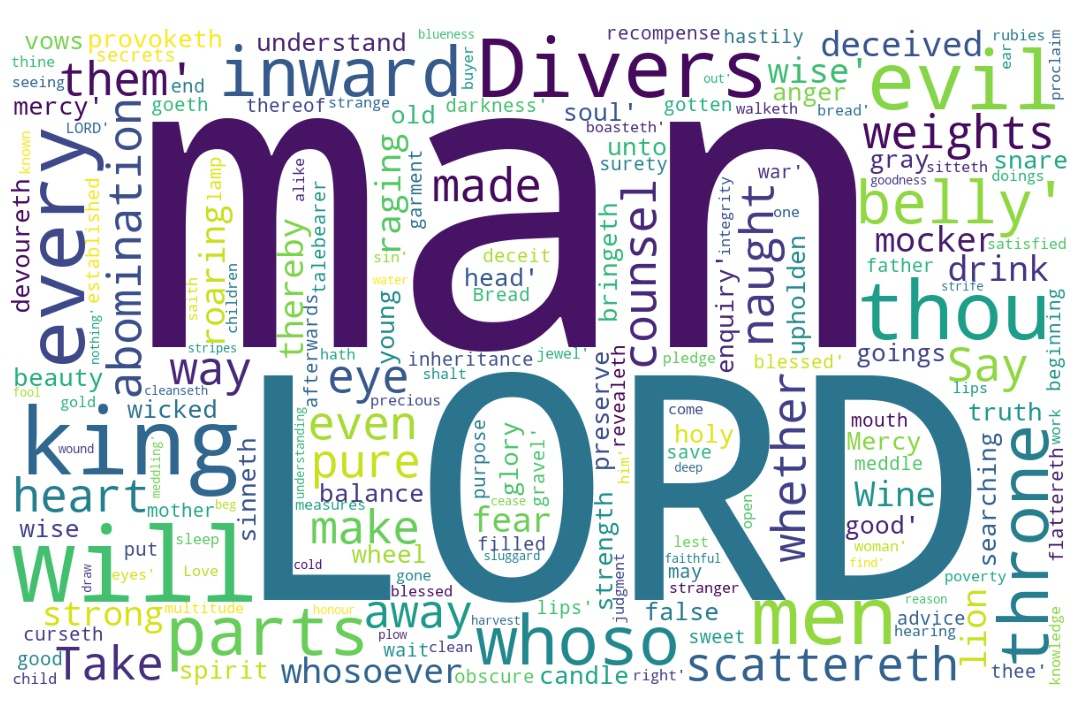
\includegraphics[width=\linewidth]{20OT-Proverbs/Proverb20-WordCloud.jpg}
  \caption{Proverb 20 Word Cloud}
  \label{fig:Proverb 20 word Cloud}
\end{figure}
\marginpar{\scriptsize \centering \fcolorbox{bone}{lime}{\textbf{PRINCIPLES TO OBSERVE}}\\ (Proverbs 20:1-30) \begin{compactenum}[I.][8]
    \item A \textbf{Fool and His Wine} \index[scripture]{Proverbs!Pro 20:01} (Pro 20:1)
    \item The \textbf{Fear of the King} \index[scripture]{Proverbs!Pro 20:02} (Pro 20:2) -- pay attention to those who can help you and those who can hurt you!
    \item \textbf{Fields Unplowed} \index[scripture]{Proverbs!Pro 20:04} (Pro 20:4) -- the bill for neglect comes with interest!
    \item The \textbf{Faithful Man Unseen} \index[scripture]{Proverbs!Pro 20:06} (Pro 20:6) -- when you find someone faithful (like a friend) hang on to that one
    \item \textbf{Finding Things out (with God's Help)} \index[scripture]{Proverbs!Pro 20:12} (Pro 20:12)
    \item The \textbf{Flatterer to Avoid} \index[scripture]{Proverbs!Pro 20:19} (Pro 20:19)
    \item The \textbf{False Balance Decried} \index[scripture]{Proverbs!Pro 20:23} (Pro 20:23) -- treat things with equity
\end{compactenum}}

\marginpar{\scriptsize \centering \fcolorbox{bone}{yellow}{\textbf{THE WORKS OF THE FOOL}}\\ (Proverbs 20:1-30) \begin{compactenum}[I.][8]
    \item Loses \textbf{Inhibitions} \index[scripture]{Proverbs!Pro 20:01} (Pro 20:1)
    \item Becomes an \textbf{Instigator} \index[scripture]{Proverbs!Pro 20:03} (Pro 20:3)
    \item Loves \textbf{Inactivity} \index[scripture]{Proverbs!Pro 20:04} (Pro 20:4)
    \item Possesses No \textbf{Integity} \index[scripture]{Proverbs!Pro 20:07} (Pro 20:7)
    \item Shows \textbf{Insincerity} \index[scripture]{Proverbs!Pro 20:19} (Pro 20:19)
    \item Has \textbf{Ingratitude} \index[scripture]{Proverbs!Pro 20:20} (Pro 20:20)
    \item Never Practices \textbf{Introspection} \index[scripture]{Proverbs!Pro 20:27} (Pro 20:27)
\end{compactenum}}

\footnote{\textcolor[cmyk]{0.99998,1,0,0}{\hyperlink{TOC}{Return to end of Table of Contents.}}}\footnote{\href{https://audiobible.com/bible/proverbs_20.html}{\textcolor[cmyk]{0.99998,1,0,0}{Proverbs Audio}}}\textcolor[cmyk]{0.99998,1,0,0}{Wine \emph{is} a mocker, strong drink \emph{is} raging: and \fcolorbox{bone}{lime}{whosoever is deceived} thereby is not wise.}
[2] \textcolor[cmyk]{0.99998,1,0,0}{The \fcolorbox{bone}{lime}{fear of a king} \emph{is} as the roaring of a lion: \emph{whoso} provoketh him to anger sinneth \emph{against} his own soul.}
[3] \textcolor[cmyk]{0.99998,1,0,0}{\emph{It} \emph{is} an honour for a man to cease from strife: but every fool will be meddling.}
[4] \textcolor[cmyk]{0.99998,1,0,0}{The sluggard \fcolorbox{bone}{lime}{will not plow} by reason of the cold; \emph{therefore} shall he beg in harvest, and \emph{have} nothing.}
[5] \textcolor[cmyk]{0.99998,1,0,0}{Counsel in the heart of man \emph{is} \emph{like} deep water; but a man of \fcolorbox{bone}{MYGOLD}{understanding} will draw it out.}
[6] \textcolor[cmyk]{0.99998,1,0,0}{Most men will proclaim every one his own goodness: but a \fcolorbox{bone}{lime}{faithful man} who can find?}
[7] \textcolor[cmyk]{0.99998,1,0,0}{The just \emph{man} walketh in his integrity: his children \emph{are} blessed after him.}
[8] \textcolor[cmyk]{0.99998,1,0,0}{A king that sitteth in the throne of judgment scattereth away all evil with his eyes.}
[9] \textcolor[cmyk]{0.99998,1,0,0}{Who can say, I have made my heart clean, I am pure from my sin?}
[10] \textcolor[cmyk]{0.99998,1,0,0}{Divers weights, \emph{and} divers measures, both of them \emph{are} alike abomination to the LORD.}
[11] \textcolor[cmyk]{0.99998,1,0,0}{Even a child is known by his doings, whether his work \emph{be} pure, and whether \emph{it} \emph{be} right.}
[12] \textcolor[cmyk]{0.99998,1,0,0}{The \fcolorbox{bone}{lime}{hearing ear}, and the \fcolorbox{bone}{lime}{seeing eye}, the LORD hath made even both of them.}\footnote{\textbf{Proverb 25:2} - It is the glory of God to conceal a thing: but the honour of kings is to search out a matter.}
[13] \textcolor[cmyk]{0.99998,1,0,0}{Love not sleep, lest thou come to poverty; open thine eyes, \emph{and} thou shalt be satisfied with bread.}
[14] \textcolor[cmyk]{0.99998,1,0,0}{\emph{It} \emph{is} naught, \emph{it} \emph{is} naught, saith the buyer: but when he is gone his way, then he boasteth.}
[15] \textcolor[cmyk]{0.99998,1,0,0}{There is gold, and a multitude of rubies: but the lips of knowledge \emph{are} a precious jewel.}
[16] \textcolor[cmyk]{0.99998,1,0,0}{Take his garment that is surety \emph{for} a stranger: and take a pledge of him for a strange woman.}
[17] \textcolor[cmyk]{0.99998,1,0,0}{Bread of deceit \emph{is} sweet to a man; but afterwards his mouth shall be filled with gravel.}
[18] \textcolor[cmyk]{0.99998,1,0,0}{\emph{Every} purpose is established by counsel: and with good advice make war.}
[19] \textcolor[cmyk]{0.99998,1,0,0}{He that goeth about \emph{as} a talebearer revealeth secrets: therefore meddle not with him that \fcolorbox{bone}{lime}{flattereth} with his lips.}
[20] \textcolor[cmyk]{0.99998,1,0,0}{Whoso curseth his father or his mother, his lamp shall be put out in obscure darkness.}
[21] \textcolor[cmyk]{0.99998,1,0,0}{An inheritance \emph{may} \emph{be} gotten hastily at the beginning; but the end thereof shall not be blessed.}
[22] \textcolor[cmyk]{0.99998,1,0,0}{Say not thou, I will recompense evil; \emph{but} wait on the LORD, and he shall save thee.}
[23] \textcolor[cmyk]{0.99998,1,0,0}{Divers weights \emph{are} an abomination unto the LORD; and a \fcolorbox{bone}{lime}{false balance} \emph{is} not good.}
[24] \textcolor[cmyk]{0.99998,1,0,0}{Man's goings \emph{are} of the LORD; how can a man then understand his own way?}\footnote{\textbf{Jeremiah 17:9,10} - The heart is deceitful above all things, and desperately wicked: who can know it? [10] I the LORD search the heart, I try the reins, even to give every man according to his ways, and according to the fruit of his doings.}
[25] \textcolor[cmyk]{0.99998,1,0,0}{\emph{It} \emph{is} a snare to the man \emph{who} devoureth \emph{that} \emph{which} \emph{is} holy, and after vows to make enquiry.}
[26] \textcolor[cmyk]{0.99998,1,0,0}{A wise king scattereth the wicked, and bringeth the wheel over them.}
[27] \textcolor[cmyk]{0.99998,1,0,0}{The spirit of man \emph{is} the candle of the LORD, searching all the inward parts of the belly.}
[28] \textcolor[cmyk]{0.99998,1,0,0}{Mercy and truth preserve the king: and his throne is upholden by mercy.}
[29] \textcolor[cmyk]{0.99998,1,0,0}{The glory of young men \emph{is} their strength: and the beauty of old men \emph{is} the gray head.}
[30] \textcolor[cmyk]{0.99998,1,0,0}{The blueness of a wound cleanseth away evil: so \emph{do} stripes the inward parts of the belly.}




\index[NWIV]{16!Proverbs!Pro 20:1}\index[AWIP]{Wine!Proverbs!Pro 20:1}\index[AWIP]{\emph{is}!Proverbs!Pro 20:1}\index[AWIP]{\emph{is}!Proverbs!Pro 20:1 (2)}\index[AWIP]{a!Proverbs!Pro 20:1}\index[AWIP]{mocker!Proverbs!Pro 20:1}\index[AWIP]{strong!Proverbs!Pro 20:1}\index[AWIP]{drink!Proverbs!Pro 20:1}\index[AWIP]{raging!Proverbs!Pro 20:1}\index[AWIP]{and!Proverbs!Pro 20:1}\index[AWIP]{whosoever!Proverbs!Pro 20:1}\index[AWIP]{is!Proverbs!Pro 20:1}\index[AWIP]{is!Proverbs!Pro 20:1 (2)}\index[AWIP]{deceived!Proverbs!Pro 20:1}\index[AWIP]{thereby!Proverbs!Pro 20:1}\index[AWIP]{not!Proverbs!Pro 20:1}\index[AWIP]{wise!Proverbs!Pro 20:1}\index[AWIP]{\emph{is}!Proverbs!Pro 20:1}\index[AWIP]{\emph{is}!Proverbs!Pro 20:1 (2)}

\index[NWIV]{22!Proverbs!Pro 20:2}\index[AWIP]{The!Proverbs!Pro 20:2}\index[AWIP]{fear!Proverbs!Pro 20:2}\index[AWIP]{of!Proverbs!Pro 20:2}\index[AWIP]{of!Proverbs!Pro 20:2 (2)}\index[AWIP]{a!Proverbs!Pro 20:2}\index[AWIP]{a!Proverbs!Pro 20:2 (2)}\index[AWIP]{king!Proverbs!Pro 20:2}\index[AWIP]{\emph{is}!Proverbs!Pro 20:2}\index[AWIP]{as!Proverbs!Pro 20:2}\index[AWIP]{the!Proverbs!Pro 20:2}\index[AWIP]{roaring!Proverbs!Pro 20:2}\index[AWIP]{lion!Proverbs!Pro 20:2}\index[AWIP]{\emph{whoso}!Proverbs!Pro 20:2}\index[AWIP]{provoketh!Proverbs!Pro 20:2}\index[AWIP]{him!Proverbs!Pro 20:2}\index[AWIP]{to!Proverbs!Pro 20:2}\index[AWIP]{anger!Proverbs!Pro 20:2}\index[AWIP]{sinneth!Proverbs!Pro 20:2}\index[AWIP]{\emph{against}!Proverbs!Pro 20:2}\index[AWIP]{his!Proverbs!Pro 20:2}\index[AWIP]{own!Proverbs!Pro 20:2}\index[AWIP]{soul!Proverbs!Pro 20:2}\index[AWIP]{\emph{is}!Proverbs!Pro 20:2}\index[AWIP]{\emph{whoso}!Proverbs!Pro 20:2}\index[AWIP]{\emph{against}!Proverbs!Pro 20:2}

\index[NWIV]{17!Proverbs!Pro 20:3}\index[AWIP]{\emph{It}!Proverbs!Pro 20:3}\index[AWIP]{\emph{is}!Proverbs!Pro 20:3}\index[AWIP]{an!Proverbs!Pro 20:3}\index[AWIP]{honour!Proverbs!Pro 20:3}\index[AWIP]{for!Proverbs!Pro 20:3}\index[AWIP]{a!Proverbs!Pro 20:3}\index[AWIP]{man!Proverbs!Pro 20:3}\index[AWIP]{to!Proverbs!Pro 20:3}\index[AWIP]{cease!Proverbs!Pro 20:3}\index[AWIP]{from!Proverbs!Pro 20:3}\index[AWIP]{strife!Proverbs!Pro 20:3}\index[AWIP]{but!Proverbs!Pro 20:3}\index[AWIP]{every!Proverbs!Pro 20:3}\index[AWIP]{fool!Proverbs!Pro 20:3}\index[AWIP]{will!Proverbs!Pro 20:3}\index[AWIP]{be!Proverbs!Pro 20:3}\index[AWIP]{meddling!Proverbs!Pro 20:3}\index[AWIP]{\emph{It}!Proverbs!Pro 20:3}\index[AWIP]{\emph{is}!Proverbs!Pro 20:3}

\index[NWIV]{19!Proverbs!Pro 20:4}\index[AWIP]{The!Proverbs!Pro 20:4}\index[AWIP]{sluggard!Proverbs!Pro 20:4}\index[AWIP]{will!Proverbs!Pro 20:4}\index[AWIP]{not!Proverbs!Pro 20:4}\index[AWIP]{plow!Proverbs!Pro 20:4}\index[AWIP]{by!Proverbs!Pro 20:4}\index[AWIP]{reason!Proverbs!Pro 20:4}\index[AWIP]{of!Proverbs!Pro 20:4}\index[AWIP]{the!Proverbs!Pro 20:4}\index[AWIP]{cold!Proverbs!Pro 20:4}\index[AWIP]{\emph{therefore}!Proverbs!Pro 20:4}\index[AWIP]{shall!Proverbs!Pro 20:4}\index[AWIP]{he!Proverbs!Pro 20:4}\index[AWIP]{beg!Proverbs!Pro 20:4}\index[AWIP]{in!Proverbs!Pro 20:4}\index[AWIP]{harvest!Proverbs!Pro 20:4}\index[AWIP]{and!Proverbs!Pro 20:4}\index[AWIP]{\emph{have}!Proverbs!Pro 20:4}\index[AWIP]{nothing!Proverbs!Pro 20:4}\index[AWIP]{\emph{therefore}!Proverbs!Pro 20:4}\index[AWIP]{\emph{have}!Proverbs!Pro 20:4}

\index[NWIV]{19!Proverbs!Pro 20:5}\index[AWIP]{Counsel!Proverbs!Pro 20:5}\index[AWIP]{in!Proverbs!Pro 20:5}\index[AWIP]{the!Proverbs!Pro 20:5}\index[AWIP]{heart!Proverbs!Pro 20:5}\index[AWIP]{of!Proverbs!Pro 20:5}\index[AWIP]{of!Proverbs!Pro 20:5 (2)}\index[AWIP]{man!Proverbs!Pro 20:5}\index[AWIP]{man!Proverbs!Pro 20:5 (2)}\index[AWIP]{\emph{is}!Proverbs!Pro 20:5}\index[AWIP]{\emph{like}!Proverbs!Pro 20:5}\index[AWIP]{deep!Proverbs!Pro 20:5}\index[AWIP]{water!Proverbs!Pro 20:5}\index[AWIP]{but!Proverbs!Pro 20:5}\index[AWIP]{a!Proverbs!Pro 20:5}\index[AWIP]{understanding!Proverbs!Pro 20:5}\index[AWIP]{will!Proverbs!Pro 20:5}\index[AWIP]{draw!Proverbs!Pro 20:5}\index[AWIP]{it!Proverbs!Pro 20:5}\index[AWIP]{out!Proverbs!Pro 20:5}\index[AWIP]{\emph{is}!Proverbs!Pro 20:5}\index[AWIP]{\emph{like}!Proverbs!Pro 20:5}

\index[NWIV]{16!Proverbs!Pro 20:6}\index[AWIP]{Most!Proverbs!Pro 20:6}\index[AWIP]{men!Proverbs!Pro 20:6}\index[AWIP]{will!Proverbs!Pro 20:6}\index[AWIP]{proclaim!Proverbs!Pro 20:6}\index[AWIP]{every!Proverbs!Pro 20:6}\index[AWIP]{one!Proverbs!Pro 20:6}\index[AWIP]{his!Proverbs!Pro 20:6}\index[AWIP]{own!Proverbs!Pro 20:6}\index[AWIP]{goodness!Proverbs!Pro 20:6}\index[AWIP]{but!Proverbs!Pro 20:6}\index[AWIP]{a!Proverbs!Pro 20:6}\index[AWIP]{faithful!Proverbs!Pro 20:6}\index[AWIP]{man!Proverbs!Pro 20:6}\index[AWIP]{who!Proverbs!Pro 20:6}\index[AWIP]{can!Proverbs!Pro 20:6}\index[AWIP]{find?!Proverbs!Pro 20:6}

\index[NWIV]{13!Proverbs!Pro 20:7}\index[AWIP]{The!Proverbs!Pro 20:7}\index[AWIP]{just!Proverbs!Pro 20:7}\index[AWIP]{\emph{man}!Proverbs!Pro 20:7}\index[AWIP]{walketh!Proverbs!Pro 20:7}\index[AWIP]{in!Proverbs!Pro 20:7}\index[AWIP]{his!Proverbs!Pro 20:7}\index[AWIP]{his!Proverbs!Pro 20:7 (2)}\index[AWIP]{integrity!Proverbs!Pro 20:7}\index[AWIP]{children!Proverbs!Pro 20:7}\index[AWIP]{\emph{are}!Proverbs!Pro 20:7}\index[AWIP]{blessed!Proverbs!Pro 20:7}\index[AWIP]{after!Proverbs!Pro 20:7}\index[AWIP]{him!Proverbs!Pro 20:7}\index[AWIP]{\emph{man}!Proverbs!Pro 20:7}\index[AWIP]{\emph{are}!Proverbs!Pro 20:7}

\index[NWIV]{16!Proverbs!Pro 20:8}\index[AWIP]{A!Proverbs!Pro 20:8}\index[AWIP]{king!Proverbs!Pro 20:8}\index[AWIP]{that!Proverbs!Pro 20:8}\index[AWIP]{sitteth!Proverbs!Pro 20:8}\index[AWIP]{in!Proverbs!Pro 20:8}\index[AWIP]{the!Proverbs!Pro 20:8}\index[AWIP]{throne!Proverbs!Pro 20:8}\index[AWIP]{of!Proverbs!Pro 20:8}\index[AWIP]{judgment!Proverbs!Pro 20:8}\index[AWIP]{scattereth!Proverbs!Pro 20:8}\index[AWIP]{away!Proverbs!Pro 20:8}\index[AWIP]{all!Proverbs!Pro 20:8}\index[AWIP]{evil!Proverbs!Pro 20:8}\index[AWIP]{with!Proverbs!Pro 20:8}\index[AWIP]{his!Proverbs!Pro 20:8}\index[AWIP]{eyes!Proverbs!Pro 20:8}

\index[NWIV]{15!Proverbs!Pro 20:9}\index[AWIP]{Who!Proverbs!Pro 20:9}\index[AWIP]{can!Proverbs!Pro 20:9}\index[AWIP]{say!Proverbs!Pro 20:9}\index[AWIP]{I!Proverbs!Pro 20:9}\index[AWIP]{I!Proverbs!Pro 20:9 (2)}\index[AWIP]{have!Proverbs!Pro 20:9}\index[AWIP]{made!Proverbs!Pro 20:9}\index[AWIP]{my!Proverbs!Pro 20:9}\index[AWIP]{my!Proverbs!Pro 20:9 (2)}\index[AWIP]{heart!Proverbs!Pro 20:9}\index[AWIP]{clean!Proverbs!Pro 20:9}\index[AWIP]{am!Proverbs!Pro 20:9}\index[AWIP]{pure!Proverbs!Pro 20:9}\index[AWIP]{from!Proverbs!Pro 20:9}\index[AWIP]{sin?!Proverbs!Pro 20:9}

\index[NWIV]{14!Proverbs!Pro 20:10}\index[AWIP]{Divers!Proverbs!Pro 20:10}\index[AWIP]{weights!Proverbs!Pro 20:10}\index[AWIP]{\emph{and}!Proverbs!Pro 20:10}\index[AWIP]{divers!Proverbs!Pro 20:10}\index[AWIP]{measures!Proverbs!Pro 20:10}\index[AWIP]{both!Proverbs!Pro 20:10}\index[AWIP]{of!Proverbs!Pro 20:10}\index[AWIP]{them!Proverbs!Pro 20:10}\index[AWIP]{\emph{are}!Proverbs!Pro 20:10}\index[AWIP]{alike!Proverbs!Pro 20:10}\index[AWIP]{abomination!Proverbs!Pro 20:10}\index[AWIP]{to!Proverbs!Pro 20:10}\index[AWIP]{the!Proverbs!Pro 20:10}\index[AWIP]{LORD!Proverbs!Pro 20:10}\index[AWIP]{\emph{and}!Proverbs!Pro 20:10}\index[AWIP]{\emph{are}!Proverbs!Pro 20:10}

\index[NWIV]{18!Proverbs!Pro 20:11}\index[AWIP]{Even!Proverbs!Pro 20:11}\index[AWIP]{a!Proverbs!Pro 20:11}\index[AWIP]{child!Proverbs!Pro 20:11}\index[AWIP]{is!Proverbs!Pro 20:11}\index[AWIP]{known!Proverbs!Pro 20:11}\index[AWIP]{by!Proverbs!Pro 20:11}\index[AWIP]{his!Proverbs!Pro 20:11}\index[AWIP]{his!Proverbs!Pro 20:11 (2)}\index[AWIP]{doings!Proverbs!Pro 20:11}\index[AWIP]{whether!Proverbs!Pro 20:11}\index[AWIP]{whether!Proverbs!Pro 20:11 (2)}\index[AWIP]{work!Proverbs!Pro 20:11}\index[AWIP]{\emph{be}!Proverbs!Pro 20:11}\index[AWIP]{\emph{be}!Proverbs!Pro 20:11 (2)}\index[AWIP]{pure!Proverbs!Pro 20:11}\index[AWIP]{and!Proverbs!Pro 20:11}\index[AWIP]{\emph{it}!Proverbs!Pro 20:11}\index[AWIP]{right!Proverbs!Pro 20:11}\index[AWIP]{\emph{be}!Proverbs!Pro 20:11}\index[AWIP]{\emph{be}!Proverbs!Pro 20:11 (2)}\index[AWIP]{\emph{it}!Proverbs!Pro 20:11}

\index[NWIV]{15!Proverbs!Pro 20:12}\index[AWIP]{The!Proverbs!Pro 20:12}\index[AWIP]{hearing!Proverbs!Pro 20:12}\index[AWIP]{ear!Proverbs!Pro 20:12}\index[AWIP]{and!Proverbs!Pro 20:12}\index[AWIP]{the!Proverbs!Pro 20:12}\index[AWIP]{the!Proverbs!Pro 20:12 (2)}\index[AWIP]{seeing!Proverbs!Pro 20:12}\index[AWIP]{eye!Proverbs!Pro 20:12}\index[AWIP]{LORD!Proverbs!Pro 20:12}\index[AWIP]{hath!Proverbs!Pro 20:12}\index[AWIP]{made!Proverbs!Pro 20:12}\index[AWIP]{even!Proverbs!Pro 20:12}\index[AWIP]{both!Proverbs!Pro 20:12}\index[AWIP]{of!Proverbs!Pro 20:12}\index[AWIP]{them!Proverbs!Pro 20:12}

\index[NWIV]{18!Proverbs!Pro 20:13}\index[AWIP]{Love!Proverbs!Pro 20:13}\index[AWIP]{not!Proverbs!Pro 20:13}\index[AWIP]{sleep!Proverbs!Pro 20:13}\index[AWIP]{lest!Proverbs!Pro 20:13}\index[AWIP]{thou!Proverbs!Pro 20:13}\index[AWIP]{thou!Proverbs!Pro 20:13 (2)}\index[AWIP]{come!Proverbs!Pro 20:13}\index[AWIP]{to!Proverbs!Pro 20:13}\index[AWIP]{poverty!Proverbs!Pro 20:13}\index[AWIP]{open!Proverbs!Pro 20:13}\index[AWIP]{thine!Proverbs!Pro 20:13}\index[AWIP]{eyes!Proverbs!Pro 20:13}\index[AWIP]{\emph{and}!Proverbs!Pro 20:13}\index[AWIP]{shalt!Proverbs!Pro 20:13}\index[AWIP]{be!Proverbs!Pro 20:13}\index[AWIP]{satisfied!Proverbs!Pro 20:13}\index[AWIP]{with!Proverbs!Pro 20:13}\index[AWIP]{bread!Proverbs!Pro 20:13}\index[AWIP]{\emph{and}!Proverbs!Pro 20:13}

\index[NWIV]{19!Proverbs!Pro 20:14}\index[AWIP]{\emph{It}!Proverbs!Pro 20:14}\index[AWIP]{\emph{is}!Proverbs!Pro 20:14}\index[AWIP]{\emph{is}!Proverbs!Pro 20:14 (2)}\index[AWIP]{naught!Proverbs!Pro 20:14}\index[AWIP]{naught!Proverbs!Pro 20:14 (2)}\index[AWIP]{\emph{it}!Proverbs!Pro 20:14}\index[AWIP]{saith!Proverbs!Pro 20:14}\index[AWIP]{the!Proverbs!Pro 20:14}\index[AWIP]{buyer!Proverbs!Pro 20:14}\index[AWIP]{but!Proverbs!Pro 20:14}\index[AWIP]{when!Proverbs!Pro 20:14}\index[AWIP]{he!Proverbs!Pro 20:14}\index[AWIP]{he!Proverbs!Pro 20:14 (2)}\index[AWIP]{is!Proverbs!Pro 20:14}\index[AWIP]{gone!Proverbs!Pro 20:14}\index[AWIP]{his!Proverbs!Pro 20:14}\index[AWIP]{way!Proverbs!Pro 20:14}\index[AWIP]{then!Proverbs!Pro 20:14}\index[AWIP]{boasteth!Proverbs!Pro 20:14}\index[AWIP]{\emph{It}!Proverbs!Pro 20:14}\index[AWIP]{\emph{is}!Proverbs!Pro 20:14}\index[AWIP]{\emph{is}!Proverbs!Pro 20:14 (2)}\index[AWIP]{\emph{it}!Proverbs!Pro 20:14}

\index[NWIV]{17!Proverbs!Pro 20:15}\index[AWIP]{There!Proverbs!Pro 20:15}\index[AWIP]{is!Proverbs!Pro 20:15}\index[AWIP]{gold!Proverbs!Pro 20:15}\index[AWIP]{and!Proverbs!Pro 20:15}\index[AWIP]{a!Proverbs!Pro 20:15}\index[AWIP]{a!Proverbs!Pro 20:15 (2)}\index[AWIP]{multitude!Proverbs!Pro 20:15}\index[AWIP]{of!Proverbs!Pro 20:15}\index[AWIP]{of!Proverbs!Pro 20:15 (2)}\index[AWIP]{rubies!Proverbs!Pro 20:15}\index[AWIP]{but!Proverbs!Pro 20:15}\index[AWIP]{the!Proverbs!Pro 20:15}\index[AWIP]{lips!Proverbs!Pro 20:15}\index[AWIP]{knowledge!Proverbs!Pro 20:15}\index[AWIP]{\emph{are}!Proverbs!Pro 20:15}\index[AWIP]{precious!Proverbs!Pro 20:15}\index[AWIP]{jewel!Proverbs!Pro 20:15}\index[AWIP]{\emph{are}!Proverbs!Pro 20:15}

\index[NWIV]{19!Proverbs!Pro 20:16}\index[AWIP]{Take!Proverbs!Pro 20:16}\index[AWIP]{his!Proverbs!Pro 20:16}\index[AWIP]{garment!Proverbs!Pro 20:16}\index[AWIP]{that!Proverbs!Pro 20:16}\index[AWIP]{is!Proverbs!Pro 20:16}\index[AWIP]{surety!Proverbs!Pro 20:16}\index[AWIP]{\emph{for}!Proverbs!Pro 20:16}\index[AWIP]{a!Proverbs!Pro 20:16}\index[AWIP]{a!Proverbs!Pro 20:16 (2)}\index[AWIP]{a!Proverbs!Pro 20:16 (3)}\index[AWIP]{stranger!Proverbs!Pro 20:16}\index[AWIP]{and!Proverbs!Pro 20:16}\index[AWIP]{take!Proverbs!Pro 20:16}\index[AWIP]{pledge!Proverbs!Pro 20:16}\index[AWIP]{of!Proverbs!Pro 20:16}\index[AWIP]{him!Proverbs!Pro 20:16}\index[AWIP]{for!Proverbs!Pro 20:16}\index[AWIP]{strange!Proverbs!Pro 20:16}\index[AWIP]{woman!Proverbs!Pro 20:16}\index[AWIP]{\emph{for}!Proverbs!Pro 20:16}

\index[NWIV]{17!Proverbs!Pro 20:17}\index[AWIP]{Bread!Proverbs!Pro 20:17}\index[AWIP]{of!Proverbs!Pro 20:17}\index[AWIP]{deceit!Proverbs!Pro 20:17}\index[AWIP]{\emph{is}!Proverbs!Pro 20:17}\index[AWIP]{sweet!Proverbs!Pro 20:17}\index[AWIP]{to!Proverbs!Pro 20:17}\index[AWIP]{a!Proverbs!Pro 20:17}\index[AWIP]{man!Proverbs!Pro 20:17}\index[AWIP]{but!Proverbs!Pro 20:17}\index[AWIP]{afterwards!Proverbs!Pro 20:17}\index[AWIP]{his!Proverbs!Pro 20:17}\index[AWIP]{mouth!Proverbs!Pro 20:17}\index[AWIP]{shall!Proverbs!Pro 20:17}\index[AWIP]{be!Proverbs!Pro 20:17}\index[AWIP]{filled!Proverbs!Pro 20:17}\index[AWIP]{with!Proverbs!Pro 20:17}\index[AWIP]{gravel!Proverbs!Pro 20:17}\index[AWIP]{\emph{is}!Proverbs!Pro 20:17}

\index[NWIV]{12!Proverbs!Pro 20:18}\index[AWIP]{\emph{Every}!Proverbs!Pro 20:18}\index[AWIP]{purpose!Proverbs!Pro 20:18}\index[AWIP]{is!Proverbs!Pro 20:18}\index[AWIP]{established!Proverbs!Pro 20:18}\index[AWIP]{by!Proverbs!Pro 20:18}\index[AWIP]{counsel!Proverbs!Pro 20:18}\index[AWIP]{and!Proverbs!Pro 20:18}\index[AWIP]{with!Proverbs!Pro 20:18}\index[AWIP]{good!Proverbs!Pro 20:18}\index[AWIP]{advice!Proverbs!Pro 20:18}\index[AWIP]{make!Proverbs!Pro 20:18}\index[AWIP]{war!Proverbs!Pro 20:18}\index[AWIP]{\emph{Every}!Proverbs!Pro 20:18}

\index[NWIV]{19!Proverbs!Pro 20:19}\index[AWIP]{He!Proverbs!Pro 20:19}\index[AWIP]{that!Proverbs!Pro 20:19}\index[AWIP]{that!Proverbs!Pro 20:19 (2)}\index[AWIP]{goeth!Proverbs!Pro 20:19}\index[AWIP]{about!Proverbs!Pro 20:19}\index[AWIP]{\emph{as}!Proverbs!Pro 20:19}\index[AWIP]{a!Proverbs!Pro 20:19}\index[AWIP]{talebearer!Proverbs!Pro 20:19}\index[AWIP]{revealeth!Proverbs!Pro 20:19}\index[AWIP]{secrets!Proverbs!Pro 20:19}\index[AWIP]{therefore!Proverbs!Pro 20:19}\index[AWIP]{meddle!Proverbs!Pro 20:19}\index[AWIP]{not!Proverbs!Pro 20:19}\index[AWIP]{with!Proverbs!Pro 20:19}\index[AWIP]{with!Proverbs!Pro 20:19 (2)}\index[AWIP]{him!Proverbs!Pro 20:19}\index[AWIP]{flattereth!Proverbs!Pro 20:19}\index[AWIP]{his!Proverbs!Pro 20:19}\index[AWIP]{lips!Proverbs!Pro 20:19}\index[AWIP]{\emph{as}!Proverbs!Pro 20:19}

\index[NWIV]{16!Proverbs!Pro 20:20}\index[AWIP]{Whoso!Proverbs!Pro 20:20}\index[AWIP]{curseth!Proverbs!Pro 20:20}\index[AWIP]{his!Proverbs!Pro 20:20}\index[AWIP]{his!Proverbs!Pro 20:20 (2)}\index[AWIP]{his!Proverbs!Pro 20:20 (3)}\index[AWIP]{father!Proverbs!Pro 20:20}\index[AWIP]{or!Proverbs!Pro 20:20}\index[AWIP]{mother!Proverbs!Pro 20:20}\index[AWIP]{lamp!Proverbs!Pro 20:20}\index[AWIP]{shall!Proverbs!Pro 20:20}\index[AWIP]{be!Proverbs!Pro 20:20}\index[AWIP]{put!Proverbs!Pro 20:20}\index[AWIP]{out!Proverbs!Pro 20:20}\index[AWIP]{in!Proverbs!Pro 20:20}\index[AWIP]{obscure!Proverbs!Pro 20:20}\index[AWIP]{darkness!Proverbs!Pro 20:20}

\index[NWIV]{17!Proverbs!Pro 20:21}\index[AWIP]{An!Proverbs!Pro 20:21}\index[AWIP]{inheritance!Proverbs!Pro 20:21}\index[AWIP]{\emph{may}!Proverbs!Pro 20:21}\index[AWIP]{\emph{be}!Proverbs!Pro 20:21}\index[AWIP]{gotten!Proverbs!Pro 20:21}\index[AWIP]{hastily!Proverbs!Pro 20:21}\index[AWIP]{at!Proverbs!Pro 20:21}\index[AWIP]{the!Proverbs!Pro 20:21}\index[AWIP]{the!Proverbs!Pro 20:21 (2)}\index[AWIP]{beginning!Proverbs!Pro 20:21}\index[AWIP]{but!Proverbs!Pro 20:21}\index[AWIP]{end!Proverbs!Pro 20:21}\index[AWIP]{thereof!Proverbs!Pro 20:21}\index[AWIP]{shall!Proverbs!Pro 20:21}\index[AWIP]{not!Proverbs!Pro 20:21}\index[AWIP]{be!Proverbs!Pro 20:21}\index[AWIP]{blessed!Proverbs!Pro 20:21}\index[AWIP]{\emph{may}!Proverbs!Pro 20:21}\index[AWIP]{\emph{be}!Proverbs!Pro 20:21}

\index[NWIV]{17!Proverbs!Pro 20:22}\index[AWIP]{Say!Proverbs!Pro 20:22}\index[AWIP]{not!Proverbs!Pro 20:22}\index[AWIP]{thou!Proverbs!Pro 20:22}\index[AWIP]{I!Proverbs!Pro 20:22}\index[AWIP]{will!Proverbs!Pro 20:22}\index[AWIP]{recompense!Proverbs!Pro 20:22}\index[AWIP]{evil!Proverbs!Pro 20:22}\index[AWIP]{\emph{but}!Proverbs!Pro 20:22}\index[AWIP]{wait!Proverbs!Pro 20:22}\index[AWIP]{on!Proverbs!Pro 20:22}\index[AWIP]{the!Proverbs!Pro 20:22}\index[AWIP]{LORD!Proverbs!Pro 20:22}\index[AWIP]{and!Proverbs!Pro 20:22}\index[AWIP]{he!Proverbs!Pro 20:22}\index[AWIP]{shall!Proverbs!Pro 20:22}\index[AWIP]{save!Proverbs!Pro 20:22}\index[AWIP]{thee!Proverbs!Pro 20:22}\index[AWIP]{\emph{but}!Proverbs!Pro 20:22}

\index[NWIV]{15!Proverbs!Pro 20:23}\index[AWIP]{Divers!Proverbs!Pro 20:23}\index[AWIP]{weights!Proverbs!Pro 20:23}\index[AWIP]{\emph{are}!Proverbs!Pro 20:23}\index[AWIP]{an!Proverbs!Pro 20:23}\index[AWIP]{abomination!Proverbs!Pro 20:23}\index[AWIP]{unto!Proverbs!Pro 20:23}\index[AWIP]{the!Proverbs!Pro 20:23}\index[AWIP]{LORD!Proverbs!Pro 20:23}\index[AWIP]{and!Proverbs!Pro 20:23}\index[AWIP]{a!Proverbs!Pro 20:23}\index[AWIP]{false!Proverbs!Pro 20:23}\index[AWIP]{balance!Proverbs!Pro 20:23}\index[AWIP]{\emph{is}!Proverbs!Pro 20:23}\index[AWIP]{not!Proverbs!Pro 20:23}\index[AWIP]{good!Proverbs!Pro 20:23}\index[AWIP]{\emph{are}!Proverbs!Pro 20:23}\index[AWIP]{\emph{is}!Proverbs!Pro 20:23}

\index[NWIV]{15!Proverbs!Pro 20:24}\index[AWIP]{Man's!Proverbs!Pro 20:24}\index[AWIP]{goings!Proverbs!Pro 20:24}\index[AWIP]{\emph{are}!Proverbs!Pro 20:24}\index[AWIP]{of!Proverbs!Pro 20:24}\index[AWIP]{the!Proverbs!Pro 20:24}\index[AWIP]{LORD!Proverbs!Pro 20:24}\index[AWIP]{how!Proverbs!Pro 20:24}\index[AWIP]{can!Proverbs!Pro 20:24}\index[AWIP]{a!Proverbs!Pro 20:24}\index[AWIP]{man!Proverbs!Pro 20:24}\index[AWIP]{then!Proverbs!Pro 20:24}\index[AWIP]{understand!Proverbs!Pro 20:24}\index[AWIP]{his!Proverbs!Pro 20:24}\index[AWIP]{own!Proverbs!Pro 20:24}\index[AWIP]{way?!Proverbs!Pro 20:24}\index[AWIP]{\emph{are}!Proverbs!Pro 20:24}

\index[NWIV]{19!Proverbs!Pro 20:25}\index[AWIP]{\emph{It}!Proverbs!Pro 20:25}\index[AWIP]{\emph{is}!Proverbs!Pro 20:25}\index[AWIP]{\emph{is}!Proverbs!Pro 20:25 (2)}\index[AWIP]{a!Proverbs!Pro 20:25}\index[AWIP]{snare!Proverbs!Pro 20:25}\index[AWIP]{to!Proverbs!Pro 20:25}\index[AWIP]{to!Proverbs!Pro 20:25 (2)}\index[AWIP]{the!Proverbs!Pro 20:25}\index[AWIP]{man!Proverbs!Pro 20:25}\index[AWIP]{\emph{who}!Proverbs!Pro 20:25}\index[AWIP]{devoureth!Proverbs!Pro 20:25}\index[AWIP]{\emph{that}!Proverbs!Pro 20:25}\index[AWIP]{\emph{which}!Proverbs!Pro 20:25}\index[AWIP]{holy!Proverbs!Pro 20:25}\index[AWIP]{and!Proverbs!Pro 20:25}\index[AWIP]{after!Proverbs!Pro 20:25}\index[AWIP]{vows!Proverbs!Pro 20:25}\index[AWIP]{make!Proverbs!Pro 20:25}\index[AWIP]{enquiry!Proverbs!Pro 20:25}\index[AWIP]{\emph{It}!Proverbs!Pro 20:25}\index[AWIP]{\emph{is}!Proverbs!Pro 20:25}\index[AWIP]{\emph{is}!Proverbs!Pro 20:25 (2)}\index[AWIP]{\emph{who}!Proverbs!Pro 20:25}\index[AWIP]{\emph{that}!Proverbs!Pro 20:25}\index[AWIP]{\emph{which}!Proverbs!Pro 20:25}

\index[NWIV]{12!Proverbs!Pro 20:26}\index[AWIP]{A!Proverbs!Pro 20:26}\index[AWIP]{wise!Proverbs!Pro 20:26}\index[AWIP]{king!Proverbs!Pro 20:26}\index[AWIP]{scattereth!Proverbs!Pro 20:26}\index[AWIP]{the!Proverbs!Pro 20:26}\index[AWIP]{the!Proverbs!Pro 20:26 (2)}\index[AWIP]{wicked!Proverbs!Pro 20:26}\index[AWIP]{and!Proverbs!Pro 20:26}\index[AWIP]{bringeth!Proverbs!Pro 20:26}\index[AWIP]{wheel!Proverbs!Pro 20:26}\index[AWIP]{over!Proverbs!Pro 20:26}\index[AWIP]{them!Proverbs!Pro 20:26}

\index[NWIV]{18!Proverbs!Pro 20:27}\index[AWIP]{The!Proverbs!Pro 20:27}\index[AWIP]{spirit!Proverbs!Pro 20:27}\index[AWIP]{of!Proverbs!Pro 20:27}\index[AWIP]{of!Proverbs!Pro 20:27 (2)}\index[AWIP]{of!Proverbs!Pro 20:27 (3)}\index[AWIP]{man!Proverbs!Pro 20:27}\index[AWIP]{\emph{is}!Proverbs!Pro 20:27}\index[AWIP]{the!Proverbs!Pro 20:27}\index[AWIP]{the!Proverbs!Pro 20:27 (2)}\index[AWIP]{the!Proverbs!Pro 20:27 (3)}\index[AWIP]{the!Proverbs!Pro 20:27 (4)}\index[AWIP]{candle!Proverbs!Pro 20:27}\index[AWIP]{LORD!Proverbs!Pro 20:27}\index[AWIP]{searching!Proverbs!Pro 20:27}\index[AWIP]{all!Proverbs!Pro 20:27}\index[AWIP]{inward!Proverbs!Pro 20:27}\index[AWIP]{parts!Proverbs!Pro 20:27}\index[AWIP]{belly!Proverbs!Pro 20:27}\index[AWIP]{\emph{is}!Proverbs!Pro 20:27}

\index[NWIV]{13!Proverbs!Pro 20:28}\index[AWIP]{Mercy!Proverbs!Pro 20:28}\index[AWIP]{and!Proverbs!Pro 20:28}\index[AWIP]{and!Proverbs!Pro 20:28 (2)}\index[AWIP]{truth!Proverbs!Pro 20:28}\index[AWIP]{preserve!Proverbs!Pro 20:28}\index[AWIP]{the!Proverbs!Pro 20:28}\index[AWIP]{king!Proverbs!Pro 20:28}\index[AWIP]{his!Proverbs!Pro 20:28}\index[AWIP]{throne!Proverbs!Pro 20:28}\index[AWIP]{is!Proverbs!Pro 20:28}\index[AWIP]{upholden!Proverbs!Pro 20:28}\index[AWIP]{by!Proverbs!Pro 20:28}\index[AWIP]{mercy!Proverbs!Pro 20:28}

\index[NWIV]{18!Proverbs!Pro 20:29}\index[AWIP]{The!Proverbs!Pro 20:29}\index[AWIP]{glory!Proverbs!Pro 20:29}\index[AWIP]{of!Proverbs!Pro 20:29}\index[AWIP]{of!Proverbs!Pro 20:29 (2)}\index[AWIP]{young!Proverbs!Pro 20:29}\index[AWIP]{men!Proverbs!Pro 20:29}\index[AWIP]{men!Proverbs!Pro 20:29 (2)}\index[AWIP]{\emph{is}!Proverbs!Pro 20:29}\index[AWIP]{\emph{is}!Proverbs!Pro 20:29 (2)}\index[AWIP]{their!Proverbs!Pro 20:29}\index[AWIP]{strength!Proverbs!Pro 20:29}\index[AWIP]{and!Proverbs!Pro 20:29}\index[AWIP]{the!Proverbs!Pro 20:29}\index[AWIP]{the!Proverbs!Pro 20:29 (2)}\index[AWIP]{beauty!Proverbs!Pro 20:29}\index[AWIP]{old!Proverbs!Pro 20:29}\index[AWIP]{gray!Proverbs!Pro 20:29}\index[AWIP]{head!Proverbs!Pro 20:29}\index[AWIP]{\emph{is}!Proverbs!Pro 20:29}\index[AWIP]{\emph{is}!Proverbs!Pro 20:29 (2)}

\index[NWIV]{17!Proverbs!Pro 20:30}\index[AWIP]{The!Proverbs!Pro 20:30}\index[AWIP]{blueness!Proverbs!Pro 20:30}\index[AWIP]{of!Proverbs!Pro 20:30}\index[AWIP]{of!Proverbs!Pro 20:30 (2)}\index[AWIP]{a!Proverbs!Pro 20:30}\index[AWIP]{wound!Proverbs!Pro 20:30}\index[AWIP]{cleanseth!Proverbs!Pro 20:30}\index[AWIP]{away!Proverbs!Pro 20:30}\index[AWIP]{evil!Proverbs!Pro 20:30}\index[AWIP]{so!Proverbs!Pro 20:30}\index[AWIP]{\emph{do}!Proverbs!Pro 20:30}\index[AWIP]{stripes!Proverbs!Pro 20:30}\index[AWIP]{the!Proverbs!Pro 20:30}\index[AWIP]{the!Proverbs!Pro 20:30 (2)}\index[AWIP]{inward!Proverbs!Pro 20:30}\index[AWIP]{parts!Proverbs!Pro 20:30}\index[AWIP]{belly!Proverbs!Pro 20:30}\index[AWIP]{\emph{do}!Proverbs!Pro 20:30}

%%%%%%%%%%%%%%%%%%%%%%%%%%%
%%%%%%%%%%%%%%%%%%%%%%%%%%%

\index[DOCTRINES]{Practicology - Sobriety!Proverbs!Pro 20:1}

\index[DOCTRINES]{Practicology - Standards!Proverbs!Pro 20:10}

\index[DOCTRINES]{Practicology - Secrecy!Proverbs!Pro 20:19}
\index[DOCTRINES]{Practicology - Secrecy!Proverbs!Pro 20:23}

\index[DOCTRINES]{Practicology - Stripes!Proverbs!Pro 20:30}




\section{Proverb 20 Outlines}

\subsection{My Outlines}

\subsubsection{Principles to Observe}

\index[speaker]{Keith Anthony!Proverb 20 (Principles to Observe)}
\index[series]{Proverbs (Keith Anthony)!Pro 20 (Principles to Observe)}
\index[date]{2016/05/20!Proverb 20 (Principles to Observe) (Keith Anthony)}
\begin{compactenum}[I.]
    \item A \textbf{Fool and His Wine} \index[scripture]{Proverbs!Pro 20:01} (Pro 20:1)
    \item The \textbf{Fear of the King} \index[scripture]{Proverbs!Pro 20:02} (Pro 20:2) -- pay attention to those who can help you and those who can hurt you!
    \item \textbf{Fields Unplowed} \index[scripture]{Proverbs!Pro 20:04} (Pro 20:4) -- the bill for neglect comes with interest!
    \item The \textbf{Faithful Man Unseen} \index[scripture]{Proverbs!Pro 20:06} (Pro 20:6) -- when you find someone faithful (like a friend) hang on to hat one
    \item \textbf{Finding Things out (with God's Help)} \index[scripture]{Proverbs!Pro 20:12} (Pro 20:12)
    \item The \textbf{Flatterer to Avoid} \index[scripture]{Proverbs!Pro 20:19} (Pro 20:19)
    \item The \textbf{False Balance Decried} \index[scripture]{Proverbs!Pro 20:23} (Pro 20:23) -- treat things with equity
\end{compactenum}


\subsubsection{The Works of the Fool}


\index[speaker]{Keith Anthony!Proverb 20 (The Works of the Fool)}
\index[series]{Proverbs (Keith Anthony)!Pro 20 (The Works of the Fool)}
\index[date]{2014/11/20!Proverb 20 (The Works of the Fool) (Keith Anthony)}

\begin{compactenum}[I.][8]
    \item Loses \textbf{Inhibitions} \index[scripture]{Proverbs!Pro 20:01} (Pro 20:1)
    \item Becomes an \textbf{Instigator} \index[scripture]{Proverbs!Pro 20:03} (Pro 20:3)
    \item Loves \textbf{Inactivity} \index[scripture]{Proverbs!Pro 20:04} (Pro 20:4)
    \item Possesses No \textbf{Integity} \index[scripture]{Proverbs!Pro 20:07} (Pro 20:7)
    \item Shows \textbf{Insincerity} \index[scripture]{Proverbs!Pro 20:19} (Pro 20:19)
    \item Has \textbf{Ingratitude} \index[scripture]{Proverbs!Pro 20:20} (Pro 20:20)
    \item Never Practices \textbf{Introspection} \index[scripture]{Proverbs!Pro 20:27} (Pro 20:27)
\end{compactenum}

\subsection{Outlines from Others}


\section{Proverb 20 Comments}

\subsection{Numeric Nuggets}
\textbf{13:} There are 13 words in verses 7 and 28. There are 13 unique words in verses 9 and 27. The 13-letter word ``understanding'' is found in the chapter.

\subsection{Proverb 20:9}
No one can honestly say this. We don't know the depths of our hearts, and really shouldn't want to.Jeremiah 17:9, 10 come to mind.\footnote{\textbf{Jeremiah 17:9,10} - The heart is deceitful above all things, and desperately wicked: who can know it? [10] I the LORD search the heart, I try the reins, even to give every man according to his ways, and according to the fruit of his doings.}

\subsection{Proverb 20:12}
What about these eyes and ears? The ears appear seven times in Revelation 2-3, one for each of the churches (Rev 2:7, Rev 2:11, Rev 2:17, Rev 2:29, Rev 3:6, Rev, 3:13, and Rev 3:22). This tells us there are specific messages directed toward those that have the ears to hear. Deuteronomy 29:4 tells us that ``ears to hear'' and ``eyes to see'' are given by the Lord. Ezekiel 12:2 tells us that Israel was granted these, but failed to use them! Matthew 11:15 tells us that the ``ears to hear'' are used to interpret events in the light of scripture. The ``ears to hear'' and ``eyes to see'' are associated with understanding the parables of the kingdom.(Matthew 13:9, 43, Mark 4:9, 23, 7:16, Luke 8:8, 14:35). \footnote{\textbf{Deuteronomy 29:4} - Yet the LORD hath not given you an heart to perceive, and eyes to see, and ears to hear, unto this day.}\footnote{\textbf{Ezekiel 12:2} - Son of man, thou dwellest in the midst of a rebellious house, which have eyes to see, and see not; they have ears to hear, and hear not: for they are a rebellious house.}\footnote{\textbf{Matthew 11:14-15} - And if ye will receive it, this is Elias, which was for to come. [15] He that hath ears to hear, let him hear.}

\subsection{Proverb 20:22}
It is interesting that the word ``recompense'' used in this verse and 26 times in the KJV, is a verb, and the word ``recompence'', used 20 times, is a noun.

\subsection{Proverb 20:25}
Standard interpretations of this verse include (1) a man using something for himself that  as set aside for God and (2) a man making a vow to God and then looking afterwards for a way out of that vow. Here are the doctrines of sanctification and of ``rash vows.'' In this verse, both phrases have to do with things set aside, or ``sanctified''. In the first part, things that are already made holy, or declared holy'' are devoured in a selfish manner. In the second part, things are set apart on a voluntary basis. There is a distinction between ``sacred'' and ``profane.'' Hear is a good rule of thumb: treat things that God has made sacred as sacred, and be careful what you personally add to the list.
There are Old Testament examples and wisdom. Ecclesiastes tells us to take vows to God seriously.\footnote{\textbf{Eclesiates 5:4-6} - When thou vowest a vow unto God, defer not to pay it; for he hath no pleasure in fools: pay that which thou hast vowed. [5] Better is it that thou shouldest not vow, than that thou shouldest vow and not pay. [6] Suffer not thy mouth to cause thy flesh to sin; neither say thou before the angel, that it was an error: wherefore should God be angry at thy voice, and destroy the work of thine hands?} Remember Jephthah back in Judges?\footnote{\textbf{Judges 11:30-31, 34-36} - And Jephthah vowed a vow unto the LORD, and said, If thou shalt without fail deliver the children of Ammon into mine hands, [31] Then it shall be, that whatsoever cometh forth of the doors of my house to meet me, when I return in peace from the children of Ammon, shall surely be the LORD’S, and I will offer it up for a burnt offering. [34] And Jephthah came to Mizpeh unto his house, and, behold, his daughter came out to meet him with timbrels and with dances: and she was his only child; beside her he had neither son nor daughter. [35] And it came to pass, when he saw her, that he rent his clothes, and said, Alas, my daughter! thou hast brought me very low, and thou art one of them that trouble me: for I have opened my mouth unto the LORD, and I cannot go back. [36] And she said unto him, My father, if thou hast opened thy mouth unto the LORD, do to me according to that which hath proceeded out of thy mouth; forasmuch as the LORD hath taken vengeance for thee of thine enemies, even of the children of Ammon.} This is prime example, probably, of a rash vow, one that Jephthah later wished he had never made. Vows like these often masquerade as things called ``convictions'' in Baptist churches, many of which are abandoned shortly after getting them.

Consider what is ``holy'' in the New Testament context. For a believer, our eyes and ears should be set apart, our time, our gifts and abilities, our resources, our bodies, the souls in our lives. For pastors, missionaries, and evangelists, God's people are holy and set apart. You should be careful not to devour them and to take your responsibilities seriously.\footnote{\textbf{Acts 20:28} - Take heed therefore unto yourselves, and to all the flock, over the which the Holy Ghost hath made you overseers, to feed the church of God, which he hath purchased with his own blood.} Your mission is to build Christians and not necessarily to build churches.


Think about the Christian who absorbs the teaching of God's word year after year and does nothing with it to change his life and living and neither does he pass these truths along to others.  In this context, the snare would be the Judgment Seat of Christ. Is this you?

% Starter: balance [23], beauty [29], beginning [21], belly [27, 30], blessed [7, 21], blueness  [30], bread [17, 13], buyer [14]


%%% For Indexes

%\index[DEVOTIONAL]{TGIF1!Os Hillman (Living for a Cause Greater Than Yourself) - Proverb 19:17!2021/12/21}

%\index[DEVOTIONAL]{TGIF1!Os Hillman (Living for a Cause Greater Than Yourself) - Proverb 19:17!2021/12/21}

















%%% colour: cardinal red - \textcolor[cmyk]{0,0.85,0.70,0.23}{text}


%%%% Example marginpar with a compactenum list --- green color text
%\marginpar{\scriptsize \textcolor[rgb]{0.00,0.545,0.269}{$\rightarrow$7 Abominations: 
%\begin{compactenum}
%	\item A proud look,
%	\item a lying tongue,
%	\item hands that shed innocent blood,
%	\item An heart that deviseth wicked imaginations,
%	\item feet that be swift in running to mischief,
%	\item A false witness that speaketh lies, and
%	\item he that soweth discord among brethren.
%\end{compactenum}}}



%\newpage

%\begin{mdframed}[style=MyFrame]
%\begin{center}
%\begin{longtable}{|p{.5in}|p{3.5in}|}

%\caption[Corruption Alert: Proverbs 18:1]{Corruption Alert: Proverbs 18:1} \label{table:CorruptionProv18:1} \\ 

%\hline  
%\multicolumn{1}{|c|}{\textbf{Version}} & 
%\multicolumn{1}{c|}{\textbf{Corruption}}  \\ \hline 
%\endfirsthead
 
%\multicolumn{2}{c}
%{{\bfseries \tablename\ \thetable{} -- continued from previous page}} \\  \hline  
%\multicolumn{1}{|c|}{\textbf{Version}} & 
%\multicolumn{1}{c|}{\textbf{Corruption}}  \\ \hline 
%\endhead
 
%\hline \multicolumn{2}{|r|}{{Continued on next page}} \\ \hline
%\endfoot 
%\textcolor[rgb]{0.00,0.00,1.00}{AV} & \textcolor[rgb]{0.00,0.00,1.00}{Through desire a man, having separated himself, seeketh \emph{and} intermeddleth with all wisdom.} \\ \hline
%
%ASV &  He that separateth himself seeketh his own desire, And  rageth against all sound wisdom. \\ \hline
%
%CEB &  Unfriendly people look out for themselves; they bicker with sensible people.\\ \hline
%
%ESV & Whoever isolates himself seeks his own desire;  he breaks out against all sound judgment. \\ \hline
%
%NASV &  He who separates himself seeks his own desire, He quarrels against all sound wisdom.\\ \hline
%
%MEV & He who separates himself seeks his own desire; he seeks and quarrels against all wisdom.\\ \hline
%
%NIV &  An unfriendly person pursues selfish ends and against all sound judgment starts quarrels. \\ \hline
%
%NKJV &  A man who isolates himself seeks his own desire; He rages against all wise judgment.\\ \hline
%
%RSV &  He who is estranged seeks pretexts  to break out against all sound judgment.\\ \hline

% \multicolumn{2}{p{4.3in}}{{Modern translations, such as the ASV and others, strike out the first part of the verse, concealing the intent of mankind in genewisdom clearly revealed in scripture. How wonderful is the obfuscated RSV text: ``He who is estranged seeks pretexts.'' What does THAT mean?}} \\ %\hline

%\hline

%\end{longtable}
%\end{center}

%\normalsize 
%\end{mdframed}

%\marginpar{\scriptsize \centering \fcolorbox{black}{lime}{\textbf{OUTIDE THE PLACE OF PROMISE}}\\ (Psalm 137:1--9) 
%\begin{compactenum}[I.][8]
%	\item \textbf{Plight \& Distress} \index[scripture]{Psalms!Psa 137:01} (Psalm 137:1)
%	\item The \textbf{Place Desired} \index[scripture]{Psalms!Psa 137:01} (Psalm 137:1)
%	\item \textbf{Pining \& Despiar} \index[scripture]{Psalms!Psa 137:02} (Psalm 137:2)
%	\item \textbf{Provoked \& Degraded}\index[scripture]{Psalms!Psa 137:03} (Psalm 137:3)
%	\item The \textbf{Predicament Described}\index[scripture]{Psalms!Psa 137:04} (Psalm 137:4)
%	\item A \textbf{Preference Decided}\index[scripture]{Psalms!Psa 137:06} (Psalm 137:6)
%	\item A \textbf{Prediction of Destruction}\index[scripture]{Psalms!Psa 137:08} (Psalm 137:8)
%\end{compactenum} }


%\subsection{Outlines from Others}

%\subsubsection{Words on Wisdom}
%\index[speaker]{John Battles!Proverbs 01 (Words on Wisdom)}
%\index[series]{Proverbs (John Battles)!Proverbs 01 (Words on Wisdom)}
%\index[date]{2016/01/20!Proverbs 01 (Words on Wisdom) (John Battles)}
%\textbf{Lineage}: adpated from S. Conway\\
%\textbf{Introduction}: Proverbs distinctly points out things that a fool does:
%\begin{compactenum}[I.][4]
%	\item \textbf{Welcome to Wisdom} \index[scripture]{Proverbs!Pro 01:01-09}(Proverbs 1:1-9)
%	\item \textbf{Warnings of Wisdom} \index[scripture]{Proverbs!Pro 01:10-19}(Proverbs 1:10-19).
%	\item \textbf{Woe of Wisdom} \index[scripture]{Proverbs!Pro 01:24-32}(Proverbs 1:24-32)
%	\item \textbf{Watchcare of Wisdom} \index[scripture]{Proverbs!Pro 01:33}(Proverbs 1:33).
%\end{compactenum}


%%%%% COLOR FOR MARGINPAR OUTLINES
%% 1  LIME - \marginpar{\scriptsize \centering \fcolorbox{black}{lime}{\textbf{TITLE}}\\ (Passage) 
%% 2. YELLOW - \marginpar{\scriptsize \centering \fcolorbox{black}{yellow}{\textbf{TITLE}}\\ (Passage) 
%% 3. Blue BGND, WHITE LETTERS - \marginpar{\scriptsize \centering \fcolorbox{black}{blue}{\textbf{\textcolor[cmyk]{0,0,0,0}{TITLE}}}\\ (Passage) 
%% 4. black BGND, WHITE LETTERS - \marginpar{\scriptsize \centering \fcolorbox{black}{black}{\textbf{\textcolor[cmyk]{0,0,0,0}{TITLE}}}\\ (Passage) 
%% 5. red BGND, WHITE LETTERS - \marginpar{\scriptsize \centering \fcolorbox{black}{red}{\textbf{\textcolor[cmyk]{0,0,0,0}{TITLE}}}\\ (Passage) 

%%%%%% INCLUSION OF GRAPHIC
%\newpage

%\begin{figure}
%\begin{center}
%\includegraphics[scale=0.5, angle=90]{07OT-Judges/References/b201107i1-large}
%\caption[Summary of the 13 Judges]{Summary of the 13 Judges}
%\label{fig:Summary of the 13 Judges}
%\end{center}
%\end{figure}


%%%%%%%%%%%
%%%%%%%%%%%

% SYTEMATIC THEOLOGY (10 + 2)
% Theology proper – The study of the character of God
% Angelology – The study of angels
% Biblical theology – The study of the Bible
% Christology – The study of Christ
% Ecclesiology – The study of the church
% Eschatology – The study of the end times[5]
% Hamartiology – The study of sin
% Pneumatology – The study of the Holy Spirit
% Soteriology – The study of salvation
% Theological anthropology – The study of the nature of humanity.
% ++
% Moral theology
% Bilical cosomolgy

%%%%%%%%%%%%%%
%%%%%%%%%%%%%%

% \footnote{\href{https://audiobible.com/bible/psalms_91.html}{\textcolor[cmyk]{0.99998,1,0,0}{Psalm 91 Audio}}}

% \marginpar{\scriptsize \centering \fcolorbox{black}{lime}{\textbf{JERUSALEM}}\\
% \fcolorbox{black}{lime}{\textbf{DON'T GO BACK TO EGYPT}} \\ (Isaiah 31:1--9) 

%%%%%%%%%%%%%%
%%% Extra Colors
%%% from https://latexcolor.blogspot.com/2019/10/list-of-latex-colors.html
%%%%%%%%%%%%%%
% \definecolor{champagne}{rgb}{0.97,0.91,0.81}
% \definecolor{bone}{rgb}{0.89,0.85,0.79}
%\titleJE
%

%%%%% EXAMPLE Index entry:
% \index[DOCTRINES]{Eschatology - Millennium!Psalms!Psa 069:036}

%%% for things found 13 times
%\fcolorbox{black}{bone}{TEXT}
\scriptsize

%%%%%%%%%%%%%%%%%%%%%%%%%%%%%
%Indices

\chapter{Indexes}
\printindex[DOCTRINES]
\printindex[scripture]
\printindex[speaker]
%\printindex[series]

\printbibliography
\end{document}

